%! Suppress = MissingImport
%! Suppress = TooLargeSection
%! Suppress = SentenceEndWithCapital
%! Suppress = LineBreak
%! Suppress = MissingLabel
%! Suppress = Unicode

\documentclass[main.tex]{subfiles}

\begin{document}

    \section{Relacyjny model danych, normalizacja relacji (w szczególności algorytm doprowadzenia relacji do postaci Boyce’a-Codda), przykłady.}

    LINK :\\
    \url{http://www.informatyka.orawskie.pl/?pl_relacyjny-model-bazy-danych,112}
    \url{https://drive.google.com/drive/folders/1vsBsmaooGSXhDF0WGDRy8CElA7667xy9}

    \subsection{Relacyjny model danych}

    W systemach baz danych opartych o model relacyjny zachodzą własności
    \begin{itemize}
        \item Dane przechowywane są w strukturach nazywanych \textbf{tabelami}. Tabelę można traktować jako strukturę reprezentującą (i przedstawiającą) tzw. relację bazodanową
        \item Wiersz tabeli zawiera dane reprezentujące pewien \textbf{byt} (obiekt, czynność, zdarzenie, zjawisko) lub \textbf{zależność między bytami} (związek)
        \item Cechy „bytu”, zwane \textbf{atrybutami} są reprezentowane w \textbf{kolumnach}. Kolumny mają \textbf{nazwę} i określony \textbf{typ} danych związany z dziedziną atrybutu. Dane wpisywane do kolumny są elementami dziedziny i są logicznie niepodzielne (elementarne, atomowe)
        \item Każdy wiersz w tabeli musi (powinien) być \textbf{unikalny}
    \end{itemize}

    \begin{definition}
        \textbf{Klucz główny}\\
        Minimalna kombinacja pól identyfikująca każdy rekord w tabeli w sposób jednoznaczny (pole, które dla każdego rekordu będzie przyjmowało inną, niepowtarzalną wartość)
    \end{definition}

    \subsection{Relacja bazodanowa}
    Projektując bazę danych, dzielimy dane na wiele tabel tematycznych, tak aby każda informacja została zapisana tylko raz. Aby zestawić razem dane zapisane w różnych tabelach, tworzy się między nimi połączenia zwiane relacjami.


    Relacja jest to zdefiniowanie logicznego połączenia między tabelami bazy danych. W efekcie zmiana wiersza bieżącego w tabeli głównej powoduje automatyczną zmianę wiersza bieżącego w tabeli przyłączonej.

    \subsection{Typy relacji bazodanowej}

    W rzeczywistości występują trzy typy relacji:

    \begin{itemize}
        \item \textbf{Relacja jeden do jednego}\\
        W relacji „jeden do jednego” każdemu rekordowi z pierwszej tabeli może odpowiadać tylko jeden rekord z drugiej tabeli i każdemu rekordowi z drugiej tabeli może odpowiadać tylko jeden rekord z pierwszej tabeli. Jest to nietypowy rodzaj relacji, ponieważ najczęściej informacje powiązane w ten sposób są przechowywane w jednej tabeli. Opisywanej relacji używa się w celu odizolowania części tabeli ze względu na bezpieczeństwo danych lub w celu podzielenia danych na podzbiory.
        \item \textbf{Relacja wiele do jednego}\\
        W relacji „wiele do jednego” każdemu rekordowi z pierwszej tabeli może odpowiadać najwyżej jeden rekord z drugiej tabeli, a każdemu rekordowi z drugiej tabeli może odpowiadać wiele rekordów z pierwszej tabeli. Jest to typ relacji najczęściej występujący w relacyjnych bazach danych.
        \item \textbf{Relacja wiele do wielu}\\
        W relacji „wiele do wielu” każdemu rekordowi z pierwszej tabeli może odpowiadać wiele rekordów z drugiej tabeli i każdemu rekordowi z drugiej tabeli może odpowiadać wiele rekordów z pierwszej tabeli.
    \end{itemize}

    \subsection{Własności relacji bazodanowej}

    \begin{itemize}
        \item Nie ma powtarzających się krotek
        \item Krotki i atrybuty \textbf{nie są uporządkowane}
        \item Wartości atrybutów są \textbf{skalarne (atomowe, niepodzielne)}
    \end{itemize}

    \subsection{Postaci normalne}

    \begin{itemize}
        \item \textbf{Pierwsza postać normalna 1NF}\\
        Relacja jest w pierwszej postaci normalnej jeżeli każdy jej atrybut jest skalarny (atomowy, niepodzielny). Atrybut nie może być strukturą danych (listą, macierzą itp.). Relacja musi mieć zdefiniowany klucz.
        \item \textbf{Druga postać normalna 2NF}\\
        Relacja jest w drugiej postaci normalnej jeżeli jest w 1NF i żaden atrybut nie będący kluczem nie jest częściowo funkcyjnie zależny od jakiegkolwiek klucza potencjalnego.
        \item \textbf{Trzecia postać normalna 3NF}\\
        Relacja jest trzeciej postaci normalnej jeżeli jest w 2NF i żadna kolumna niekluczowa nie jest zależna funkcyjnie od innych atrybutów niekluczowych.
        \item \textbf{Postać normalna Boyce'a-Codda}\\
        W tej postaci zależności funkcyjne muszą mieć następującą postać: jeżeli X → A i atrybut A nie jest zawarty w X, to X jest kluczem lub zawiera klucz.
    \end{itemize}

    \subsection{Normalizacja}
    \begin{definition}
        \textbf{Normalizacja}\\
        Proces organizowania danych w bazie danych. Obejmuje to tworzenie tabel i ustanawianie relacji między tymi tabelami zgodnie z regułami zaprojektowanymi w celu zarówno ochrony danych, jak i zapewnienia większej elastyczności bazy danych przez wyeliminowanie nadmiarowości i niespójnych zależności.
    \end{definition}

    Cel normalizacji
    \begin{itemize}
        \item Uniknięcie redundancji
        \item Wyeliminowanie niewygodnych relacji wieloznacznych
        \item Uniknięcie anomalii przy aktualizacji (CRUD)
        \item Uniknięcie niespójności
    \end{itemize}

    Normalizacja
    \begin{itemize}
        \item \textbf{Pierwsza postać normalna 1NF}\\
        Wyeliminowanie powtarzających się grup
        \item \textbf{Druga postać normalna 2NF}\\
        Wyeliminowanie nadmiarowych danych
        \item \textbf{Trzecia postać normalna 3NF}\\
        Wyeliminowanie danych nie zależnych od klucza
    \end{itemize}

    PRZYKŁADY
    \begin{enumerate}
        \item \textbf{1NF}\\
        Tabela nieznormalizowana\\
        Naruszenie 1NF (atrybut imię nie jest skalarny, jest strukturą danych - listą). Relacja nie ma też zdefiniowanego klucza.

        \begin{table}[H]
            \begin{tabular}{|l|l|}
                \hline
                Płeć & Imię               \\ \hline
                Męska & Jan, Piotr, Zenon  \\ \hline
                Żeńska & Anna, Maria, Zofia \\ \hline
            \end{tabular}
        \end{table}

        Tabela znormalizowana\\
        Rozdział zagnieżdżonego atrybutu na pojedyncze krotki. Relacja może mieć teraz klucz główny składający się z dwój atrybutów: Płeć + Imię

        \begin{table}[H]
            \begin{tabular}{|l|l|}
                \hline
                Płeć & Imię  \\ \hline
                Męska & Jan   \\ \hline
                Męska & Piotr \\ \hline
                Męska & Zenon \\ \hline
                Żeńska & Anna  \\ \hline
                Żeńska & Maria \\ \hline
                Żeńska & Zofia \\ \hline
            \end{tabular}
        \end{table}

        \item \textbf{2NF}\\
        Tabela nieznormalizowana\\
        Klucz potencjalny składa się z dwóch atrybutów Imię + Nazwisko, atrybut Płeć zalezy tylko od jegnego z atrybutów klucza (Imię) zatem atrybut Płeć zależny jest od podzbioru właściwego klucza.
        \begin{table}[H]
            \begin{tabular}{|l|l|l|}
                \hline
                Imię & Nazwisko & Płeć  \\ \hline
                Edward & Szczypka & Męska \\ \hline
                Rafał & Kawa & Męska \\ \hline
            \end{tabular}
        \end{table}

        Tabela znormalizowana\\
        Podział tabeli na dwie tabele.

        \begin{table}[H]
            \begin{tabular}{|l|l|}
                \hline
                Imię & Nazwisko \\ \hline
                Edward & Szczypka \\ \hline
                Rafał & Kawa     \\ \hline
            \end{tabular}
        \end{table}

        \begin{table}[H]
            \begin{tabular}{|l|l|}
                \hline
                Imię & Płeć  \\ \hline
                Edward & Męska \\ \hline
                Rafał & Męska \\ \hline
            \end{tabular}
        \end{table}

        \item \textbf{3NF}\\
        Tabela nieznormalizowana\\
        Atrybut Stawka jest zależny od atrybutu Stanowisko, który nie jest atrybutem kluczowym.
        \begin{table}[H]
            \begin{tabular}{|l|l|l|l|}
                \hline
                Imię & Nazwisko & Stanowisko & Stawka za godzinę \\ \hline
                Edward & Sczypka & Żołnież & 15                \\ \hline
                Rafał & Kawa & Pracownik dydaktyczny & 10                \\ \hline
            \end{tabular}
        \end{table}

        Tabela znormalizowana\\
        Podział tabeli na dwie

        \begin{table}[H]
            \begin{tabular}{|l|l|l|}
                \hline
                Imię & Nazwisko & Stanowisko            \\ \hline
                Edward & Sczypka & Żołnież               \\ \hline
                Rafał & Kawa & Pracownik dydaktyczny \\ \hline
            \end{tabular}
        \end{table}

        \begin{table}[H]
            \begin{tabular}{|l|l|}
                \hline
                Stanowisko & Stawka za godzinę \\ \hline
                Żołnież & 15                \\ \hline
                Pracownik dydaktyczny & 10                \\ \hline
            \end{tabular}
        \end{table}

        \item{Boyce-Codd}\\
        Tabela nieznormalizowana\\
        Kluczem jest Student + Przedmiot. Zachodzi zależność Przedmiot $\Rightarrow$ Profesor ale Przedmiot nie jest nadkluczem (czyli zbiorem atrybutów zawierających klucz)

        \begin{table}[H]
            \begin{tabular}{|l|l|l|}
                \hline
                \textbf{Student} & \textbf{Przedmiot} & Profesor \\ \hline
                X & WDI & A        \\ \hline
                Y & ASD & B        \\ \hline
            \end{tabular}
        \end{table}

        Tabela znormalizowana\\
        Podział tabeli na dwie

        \begin{table}[H]
            \begin{tabular}{|l|l|}
                \hline
                student & przedmiot \\ \hline
                X & WDI       \\ \hline
                Y & ASD       \\ \hline
            \end{tabular}
        \end{table}

        \begin{table}[H]
            \begin{tabular}{|l|l|}
                \hline
                Przedmiot & Profesor \\ \hline
                WDI & WDI      \\ \hline
                ASD & ASD      \\ \hline
            \end{tabular}
        \end{table}


    \end{enumerate}

    \section{Indeksowanie w bazach danych: drzewa B+, tablice o organizacji indeksowej, indeksy haszowe, mapy binarne.}

    \begin{definition}
        \textbf{Indeks}\\
        Jest to \textbf{struktura danych} na dysku umożliwiająca szybkie wyszukiwanie danych w bazie danych na podstawie wartości klucza.\\

        W najprostszej postaci wyszukiwanie polega na tym, że mając wartość poszukujemy rekordów, w których ta wartość występuje w danym polu.
    \end{definition}

    \textbf{Zalety stosowania indeksów}\\
    \begin{itemize}
        \item Zmniejszenie czasu odszukania potrzebnych danych (minimalizowanie liczby odczytów bloków danych z dysku)
    \end{itemize}

    \textbf{Wady stosowania indeksów}\\
    \begin{itemize}
        \item Zwiększenie czasu zmiany danych, na których założony jest indeks (zmiana takich danych oznacza zmiane w indeksie)
    \end{itemize}

    \subsection{Typy indeksów (dla plików sekwencyjnych)}

    Indeksy dzieli się na
    \begin{enumerate}
        \item Główne (Primary)
        \item Drugorzędne (Secondary)
    \end{enumerate}

    \begin{enumerate}
        \item Gęste (Dense)\\
        Każdy wiersz danych ma swój wpis w indeksie
        \item Rzadkie (Sparse)\\
        Każdy blok danych ma jeden wpis w indeksie. Dane muszą być posortowane według klucza indeksu.
    \end{enumerate}

    \subsection{Indeksy dla standardowych typów danych}
    \begin{itemize}
        \item Drzewa B+
        \item Tablice haszujące
        \item Indeksy binarne (mapy binarne)
    \end{itemize}

    \subsection{Drzewa B+}
    \begin{definition}
        \textbf{Drzewa B+}\\
        B-drzewa, które nie przechowują danych w węzłach
        wewnętrznych, a jedynie w swoich liściach. W B-drzewie każdy
        węzeł wewnętrzny posiada od N do 2N wartości.\\

        Rząd B+-drzewa — maksymalna liczba wskaźników p, którą
        można zapisać w jednym węźle\\

        \textbf{Struktura węzła wewnętrznego}\\
        $< P_1,K_1,\dots, P_{n - 1},K_{n - 1}, P_n >$\\
        gdzie $n \leq p$\\
        $K_i$ jest wartością klucza indeksu\\
        $P_i$ jest wskaźnikiem do poddrzewa, przechowuje wartości kluczy z
        przedziału $[K_{i - 1},K_i)$, z uwzględnieniem $K_0 = -\infty$, $K_n = +\infty$
        oraz $K_1 < K_2 < \dots < K_n$\\

        \textbf{Struktura liścia}\\
        $\ll K_1, Pr_1 >, \dots , < K_n, Pr_n >, P_{next} \gg$\\
        gdzie $n \leq p$\\
        $K_i$ jest wartością klucza indeksu\\
        $Pr_i$ jest wskaźnikiem do rekordów na dysku lub bloków danych
        $P_{next}$ wskazuje następnego liścia (na tym samym poziomie)
        oraz
        $K_1 < K_2 < \dots < K_n$
    \end{definition}
    \newpage

    \section{Podstawowe cechy transakcji (ACID). Metody sterowania współbieżnością transakcji, poziomy izolacji transakcji, przykłady.}

    \subsection{Transakcja}
    Transakcja jest wykonywanym programem, który tworzy logiczną jednostkę przetwarzania w
    bazie danych. Transakcja składa się z jednej lub wielu operacji dostępu do bazy danych i może
    obejmować operacje wstawiania, usuwania, modyfikowania i pobierania danych.
    \\\\
    W celu wyjaśnienia pojęć dotyczących przetwarzania transakcji przyjmiemy pewien uproszczony
    model bazy danych. Baza danych będzie reprezentowana przez zbiór nazwanych elementów
    danych. Podstawowymi operacjami wykonywanymi na elementach bazą danych będą read(A) i
    write(A).
    \\
    Operacja read(A) oznacza odczyt z twardego dysku elementu danych A i zapisanie do pamięci
    RAM do zmiennej lokalnej (dla uproszczenia też oznaczonej przez A). Operacja write(A) oznacza
    zapis zmiennej A na twardy dysk (w odpowiednie miejsce, tj. do elementu danych A).
    \\\\
    W rzeczywistych systemach operacje odczytu i zapisu są realizowane całymi blokami (stronami).
    Zwykle blok (strona) ma kilka (2,4,8,16) kilobajtów. W systemie Microsoft SQL Server wielkość
    strony jest stała i wynosi 8kB. W systemie Oracle wielkość bloku można definiować, ponadto w
    jednej bazie danych można korzystać z bloków o różnych rozmiarach.\\

    W systemie z blokowymi odczytami i zapisami operacja read(A) może być realizowana
    następująco:
    \begin{enumerate}
        \item Znalezienie adresu bloku dyskowego, zawierającego element A.
        \item Sprawdzenie czy blok ten znajduje się już w pamięci operacyjnej, jeśli nie to skopiowanie
        znalezionego bloku do bufora pamięci.
        \item Skopiowanie elementu A z bufora do zmiennej lokalnej o nazwie A.
    \end{enumerate}

    Operacja write(A) może być wykonana następująco:
    \begin{enumerate}
        \item Znalezienie adresu bloku dyskowego, zawierającego element A.
        \item Sprawdzenie czy blok ten znajduje się już w pamięci operacyjnej, jeśli nie to skopiowanie
        znalezionego bloku do bufora pamięci.
        \item Skopiowanie elementu A ze zmiennej lokalnej A do odpowiedniego miejsca w buforze.
        \item Skopiowanie bloku z bufora na dysk (ta operacja może być wykonana od razu lub z
        pewnym opóźnieniem).
    \end{enumerate}

    \subsection{Przykład transakcji:}
    Przelew pieniędzy: należy przelać 1000 zł z jednego konta na drugie.
    W poniższej tabeli numer stanu określa stan po wykonaniu operacji w linii, np. stan numer 1
    oznacza stan po wykonaniu operacji read(A).

    \begin{table}[H]
        \begin{tabular}{|l|l|l|}
            \hline
            & Konto 1 & Konto 2           \\ \hline
            0 & 5000.00 & 300.00            \\ \hline
            1 & read(A)           &                   \\ \hline
            2 & A := A-1000 &                   \\ \hline
            3 & write(A) (A=4000) &                   \\ \hline
            4 & & read(B)           \\ \hline
            5 & & B := B+1000       \\ \hline
            6 & & write(B) (B=1300) \\ \hline
        \end{tabular}
    \end{table}

    Problem w przypadku awarii systemu w momencie oznaczonym jako 4.

    Mówimy, że w chwilach 0 i 7 baza danych jest w stanie spójnym (lub stan 0 i 7 są spójne), tzn.
    wszystkie ograniczenia narzucone na dane (jawne i niejawne) są spełnione.

    \subsection{ACID}
    \begin{itemize}
        \item \textbf{Atomicity} (atomowość, niepodzielność) – transakcja jest niepodzielną jednostką
        przetwarzania; albo jest wykonywana w całości, albo wcale.
        \item \textbf{Consistency} (spojność) – po zakończeniu transakcji baza musi być w stanie spójnym, tj. muszą
        być zachowane wszystkie więzy narzucone na dane.
        \item \textbf{Isolation} (separacja, odseparowanie, izolacja) Transakcja powinna wyglądać tak, jakby była
        wykonywana w izolacji od innych transakcji.
        \item \textbf{Durability} (trwałość) – po zatwierdzeniu (tj. pomyślnym zakończeniu) transakcji jej efekty
        muszą być trwałe w systemie (nawet jeśli nastąpi uszkodzenie systemu natychmiast po
        zatwierdzeniu transakcji).
    \end{itemize}

    \subsubsection{ACID dla przykładowej transakcji}
    Co oznaczałyby powyższe warunki w stosunku do wcześniej przedstawionej transakcji (nazwijmyją Ti)?
    \\\\
    \textbf{Atomowość}: Efekt musi być taki, jakby wykonały się wszystkie kroki 1--6, albo żaden.\\
    \textbf{Spójność}: Suma ( A + B ) musi być taka sama przed i po wykonaniu transakcji Ti.\\
    \textbf{Odseparowanie}: Załóżmy, że inna transakcja Tk sumuje zawartość kont A i B. Rezultat
    współbieżnego działania obydwu transakcji powinien być poprawny, tj. żadne
    pieniądze nie powinny zaginąć lub pojawić się znikąd.\\
    \textbf{Trwałość}: Nowe wartości A oraz B powinny znaleźć się na dysku bez względu na to, co
    stanie się po zatwierdzeniu transakcji. Jeśli natychmiast po zatwierdzeniu
    transakcji nastąpi awaria, może być wymagane wykonanie specjalnej operacji
    odtworzenia bazy danych (w zależności od architektury systemu i sposobu
    działania menadżera odtwarzania), efekty transakcji muszą być odtworzone.\\

    \subsection{Stany transakcji:}
    \begin{enumerate}
        \item \textbf{Aktywna} (active) – transakcja jest w tym stanie podczas wykonywania operacji. Transakcja
        przechodzi do tego stanu zaraz po rozpoczęciu wykonywania.

        \item \textbf{Częściowo zatwierdzona} (partially committed) – ostatnia operacja transakcji została wykona-
        na. Teraz protokół zatwierdzania musi zapewnić trwałość zmian danych wykonanych przez
        transakcję (również w przypadku awarii). Dokonuje się to na przykład przez zapis w tzw. dzienniku
        transakcji (rejestrowane są tu wszystkie operacje rozpoczęcia transakcji, zmiany danych,
        zakończenia transakcji, czasem rejestrowane są też operacje odczytu). Jednak zanim zostanie
        podjęta decyzja o zatwierdzeniu, w zależności od typu systemu (przyjętych rozwiązań) zarządca
        odtwarzania może teżsprawdzać pewne dodatkowe warunki określające, czy transakcja może być
        zatwierdzona (np. ze względu na sterowanie wieloma współbieżnymi transakcjami). Jeśli
        sprawdzenie tych warunków dało wynik pozytywny, czyli transakcja może zostać zatwierdzona
        mówi się, że transakcja osiągnęła swój punkt zatwierdzenia.
        \item \textbf{Nieudana} (failed) – normalne wykonywanie transakcji nie może być kontynuowane. Może to wynikać z przebiegu operacji transakcji (np. niespełniony warunek CHECK, wycofanie jawne
        ROLLBACK, zakleszczenie). Transakcja może się również znaleźć w tym stanie wskutek działania
        zarządcy odtwarzania (omówionego powyżej, w punkcie 2).
        \item \textbf{Przerwana, wycofana} (aborted) – baza jest odtworzona do stanu sprzed rozpoczęcia
        transakcji.
        \item \textbf{Zatwierdzona, wypełniona} (committed) – wszelkie zmiany wykonane przez transakcje muszą
        być trwałe. Fizyczny zapis może być elementów danych może być później, jednak muszą działać
        mechanizmy zapewniające trwałość tych zmian (również w obliczu możliwych awarii).
    \end{enumerate}

    \textbf{Wypełnionej (zatwierdzonej) transakcji nie można już wycofać}. Jeśli wykonanie transakcji A
    było błędem, to należy wykonać odpowiednią \textbf{transakcję kompensującą B}, która odwróci skutki
    działania transakcji A.
    Operacja zatwierdzenia (wypełnienia) transakcji w języku SQL to \textbf{COMMIT}.
    Operacja wycofania transakcji (wycofania wszystkich wprowadzonych przez nią zmian) w języku
    SQL to \textbf{ROLLBACK}.

    \subsection{Techniki sterowania współbieżnością transakcji}

    Twórca transakcji (programista) na ogół ma możliwość wyboru tego, w jaki sposób jego system
    będzie zarządzał (sterował) współbieżnością transakcji.
    Podstawowy sposób to stosowanie blokad (omówione niżej).

    \subsubsection{Typy blokad}

    \textbf{Blokada} (lock) jest zmienną związaną z elementem danych, która opisuje stan tego elementu
    pod względem możliwości działań, jakie mogą być na nim w danej chwili wykonywane.
    \textbf{Blokowanie binarne} – element wolny lub zablokowany. Wada: mała efektywność operacji
    współbieżnych.
    Propozycja dwóch typów blokad:
    \begin{itemize}
        \item \textbf{Blokady wyłączne} (typu X, exclusive, blokady do zapisu)
        \item \textbf{Blokady wspólne} (typu S, shared, blokady do odczytu)
    \end{itemize}

    Zasady:
    \begin{enumerate}
        \item Jeśli transakcja A założy blokadę wyłączną (X) na wiersz p, to próba założenia jakiejkolwiek
        blokady przez inną transakcję B na tym samym wierszu zostanie oddalona.
        \item Jeśli transakcja A założy blokadę wspólną (S) na wiersz p, to:
        \begin{enumerate}
            \item próba założenia blokady wyłącznej (X) przez transakcję B na tym samym wierszu zostanie
            oddalona,
            \item próba założenia blokady wspólnej (S) przez transakcję B na tym samym wierszu zostanie
            zaakceptowana - transakcja B też będzie utrzymywać blokadę na p.
        \end{enumerate}
    \end{enumerate}

    \subsubsection{Blokady na poziomie tabeli}
    \textbf{IS (intent shared)} – wspólna blokada zapobiegająca – transakcja zamierza założyć blokadę S
    na poszczególnych wierszach tabeli (ogólnie: węzłach potomnych)\\
    \textbf{IX (intent exclusive)} – wyłączna blokada zapobiegająca – zamiar założenia blokady X na
    wierszach (ogólnie: węzłach potomnych)\\
    \textbf{SIX (shared intent exclusive)} – wspólna wyłączna blokada zapobiegająca – na tabeli (węźle
    macierzystym) jest już blokada S, zamierza się założyć blokadę X na wiersze (połączenie S
    oraz IX).

    \subsubsection{Sterowanie współbieżnością transakcji w systemie Microsoft SQL Server.}
    SQL Server realizuje poziomy izolacji transakcji w wersji blokowania:
    \begin{itemize}
        \item locking READ UNCOMMITTED,
        \item locking READ COMMITTED,
        \item locking REPETEABLE READ,
        \item locking SERIALIZABLE.
    \end{itemize}

    Można włączyć tzw. wielowersyjne techniki sterowania współbieżnością (system może
    przechowywać wiele wersji tego samego elementu danych). Dostępne są wówczas dwa
    dodatkowe poziomy izolacji transakcji:
    \begin{itemize}
        \item READ COMMITTED SNAPSHOT (READ CONSISTENCY) oraz
        \item SNAPSHOT (anomalny SERIALIZABLE).
    \end{itemize}

    \subsubsection{Implementacja poziomów izolacji transakcji:}

    \begin{table}[H]
        \begin{tabular}{|l|l|l|l|l|l|l|}
            \hline
            Poziom izolacji & \begin{tabular}[c]{@{}l@{}}
                                  P0\\ Dirty\\ Write
            \end{tabular} & \begin{tabular}[c]{@{}l@{}}
                                P1\\ Dirty\\ Read
            \end{tabular} & \begin{tabular}[c]{@{}l@{}}
                                P2\\ Non-\\ repeatable\\ Read
            \end{tabular} & \begin{tabular}[c]{@{}l@{}}
                                P3\\ Phantoms
            \end{tabular} & \begin{tabular}[c]{@{}l@{}}
                                Blokady\\ X
            \end{tabular} & \begin{tabular}[c]{@{}l@{}}
                                Blokady\\ S
            \end{tabular}             \\ \hline
            \begin{tabular}[c]{@{}l@{}}
                Locking \\ READ \\ UNCOMMITED
            \end{tabular} & NIE & TAK & TAK & TAK & T, długie & Nie ma                                                          \\ \hline
            \begin{tabular}[c]{@{}l@{}}
                Locking\\ READ \\ COMMITED
            \end{tabular}    & NIE & NIE & TAK & TAK & T, długie & T, krótkie                                                      \\ \hline
            \begin{tabular}[c]{@{}l@{}}
                Locking\\ REPEATABLE\\ READ
            \end{tabular}   & NIE & NIE & NIE & TAK & T, długie & T, długie                                                       \\ \hline
            \begin{tabular}[c]{@{}l@{}}
                Locking\\ SERIALIZABLE
            \end{tabular}        & NIE & NIE & NIE & NIE & T, długie & \begin{tabular}[c]{@{}l@{}}
                                                                           T, długie\\ predykatowe
            \end{tabular} \\ \hline
        \end{tabular}
    \end{table}

    \textbf{A1 (Dirty Read)}: Transaction T1 modifies a data item. Another transaction T2 then reads that data item before
    T1 performs a COMMIT or ROLLBACK. If T1 then performs a ROLLBACK, T2 has read a data item that was never
    committed and so never really existed.\\
    \textbf{A2 (Non-repeatable or Fuzzy Read)}: Transaction T1 reads a data item. Another transaction T2 then modifies or
    deletes that data item and commits. If T1 then attempts to reread the data item, it receives a modified value or
    discovers that the data item has been deleted.\\
    \textbf{A3 (Phantom)}: Transaction T1 reads a set of data items satisfying some <search condition>. Transaction
    T2 then creates data items that satisfy T1’s <search condition> and commits. If T1 then repeats its read
    with the same <search condition>, it gets a set of data items different from the first read.

    \subsubsection{Poziom izolacji Cursor Stability}
    Poziom izolacji Cursor Stability może być zdefiniowany poprzez pewne rozszerzenie sposobu
    blokowania w poziomie Locking READ COMMITTED. Dodaje się operację rc (czytaj kursor,
    pobierz wiersz) dla instrukcji FETCH, blokada (S lub nowy typ blokady do odczytu scroll lock)
    będzie utrzymywana do chwili przejścia do innego wiersza lub do zamknięcia kursora.
    Aktualizacja wiersza przez kursor – operacja wc powoduje założenie na ten wiersz blokady X
    utrzymywanej do końca transakcji.

    \subsubsection{Poziom izolacji Snapshot}

    W poziomie izolacji Snapshot transakcja czyta dane (zatwierdzone) z chwili swojego
    początku, Start-Timestamp.

    Protokoły odczytu spójnych wersji czasowych.
    \begin{itemize}
        \item Propozycja 1 (Snapshot isolation): Transakcja odczytuje dane zatwierdzone przed początkiem
        transakcji (czyta wartości aktualne w momencie rozpoczęcia transakcji, wartości z pewnej
        migawki - snapshot). Wszelkie zmiany są wykonywane na lokalnych kopiach i zapisywane na
        końcu transakcji. Aktualizacje wykonywane przez inne transakcje nie są odczytywane.
        \item Propozycja 2 (Snapshot isolation):
        Podobna do propozycji 1, ale są stosowane blokady do zapisu, ponadto przy każdym zapisie
        transakcja wykonuje podobne sprawdzenie jak wykonywane w propozycji 1 na końcu
        transakcji.
        \item Propozycja 3: Read Committed Snapshot (Read Consistency):
        Podobna do propozycji 2, ale operacja odczytu czyta ostatnią zatwierdzoną wartość
        elementu danych (niekoniecznie sprzed początku transakcji).
    \end{itemize}

    \newpage

    \section{Złączenia, grupowanie, podzapytania w języku SQL.}

    \subsection{JOIN}
    Łączenie tabel umożliwia odczytywanie danych z wielu tabel jednocześnie. Tabele zostają połączone pomiędzy kluczem podstawowym jednej tabeli, a kluczem obcym drugiej (klucz obcy to kolumna, która stanowi klucz podstawowy w innej tabeli). Połączenia tabel dzielą się na wewnętrzne i zewnętrzne.

    Połączenia wewnętrzne są realizowane przy pomocy instrukcji INNER JOIN, która wybiera rekordy posiadające takie same wartości w obu tabelach. Jej składnia wygląda następująco:

    \begin{minted}{sql}
        tabela1 INNER JOIN tabela2
        ON tabela1.kolumna1=tabela2.kolumna2
    \end{minted}
    Przykładowo, wypisanie idZamowienia z tabeli zamowienia i nazwa klienta z tabeli klienci:

    \begin{minted}{sql}
        SELECT zamowienia.idZamowienia, klienci.nazwa_klienta
        FROM zamowienia
        INNER JOIN klienci ON zamowienia.idKlienta = klienci.IdKlienta;
    \end{minted}

    Połączenia zewnętrzne definiuje się za pomocą poleceń:

    LEFT OUTER JOIN – zwraca wszystkie wiersze z pierwszej tabeli i pasujące wierszej z drugiej
    RIGHT OUTER JOIN – zwraca wszystkie wiersze z drugiej tabeli i pasujące wierszej z pierwszej
    FULL OUTER JOIN – zwraca wszystkie pasujące i niepasujące wiersze z obu tabel

    Przykładowo:\\
    Wypisanie nazwy klientów z tabeli klienci i identyfikatorów zamówień z tabeli zamowienia
    \begin{minted}{sql}
        SELECT zamowienia.IdZamowienia, pracownicy.nazwisko, pracownicy.imie
        FROM zamowienia
        RIGHT OUTER JOIN pracownicy ON zamowienia.IdPracownika =
        pracownicy.IdPracownika
        ORDER BY zamowienia.IdZamowienia;
    \end{minted}
    Wypisanie nazwy klientów z tabeli klienci i identyfikatorów zamówień z tabeli zamowienia

    \begin{minted}{sql}
        SELECT klienci.nazwa_klienta, zamowienia.IdZamowienia
        FROM Klienci
        FULL OUTER JOIN zamowienia ON klienci.IdKlienta=zamowienia.IdKlienta
        ORDER BY Klienci.nazwa_klienta;
    \end{minted}

    \subsection{GROUP BY}
    Grupowanie danych polega na tworzeniu grup rekordów w oparciu o definicję grupowania (klauzulę GROUP BY). Krok ten, wykonywany jest jako kolejny po filtrowaniu rekordów, zgodnie z warunkami określonymi w WHERE (o ile w ogóle cokolwiek filtrujemy), lub bezpośrednio po FROM jeśli nie korzystamy z selekcji wierszy.
    \\
    W przypadku stosowania GROUP BY, w trakcie przetwarzania zapytania, tworzone są dwie sekcje danych.
    \begin{itemize}
        \item Sekcja grupująca składa się z atrybutów tworzących definicję grupowania (są to kolumny wyszczególnione w GROUP BY). Grupy tworzone są przez wiersze, które mają takie same wartości w ramach tej sekcji. Grupa może być tworzona przez jeden (jeśli jest unikalny w ramach definicji grupy) lub wiele wierszy, w przypadku gdy posiadają te same wartości w kolumnach po których grupujemy.
        \item Sekcja danych surowych (raw data section) zawierają wszystkie pozostałe dane, które mogą być już unikalne dla każdego wiersza w ramach sekcji grupującej. Sekcja danych surowych jest zawsze rozpatrywana w kontekście grupy.
    \end{itemize}
    \begin{center}
        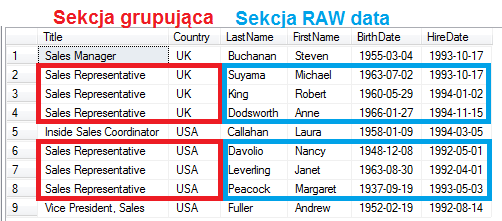
\includegraphics[scale=1]{sql/before-group-by.png}
    \end{center}
    \begin{minted}{sql}
        select Title, Country, COUNT(*) as EmQty
        from dbo.Employees
        GROUP BY Country,Title
    \end{minted}
    \begin{center}
        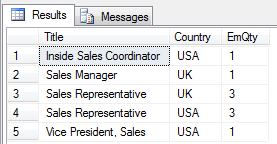
\includegraphics[scale=1]{sql/after-group-by.png}
    \end{center}

    \subsection{Podzapytania}

    Podzapytanie polega na umieszczeniu instrukcji SELECT wewnątrz innej instrukcji SELECT. Serwer bazodanowy w pierwszej kolejności wykona zapytania wewnętrzne. Wynik zapytania wewnętrznego zwracany jest do zapytania zewnętrznego.

    Podział podzapytań ze względu na korelację z zapytaniem nadrzędnym:
    \begin{itemize}
        \item podzapytania niepowiązane (nieskorelowane)
        \item podzapytania powiązane (skorelowane)
    \end{itemize}

    \subsubsection{Podzapytania niepowiązane}
    W podzapytaniach niepowiązanych wewnętrzne zapytanie jest wykonywane tylko raz. Zwraca jeden wynik. Zapytanie wewnętrzne jest niezależne od zewnętrznego i może być wykonane samodzielnie.

    Za pomocą poniższego zapytania możemy odczytać nazwę podkategorii, do której należy produkt posiadający ID o numerze 748.
    \begin{minted}{sql}
        SELECT b.Name
        FROM Production.ProductSubcategory b
        WHERE b.ProductSubcategoryID =
        (SELECT a.ProductSubcategoryID
        FROM Production.Product a
        WHERE a.ProductID = 748);
    \end{minted}

    Z tabeli Production.ProductSubcategory odczytujemy nazwy wszystkich podkategorii (kolumna Name).

    Następnie sprawdzamy warunek w zewnętrznej klauzuli WHERE.

    W celu sprawdzenia warunku należy wykonać wewnętrzne zapytanie. W zapytaniu wewnętrznym możemy wybrać tylko jedną wartość (wartość skalarna).

    \subsubsection{Podzapytania powiązane}

    Podzapytania powiązane (skorelowane) są bezpośrednio powiązane z zapytaniem nadrzędnym. Łącznikiem jest jeden lub więcej atrybutów, przekazywanych z zapytania nadrzędnego. Zapytanie wewnętrzne wykonywane jest osobno dla każdego wiersza zwróconego przez zapytanie zewnętrzne. Zwraca ono tyle wyników, ile jest rekordów w wyniku zapytania zewnętrznego.

    Ze względu na powiązanie z zapytaniem nadrzędnym, zapytanie wewnętrzne nie może być wykonane samodzielnie.
    \begin{minted}{sql}
        SELECT b.BusinessEntityID,
        (SELECT COUNT(a.AddressTypeID)
        FROM Person.BusinessEntityAddress as a
        WHERE a.BusinessEntityID = b.BusinessEntityID) as licz_zam
        FROM Person.Person as b
        ORDER BY licz_zam DESC;
    \end{minted}

    W powyższym przykładzie w zapytaniu wewnętrznym zliczana jest liczba rekordów w tabeli Person.BusinessEntityAddress. Zapytanie wewnętrzne uruchomione jest dla każdego rekordu z tabeli Person.Person, w przypadku którego BusinessEntityID jest takie samo jak BusinessEntityID w tabeli Person.BusinessEntityAddress.

    \newpage

    \section{Szeregowalność harmonogramów w bazach danych.}

    \begin{definition}
        \textbf{Harmonogram} - inaczej historia S zbioru n transakcji $T_1, \dots, T_n$ jest takim ciągiem wszystkich
        operacji transakcji, że dla każdej transakcji $T_i \in S$ operacje tej transakcji w S muszą występować w takiej samej
        kolejności, w jakiej występują w $T_i$. Operacje z różnych transakcji mogą się przeplatać.\\

        Rodzaje harmonogramów:
        \begin{itemize}
            \item \textbf{Harmonogram szeregowy} - operacje każdej transakcji są wykonywane kolejno, \textbf{bez przeplatania}
            operacji z różnych transakcji. Są nieefektywne.
            \item \textbf{Harmonogram szeregowalny} - jego wpływ na stan bazy danych jest taki sam jak pewnego
            harmonogramu szeregowego.
            \item \textbf{Harmonogram nieszeregowy} - harmonogram, który nie jest sekwencyjny.
        \end{itemize}
    \end{definition}

    \begin{definition}
        \textbf{Konflikt operacji}. Dwie operacje są w stanie konfliktu, jeśli spełnione są warunki:
        \begin{itemize}
            \item Należą do \textbf{różnych transakcji},
            \item Uzyskują dostęp do \textbf{tego samego elementu},
            \item \textbf{Przynajmniej jedna} z operacji jest \textbf{operacją zapisu} elementu.
        \end{itemize}
    \end{definition}

    \begin{definition}
        \textbf{Harmonogram pełny} - harmonogram zawierający wszystkie operacje z transakcji składowych, gdzie dla
        dowolnych dwóch \textbf{operacji}, które są w \textbf{konflikcie}, jedna z nich musi \textbf{poprzedzać} drugą
        w harmonogramie.
    \end{definition}

    \begin{definition}
        \textbf{Równoważność konfliktowa}. Mówimy, że dwa harmonogramy są równoważne konfliktowo, jeżeli
        \textbf{kolejność} wszystkich \textbf{operacji konfliktowych} jest w nich \textbf{taka sama}. Wyniki
        harmonogramów równoważnych konfliktowo są takie same.
    \end{definition}

    \begin{definition}
        \textbf{Szeregowalność konfliktowa}. Harmonogram S jest szeregowalny konfliktowo, jeżeli jest on
        \textbf{konfliktowo równoważny} pewnemu harmonogramowi \textbf{szeregowemu} S’. Możemy zmieniać kolejność
        niekonfliktowych operacji w S.\\

        Szeregowalność konfliktowa stanowi warunek wystarczający zachowania spójności danych.
    \end{definition}

    \begin{definition}
        \textbf{Równoważność perspektywiczna harmonogramów}. Harmonogram S i S' zawierają te same instrukcje i dla każdego
        elementu danych Q:
        \begin{itemize}
            \item Jeśli w S $T_k$ jest transakcją, która w
            harmonogramie czyta Q jako pierwsza, to w S' $T_k$ musi być transakcją, która czyta Q jako pierwsza.
            \item Jeśli w S $T_i$ czyta Q zapisany przez $T_j$, to w S' $T_i$ czyta Q zapisany przez $T_j$.
            \item Jeśli w S  $T_m$ jest ostatnią transakcją, która
            zapisuje Q, to w S' $T_m$ jest ostatnią transakcją, która zapisuje Q.
        \end{itemize}
    \end{definition}

    \begin{definition}
        \textbf{Szeregowalność perpektywiczna}. Harmonogram szeregowalny perspektywicznie jest harmonogramem
        \textbf{równoważnym perspektywicznie} jakiemuś harmonogramowi szeregowemu.

        Szeregowalność perspektywiczna to \textbf{szeregowalność konfliktowa z dodatkowymi ograniczeniami} operacji zapisów:
        \begin{itemize}
            \item każda operacja w(x) jest poprzedzona r(x),
            \item wartość zapisana przez operację w(x) \textbf{jest nie-stałą funkcją} zależną tylko od wartości r(x).
        \end{itemize}
    \end{definition}

    \newpage

    \section{Definicja cyfrowego układu kombinacyjnego - przykłady układów kombinacyjnych i ich implementacje.}

    \begin{definition}
        \textbf{Układ kombinacyjny} to taki układ logiczny, w którym każda kombinacja wartosci zmiennych wejściowych
        jednoznacznie określa kombinację wartości zmiennych wyjściowych.\\

        Układy kombinacyjne opisujemy za pomocą bramek logicznych. Można też za pomocą tablicy prawdy.
    \end{definition}

    \begin{definition}
        \textbf{Bramka logiczna} to układ elektroniczny realizujący funkcję logiczną jednej lub wielu zmiennych
        (w podstawowej wersji dwóch).
    \end{definition}

    \begin{figure}[H]
        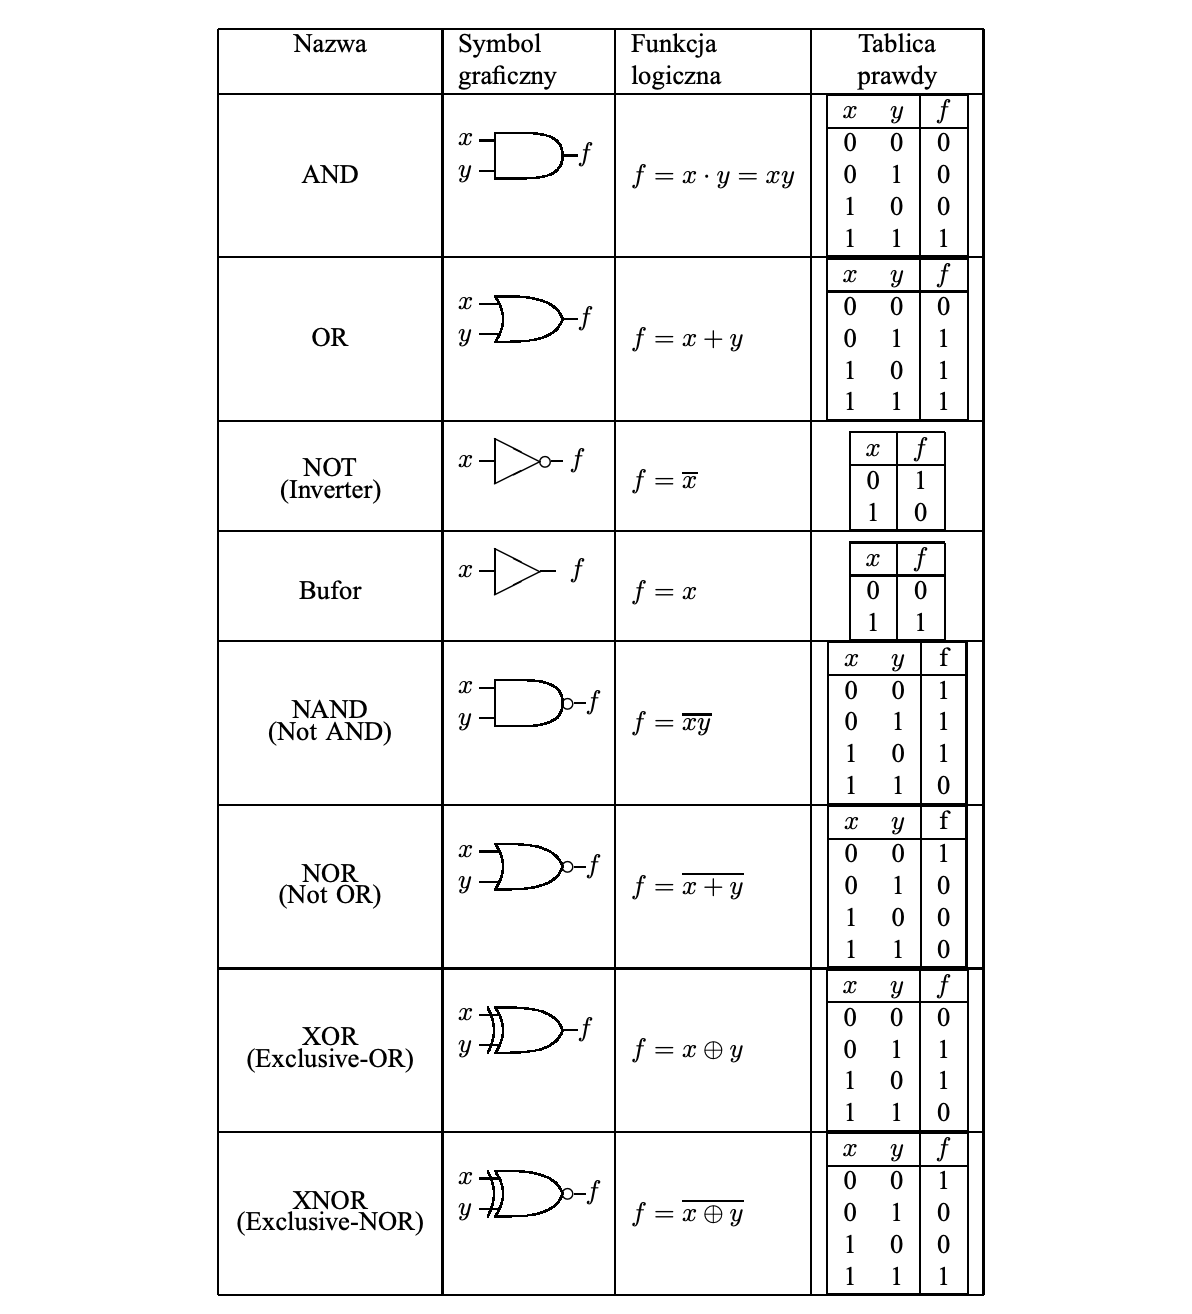
\includegraphics[width=\linewidth]{uk/bramki.png}
    \end{figure}

    \subsection{Układy arytmetyczne.}

    \subsubsection{Półsumator (Half Adder).}
    Zmiennymi wejściowymi półsumatora są bity składników sumy \textit{(x, y)}. Zmiennymi wyjsciowymi są bity
    sumy \textit{s} i przeniesienia \textit{c}.

    \begin{figure}[H]
        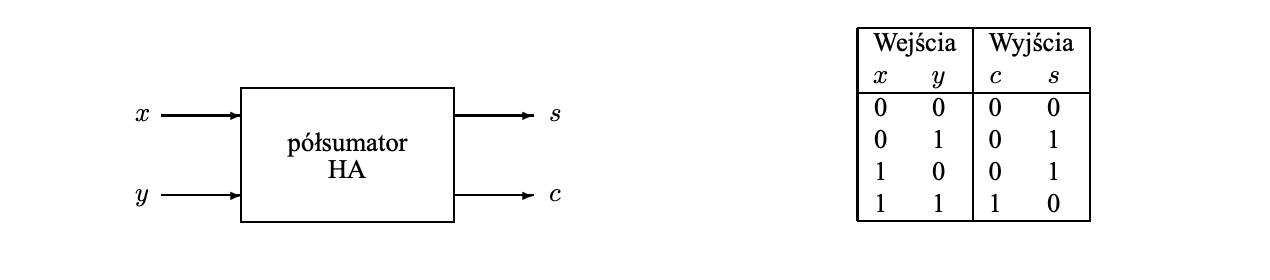
\includegraphics[width=\linewidth]{uk/ha.png}
    \end{figure}

    Z tablicy prawdy półsumatora otrzymujemy następujące funkcje logiczne:
    \begin{gather*}
        s(x,y) = \sum (1,2) = \bar{x}y + x\bar{y} = x \oplus y\\
        c(x,y) = \sum (3) = xy\\
    \end{gather*}

    na podstawie których możemy zbudować schemat logiczny półsumatora:

    \begin{figure}[H]
        
\includegraphics[width=\linewidth]{uk/ha_l.png}
    \end{figure}

    \subsubsection{Sumator (Full Adder).}
    Układ kombinacyjny dodający trzy cyfry dwójkowe. Ma trzy wejścia. Dwie ze zmiennych wejściowych \textit{(x, y)}
    reprezentują bity składników sumy. Trzecie wejście \textit{(z)} reprezentuje przeniesienie z poprzedniej, mniej
    znaczącej pozycji. Zmiennymi wyjściowymi są bity sumy \textit{s} i przeniesienia \textit{c}.

    \begin{figure}[H]
        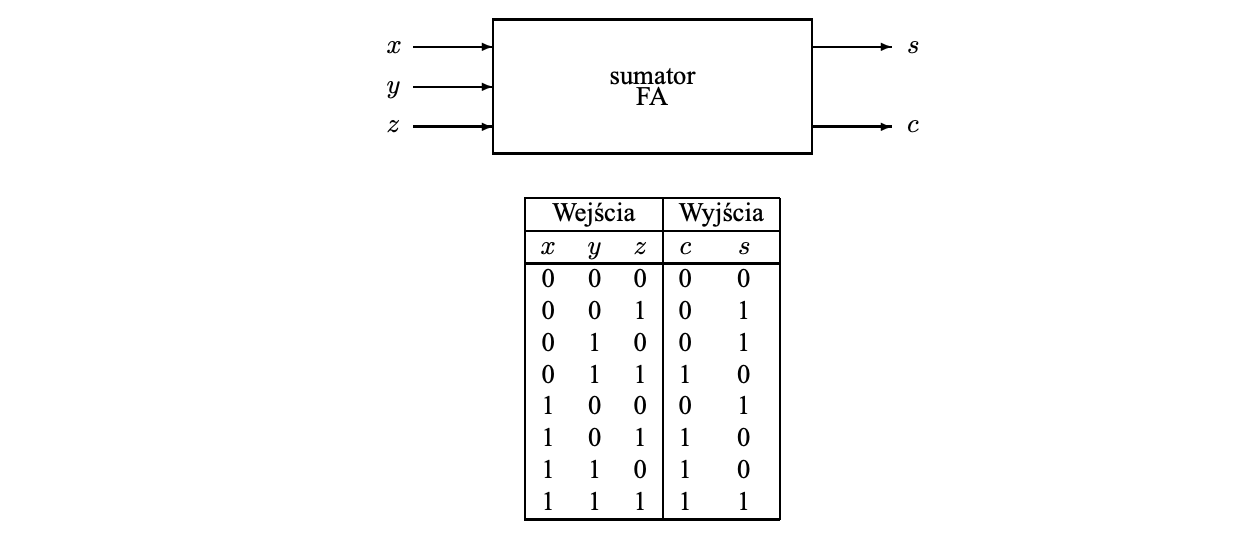
\includegraphics[width=\linewidth]{uk/fa.png}
    \end{figure}

    \begin{gather*}
        s(x,y) = \sum (1,2,4,7) = \bar{x}\bar{y}z + \bar{x}y\bar{z} + xyz\\
        c(x,y) = \sum (3,5,6,7) = xz + yz + xy\\
    \end{gather*}

    \begin{figure}[H]
        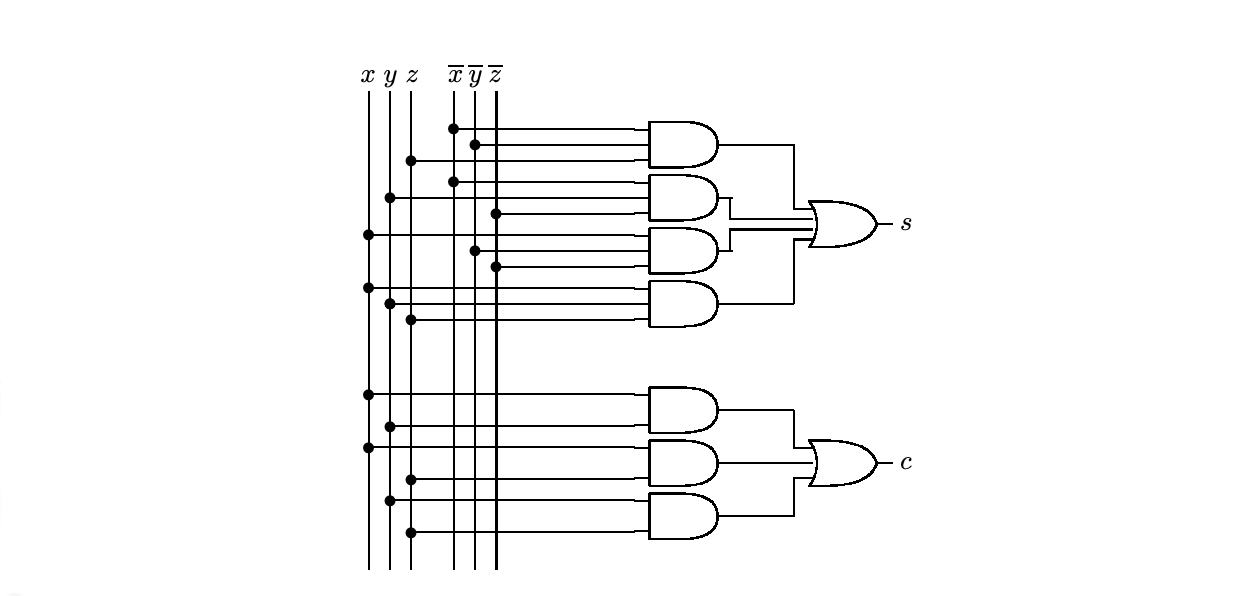
\includegraphics[width=\linewidth]{uk/fa_l.png}
    \end{figure}

    Schemat blokowy 4-bitowego sumatora równoległego (sumatora dwóch liczb czterobitowych a i b):

    \begin{figure}[H]
        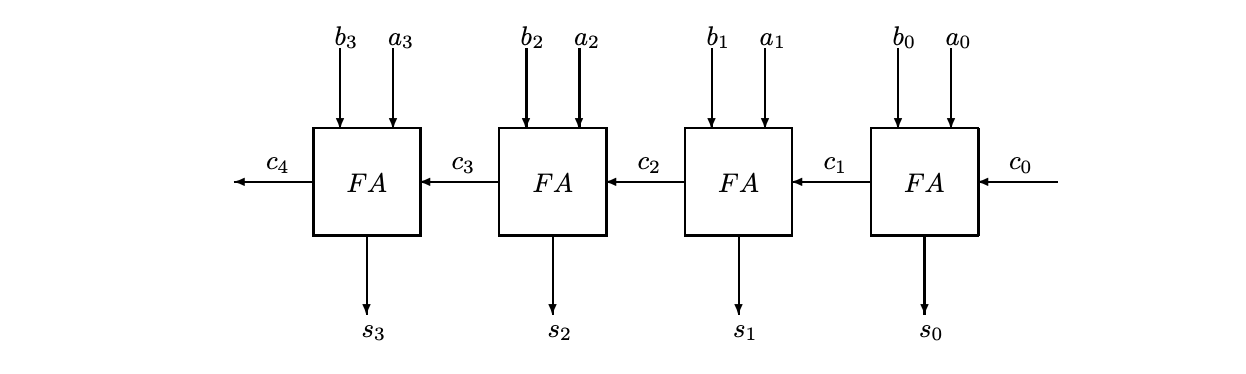
\includegraphics[width=\linewidth]{uk/fa_4.png}
    \end{figure}

    \subsubsection{Dekoder.}
    Układ kombinacyjny mający $n$ wejść i $m \leq 2^n$ wyjść, w którym każdej kombinacji zmiennych wejściowych
    odpowiada pojawienie się jedynki logicznej tylko na jednym wyjściu, na pozostałych wyjściach zera.

    \begin{figure}[H]
        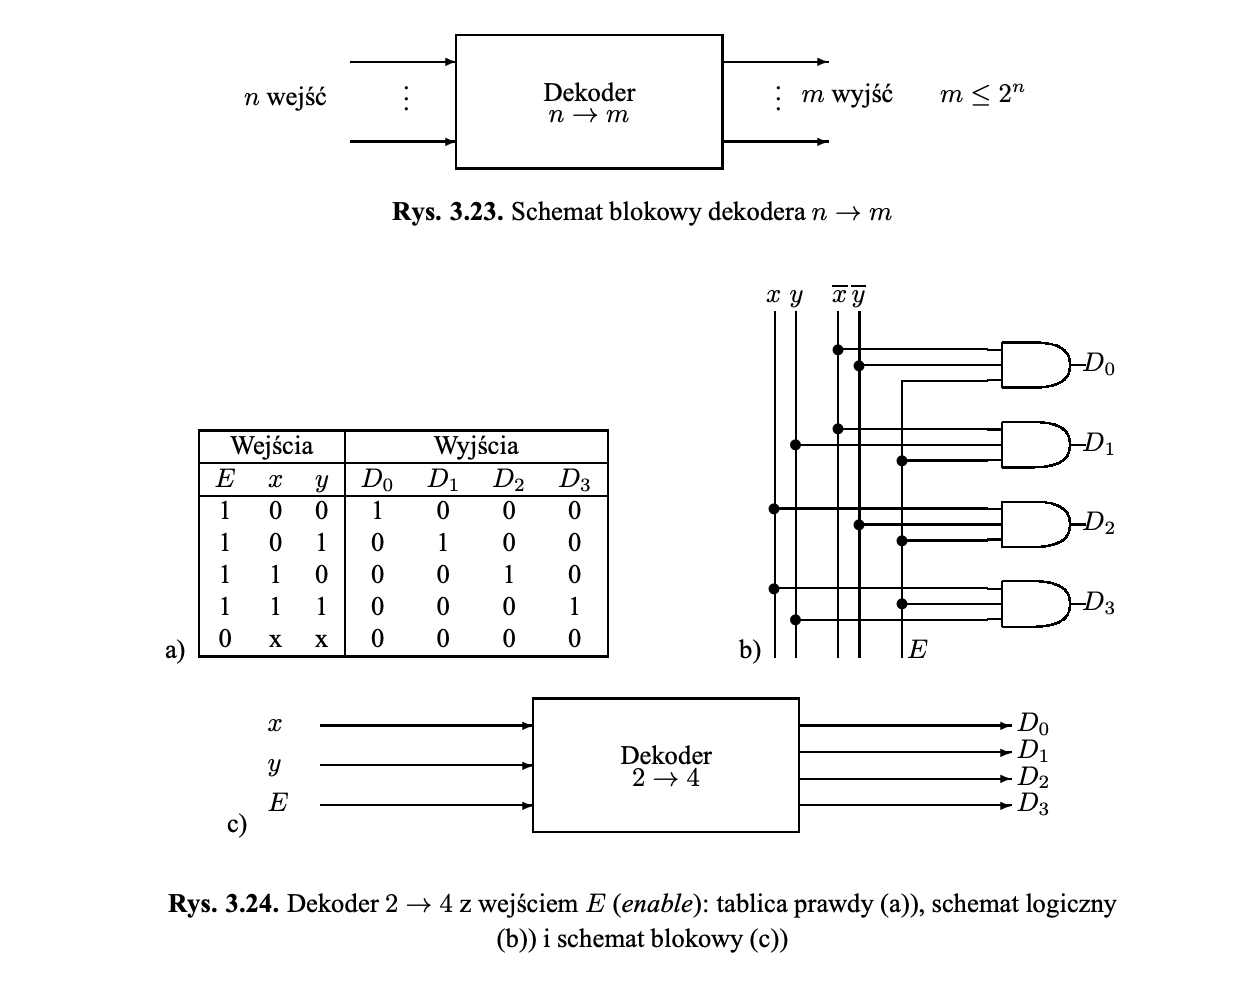
\includegraphics[width=\linewidth]{uk/dek.png}
    \end{figure}

    \textbf{Koder to układ kombinacyjny działający odwrotnie do dekodera}.

    \subsubsection{Multiplekser.}
    Układ kombinacyjny wybierający informację dwójkową na jednej z linii wejściowych i kierujący ją na jedną linię
    wyjściową. Wybór linii wejściowej jest określany przez linie sterujące.

    \begin{figure}[H]
        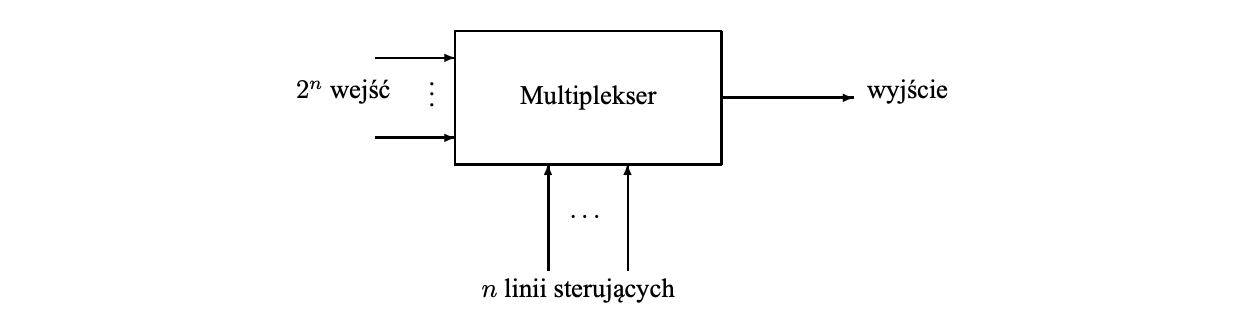
\includegraphics[width=\linewidth]{uk/mul.png}
    \end{figure}

    Linie wejściowe $(d_0, d_1, d_2, d_3)$ są doprowadzone do bramek AND, których wyjścia sa doprowadzone do bramki
    OR. W danej chwili tylko jedna linia wejściowa jest połączona z wyjściem \textit{y}. O wyborze wjeścia połączonego
    decydują linie sterujące $s_0, s_1$.

    \begin{figure}[H]
        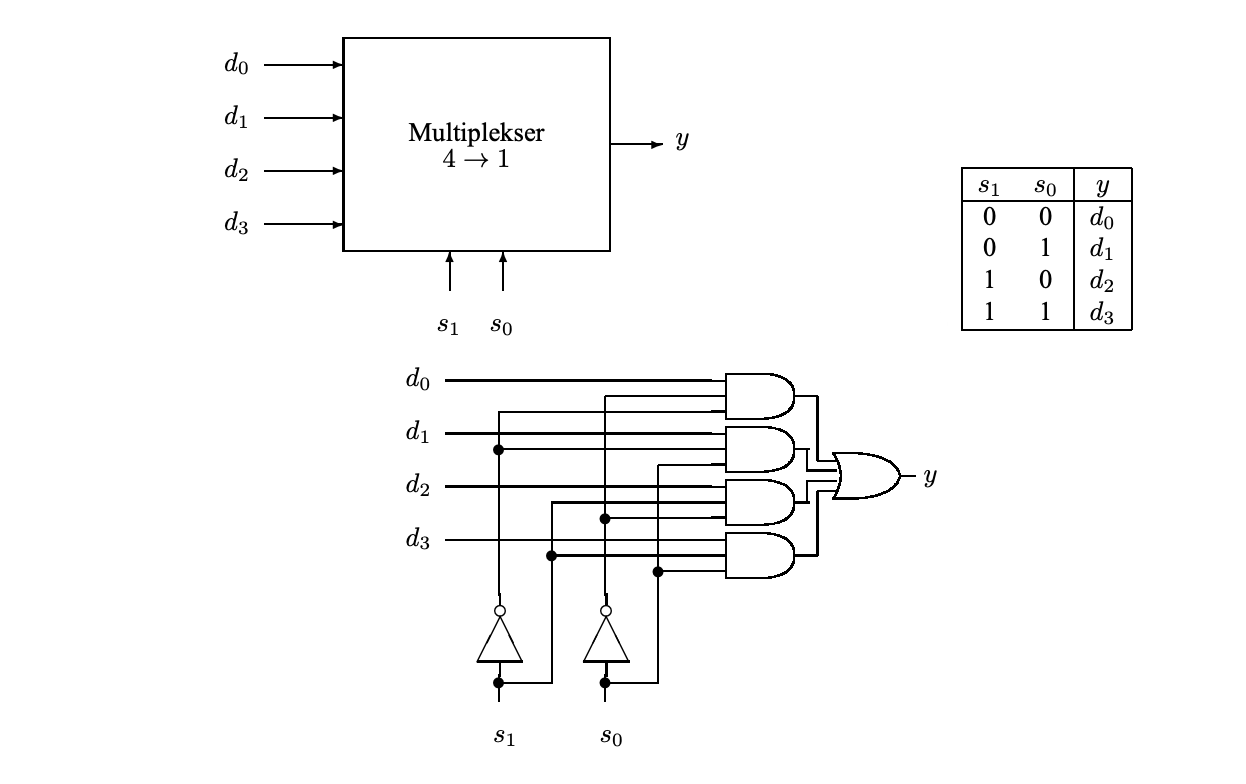
\includegraphics[width=\linewidth]{uk/mul_l.png}
    \end{figure}

    \newpage

    \section{Definicja cyfrowego układu sekwencyjnego - przykłady układów sekwencyjnych i ich implementacje.}

    \begin{definition}
        Układem sekwencyjnym (ang. sequential logic circuits) nazywamy układ, w którym poziomy sygnałów wyjściowych zależą nie tylko od aktualnego stanu poziomów sygnałów na jego wejściu,
        ale również od stanu poziomów, które występowały uprzednio. Oznacza to, że układy te zawierają elementy pamiętające i nazywane są czasem układami kombinacyjnymi z pamięcią.
    \end{definition}

    \begin{definition}
        \textbf{Przerzutnik RS} (Reset-Set) - jest najprostszym rodzajem przerzutnika zbudowanego z 2 bramek NOR (w innej wersji NAND). Posiada dwa wejścia: S i R; oraz dwa wyjścia Q i $\bar{Q}$.
        Zasadę jego działania przedstawia poniższa tabelka:
        \begin{table}[H]
            \center
            \begin{tabular}{|c|c|c|c|}
                \hline
                \textbf{R} & \textbf{S} & $\mathbf{Q_{n-1}}$ & $\mathbf{Q_n}$ \\ \hline
                0 & 0 & 0 & 0              \\ \hline
                0 & 0 & 1 & 1              \\ \hline
                0 & 1 & X & 1              \\ \hline
                1 & 0 & X & 0              \\ \hline
                1 & 1 & X & N              \\ \hline
            \end{tabular}
        \end{table}
        Jak widać, po podaniu 1 na wejście S, wyjście Q niezależnie od swojego poprzedniego stanu jest ustawiane na 1, natomiast podanie 1 na wejście R, powoduje ustawienie wyjścia Q na stan 0 niezależnie od jego poprzedniego stanu. Gdy ani na wejście S, ani na wejście R nie podamy 1, wtedy przerzutnik ``pamięta'' poprzedni stan (stan wyjścia Q się nie zmienia), natomiast podanie na oba wejścia 1 jest niedozwolone, ponieważ powoduje ustawienie stanu 0 na obu wyjściach, co jest niezgodne z założeniami (wyjście $\bar{Q}$ ma być zawsze negacją wyjścia Q). \\
        \noindent Przykładowy schemat blokowy przerzutnika (na bramkach NOR): \\

        \begin{center}
            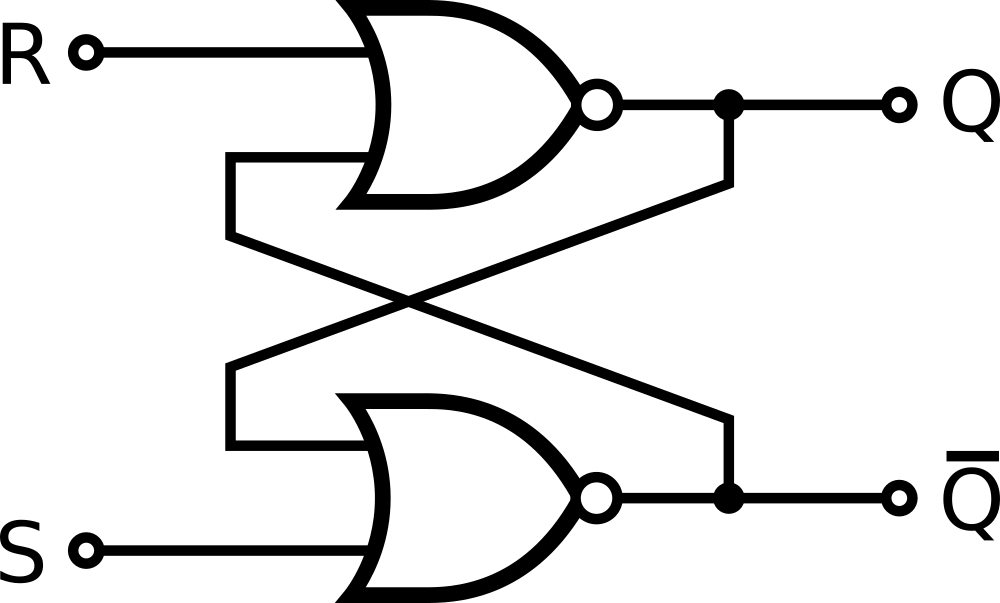
\includegraphics[width=0.5\linewidth]{sequentials/rs.png}
        \end{center}

    \end{definition}




    \begin{definition}
        \textbf{Przerzutnik D} (Delay) - jest pewną modyfikacją przerzutnika RS. Ma on wejście D oraz C (Clock). Jego działanie polega na przekazaniu stanu wejścia D na wyjście Q w momencie ``tyknięcia'' zegara
        (podania stanu 1) na wejściu C.
        Zasadę jego działania przedstawia poniższa tabelka:
        \begin{table}[H]
            \center
            \begin{tabular}{|c|c|c|c|}
                \hline
                \textbf{D} & $\mathbf{Q_{n-1}}$ & $\mathbf{Q_n}$ \\ \hline
                0 & 0 & 0              \\ \hline
                0 & 1 & 0              \\ \hline
                1 & 0 & 1              \\ \hline
                1 & 1 & 1              \\ \hline
            \end{tabular}
        \end{table}

        lub równoważnie:

        \begin{table}[H]
            \center
            \begin{tabular}{|c|c|c|c|}
                \hline
                \textbf{D} & $\mathbf{Q_{n-1}}$ & $\mathbf{Q_n}$ \\ \hline
                0 & X & 0              \\ \hline
                1 & X & 1              \\ \hline
            \end{tabular}
        \end{table}

        Jak widać w przeciwieństwie do samego przerzutnika RS, który jest asynchroniczny, tutaj mamy wejście zegarowe, które synchronizuje jego pracę. \\
        \noindent Przykładowy schemat blokowy przerzutnika (w tym przypadku część odpowiedzialna za przerzutnik RS została zbudowana na bramkach NAND - ta wersja nazywa się SR,
        ponieważ w przypadku podania na oba wejścia 1, na obu wyjściach pojawi się stan 1 - Set ma priorytet): \\

        \begin{center}
            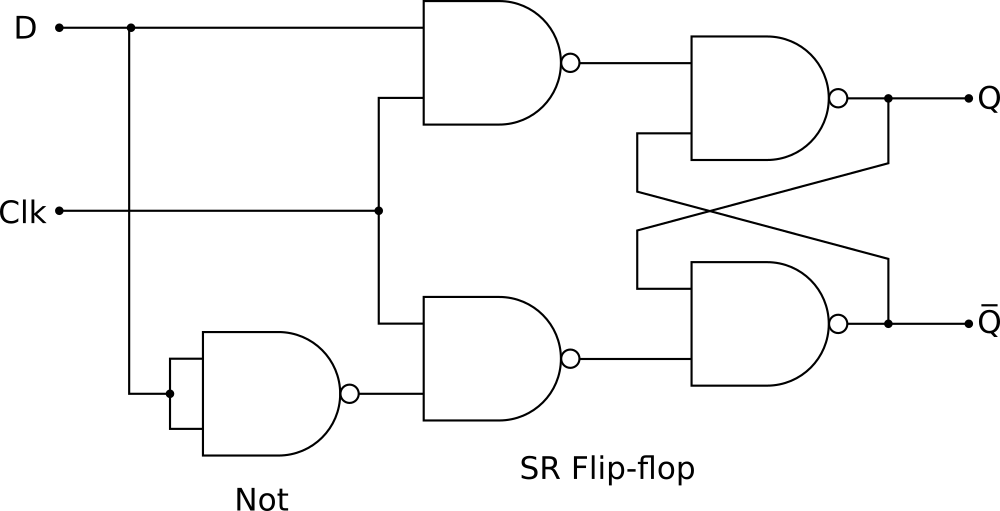
\includegraphics[width=0.5\linewidth]{sequentials/d.png}
        \end{center}

    \end{definition}



    \begin{definition}
        \textbf{Przerzutnik JK} - podobnie jak przerzutnik D jest synchroniczny oraz powstał poprzez modyfikację przerzutnika RS (SR). W tej wersji pozbyto się kłopotliwego stanu, gdy na oba wejścia przerzutnika RS podana zostanie 1.
        Przerzutnik JK posiada 3 wejścia: J, K oraz Clock. Porównując RS do JK: odpowiednikiem wejścia S jest wejście J, a odpowiednikiem wejścia R jest wejście K.
        Zasadę działania przerzutnika JK przedstawia poniższa tabelka:
        \begin{table}[H]
            \center
            \begin{tabular}{|c|c|c|c|}
                \hline
                \textbf{J} & \textbf{K} & $\mathbf{Q_{n-1}}$ & $\mathbf{Q_n}$ \\ \hline
                0 & 0 & 0 & 0              \\ \hline
                0 & 0 & 1 & 1              \\ \hline
                1 & 0 & X & 1              \\ \hline
                0 & 1 & X & 0              \\ \hline
                1 & 1 & 0 & 1              \\ \hline
                1 & 1 & 1 & 0              \\ \hline
            \end{tabular}
        \end{table}
        Jak widać w przypadku podania na oba wejścia (J i K) 1, przerzutnik zmienia stan wyjścia na odwrotny w stosunku do tego, który był przed podaniem sygnału zegarowego. \\
        \noindent Przykładowy schemat blokowy przerzutnika (na bramkach NAND): \\

        \begin{center}
            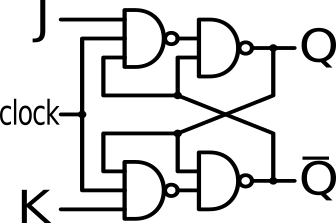
\includegraphics[width=0.5\linewidth]{sequentials/jk.png}
        \end{center}

    \end{definition}

    \newpage

    \section{Minimalizacja funkcji logicznych.}

    \subsection{Minimalizacja z wykorzystaniem algebry Boole'a}
    \begin{definition}
        Minimalizacja z wykorzystaniem algebry Boole'a polega na zapisaniu funkcji w postaci sumy stanów wejść, dla których funkcja przyjmuje wratość 1, a następnie wykorzystując prawa algebry Boole'a uproszczenie jej.
    \end{definition}

    \subsection{Minimalizacja z wykorzystaniem tablic Karnaugha}
    \begin{definition}
        \textbf{Tablica Karnaugha} składa się z pól reprezentujących wszystkie kombinacje zmiennych naszej funkcji, którą chcemy zminimalizować jednak są one ułożone w specyficzny sposób:
        każde sąsiednie dwa pola (pól po ukosie nie uznajemy za sąsiednie) muszą się różnić wartością tylko jednej zmiennej.
        Za sąsiednie pola uważamy również pola na krańcach danego wiersza i danej kolumny - możemy więc traktować tą tablicę jako tablicę cykliczną. \\

        Przykłady gotowych tablic Karnauhga: \\

        \begin{center}
            Dla dwóch zmiennych \\
            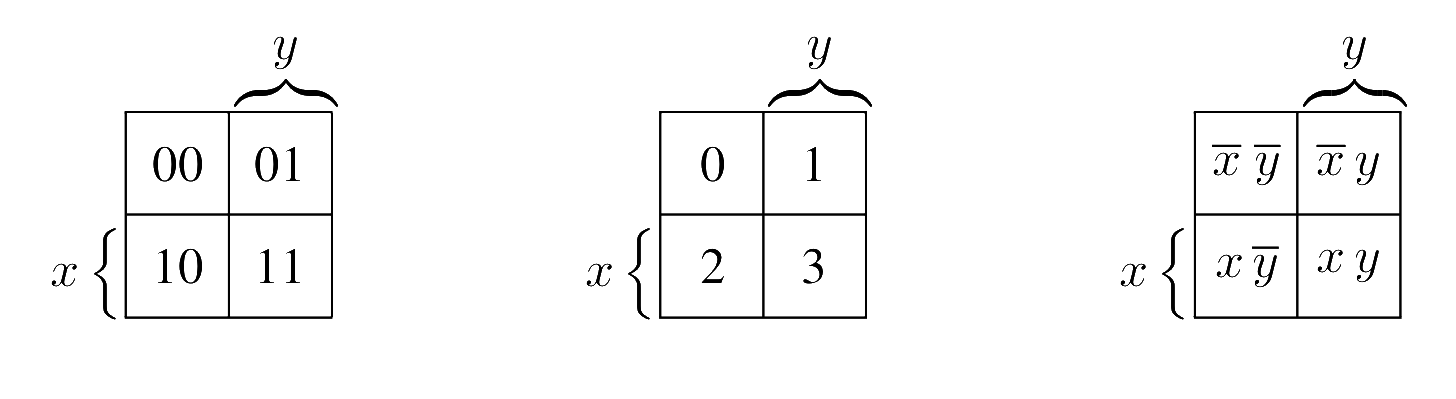
\includegraphics[width=\linewidth]{karnaugh/2-vars.png}

            Dla trzech zmiennych \\
            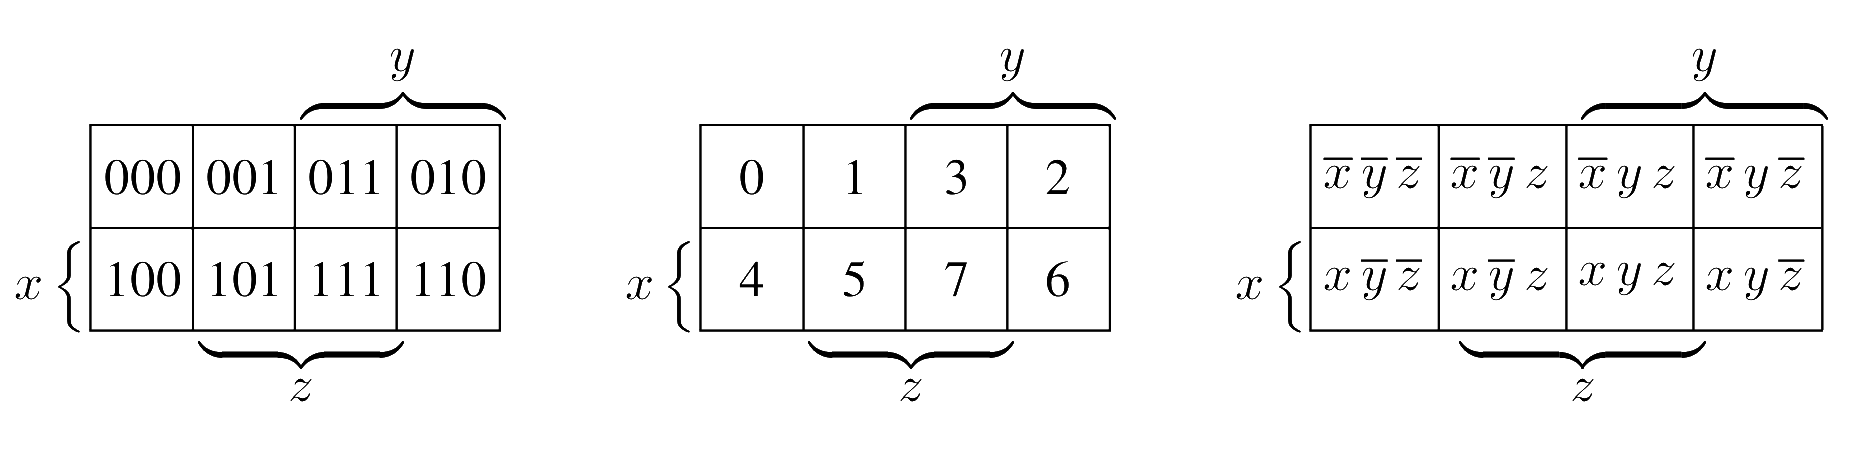
\includegraphics[width=\linewidth]{karnaugh/3-vars.png}

            Dla czterech zmiennych \\
            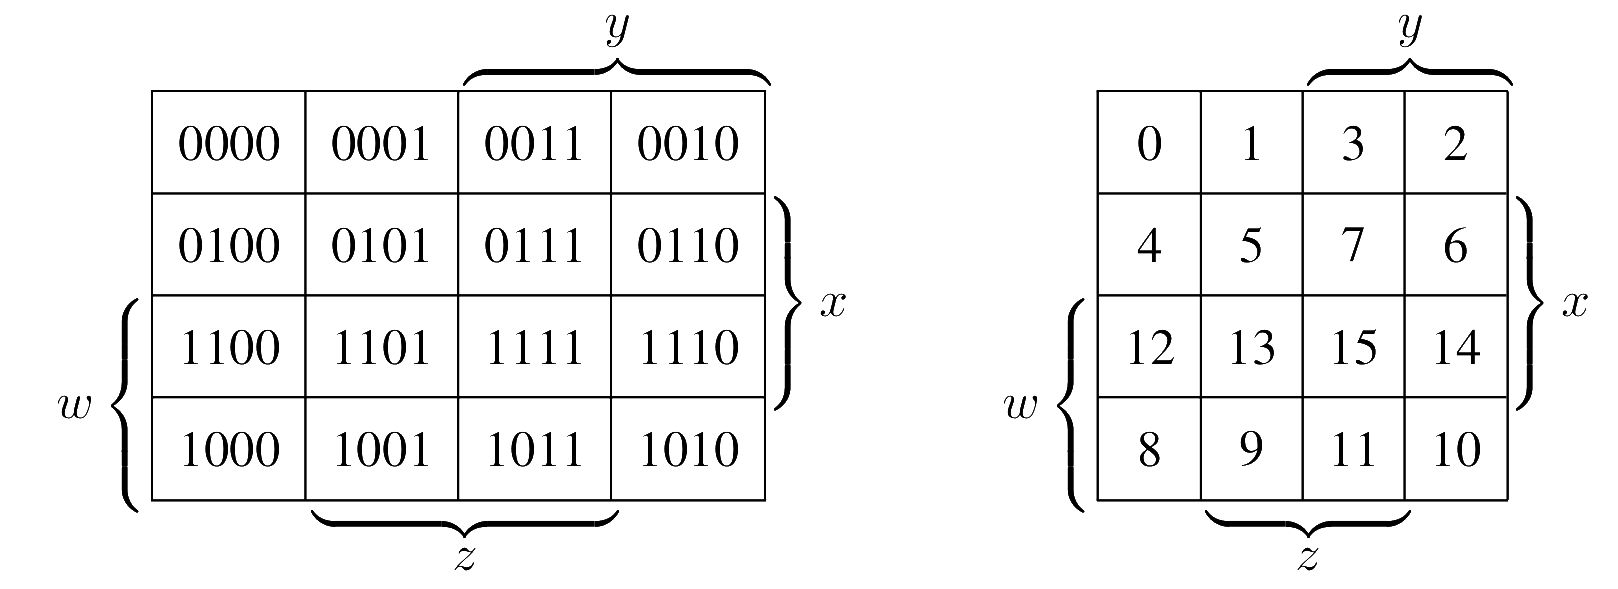
\includegraphics[width=\linewidth]{karnaugh/4-vars.png}
        \end{center}

        Przy pomocy tablic Karnaugha możemy minimalizować funkcję o maksymalnie 6 zmiennych.
    \end{definition}


    \newpage

    \section{Programowalne układy logiczne PLD (ROM, PAL, PLA).}

    Programowalne układy logiczne (Programmable Logic Devices / PLD) dzielą się na:
    \begin{itemize}
        \item Read Only Memory (ROM)
        \item Programmable Array Logic (PAL)
        \item Programmable Logic Array (PLA)
    \end{itemize}

    \subsection{ROM}
    Wejście jest '\textit{hard-wired}` i zawiera wszystkie możliwe mintermy, wyjście jest programowalne.
    \begin{center}
        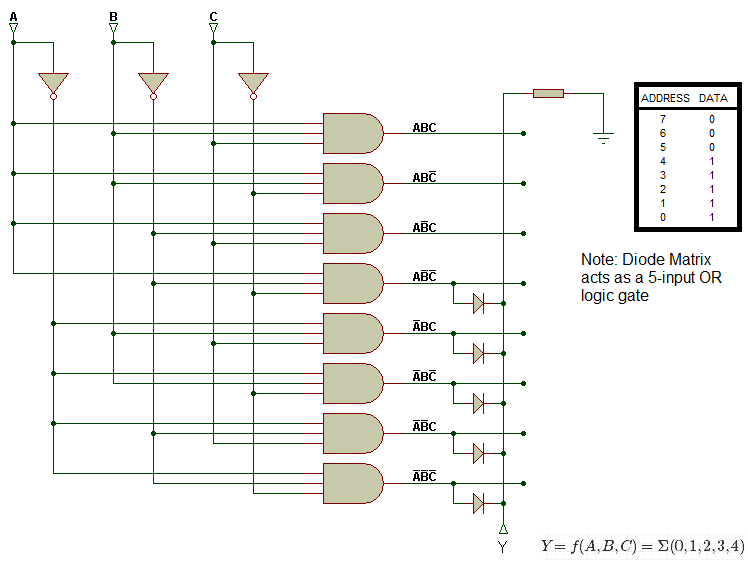
\includegraphics[scale=0.7]{rom.png}
    \end{center}

    \subsection{PAL}
    Układy PAL zawierają część nieprogramowalną (wbudowane bramki OR) oraz programowalną
    matrycę bramek AND.
    Wejście jest programowalne, wyjście jest '\textit{hard-wired}`.
    \begin{center}
        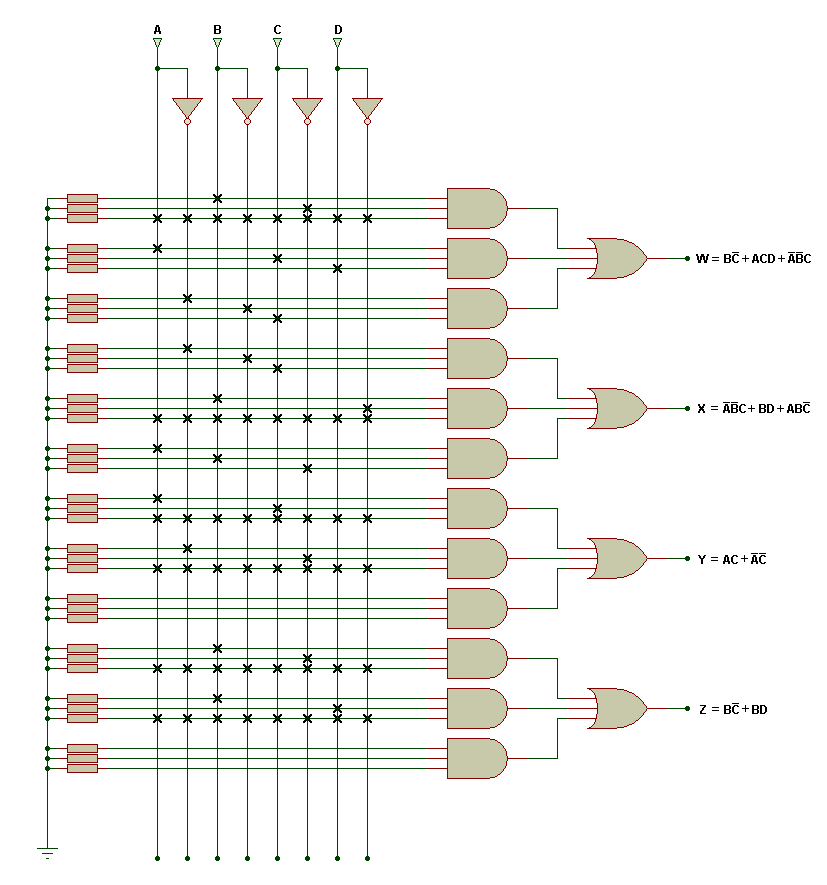
\includegraphics[scale=0.7]{pal.png}
    \end{center}

    \subsection{PLA}
    Układy PLA zawierają część programowalną matrycę bramek OR oraz programowalną
    matrycę bramek AND.
    Wejście jest programowalne, wyjście jest programowalne.
    \begin{center}
        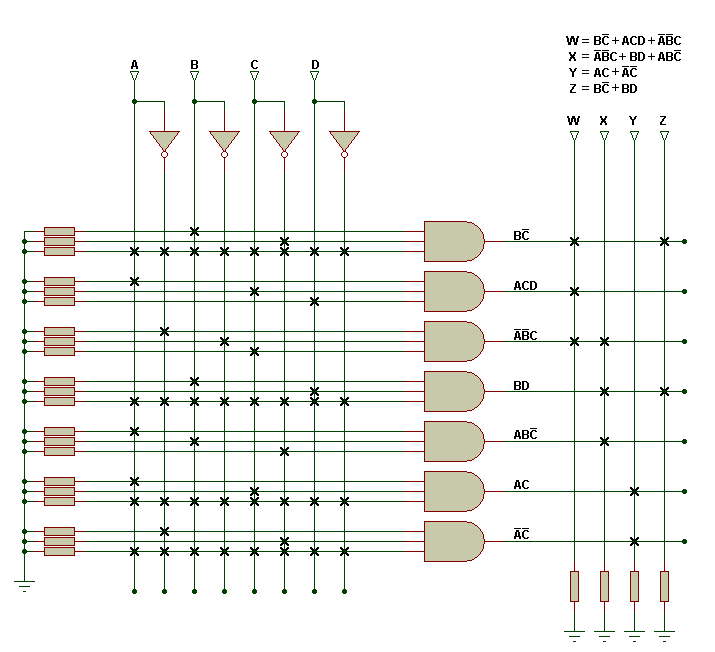
\includegraphics[scale=0.7]{pla.png}
    \end{center}

    \textbf{PLA} vs \textbf{PAL}:
    \begin{itemize}
        \item PLA konstruuje się bramkami AND i OR. PAL tak samo, ale liczba
        OR jest ustalona.
        \item PLA są droższe w produkcji
        \item PAL są szybsze
        \item Liczba funkcji zaimplementowanych w PAL jest ograniczona,
        układy PAL są mniej elastyczne i programowalne niż PLA
    \end{itemize}
    \newpage

    \section{Schemat blokowy komputera (maszyna von Neumanna).}

    \begin{center}
        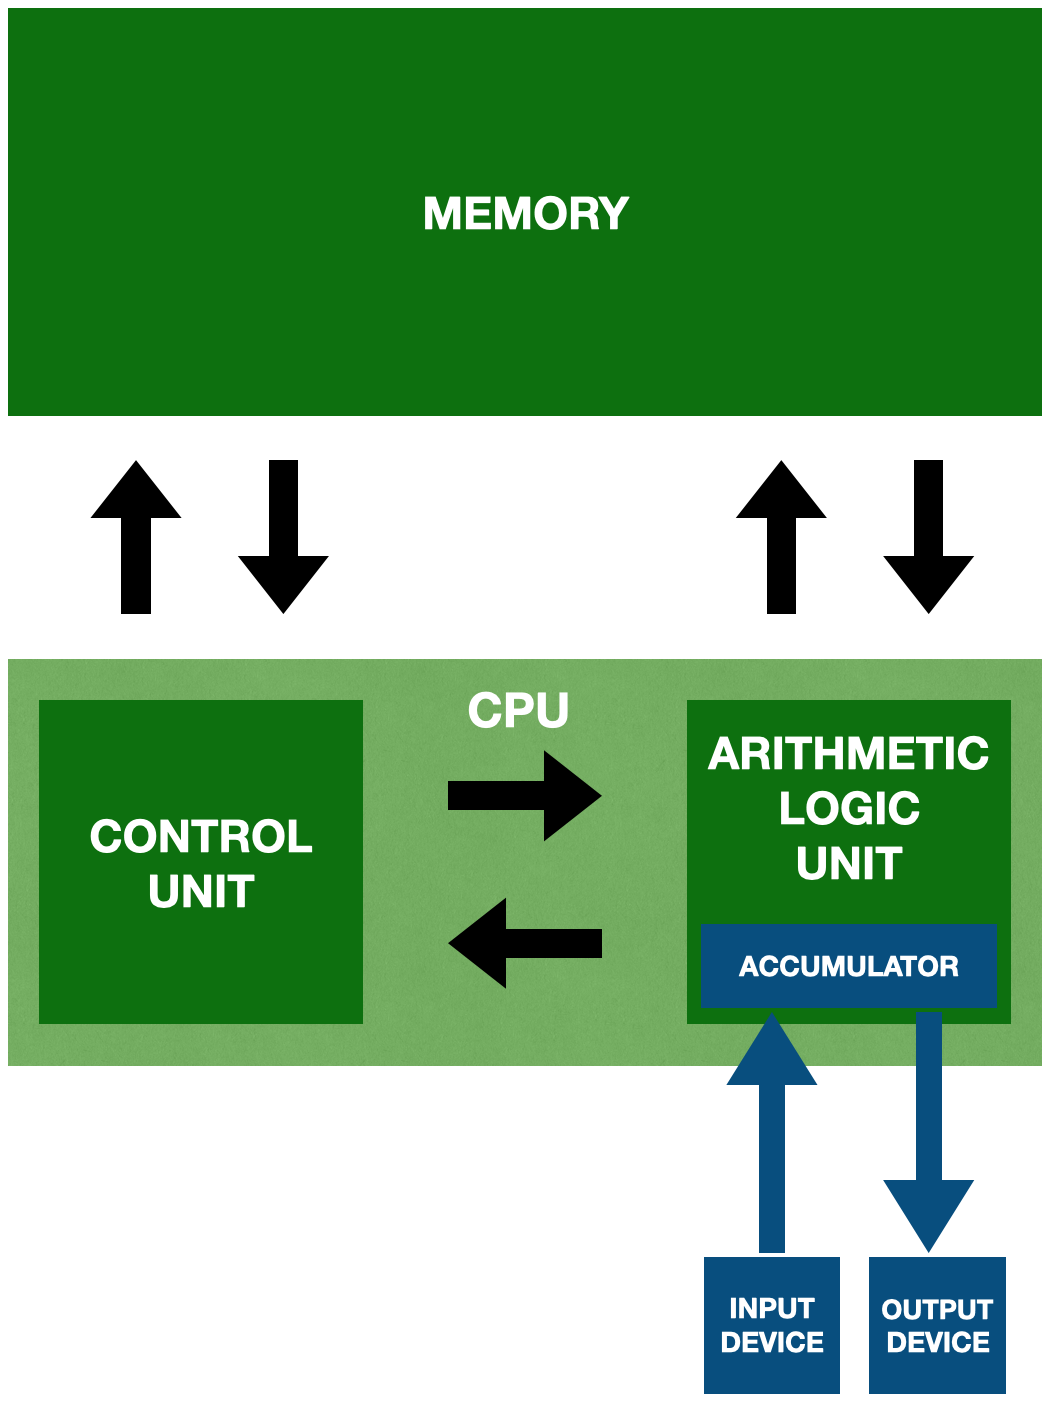
\includegraphics[width=0.62\textwidth]{von_neumann.png}
    \end{center}

    Architektura von Neumanna to rodzaj architektury cyfrowego komputera opracowana w 1945 przez Johna von Neumanna.
    Składa się z następujących części:

    \begin{itemize}
        \item Pamięci - zawiera zarówno dane, jak i instrukcji
        \item CPU, Central Processing Unit, Procesora. CPU składa się z:
        \begin{itemize}
            \item Jednostki kontrolnej (nadzorującej)
            \item Jednostki arytmetyczno-logicznej wykonującej podstawowe operacje przetwarzania informacji.
        \end{itemize}
    \end{itemize}

    I/O:
    \begin{itemize}
        \item Akumulator, wchodzący w skład jednostki arytmetyczno-logicznej
        \item Urządzenia wejścia
        \item Urządzenia wyjścia
    \end{itemize}

    Cechy architektury von Neumanna:
    \begin{itemize}
        \item Jednolitość pamięci
        \begin{itemize}
            \item Możliwość uruchomienia samomodyfikującego się programu
            \item Dzielenie pamięci instrukcji z pamięcią danych może prowadzić do bottlenecków (w tym celu wprowadza się cache)
        \end{itemize}
        \item Skończona liczba rozkazów
        \item Informacje są przetwarzane poprzez sekwencyjny odczyt kolejnych instrukcji z pamięci i ich wykonanie przez procesor
    \end{itemize}

    Warto zapamiętać:
    \begin{itemize}
        \item Niemalże wszystkie cyfrowe, elektroniczne współczesne komputery są oparte na architekturze von Neumanna
        \item Architektura von Neumanna pozwoliła na oddzielenie programu od procesora
        \item Istnieje architektura Harvardzka, oddzielająca pamięć z rozkazami od pamięci z danymi.
    \end{itemize}

    \newpage

    \section{Zarządzanie procesami: stany procesu, algorytmy szeregowania z wywłaszczaniem.}
    \subsection{Proces}
    Proces służy do \textbf{organizowania wykonywania programu} w ten sposób, że stanowi on powiązanie \textbf{niezbędnych zasobów systemu komputerowego} i umożliwia \textbf{kontrolę stanu} tych zasobów związaną z wykonywaniem programu.


    \subsection{Proces a program}
    Program
    \begin{itemize}
        \item Zbiór instrukcji
        \item Element procesu znajdujący się w segmencie kodu
        \item Stan nie ulega modyfikacji w czasie wykonywania
        \item Wykorzystuje dodatkowe zasoby (procesor, pamięć itp.)
    \end{itemize}

    Stan procesu ulega zmianie: zmienia się stan wykonywania programu podobnie jak stan większości zasobów z tym związanych. Zmianie w wyniku wykonywania procesu ulega np. segment danych, segment stosu, stan rejestrów procesora itp. Procesem jest więc cały ten kontekst niezbędny do wykonania programu. Wyodrębnienie procesu wiąże się z współbieżnością przetwarzania. W systemie może istnieć wiele procesów (wiele niezależnych przetwarzań), stąd ważne jest utrzymanie informacji o tym, które zasoby przedzielone na potrzeby każdego przetwarzania.

    \subsection{Zarządzanie procesami}

    Fragmenty kodu jądra związane z obsługą procesów i zasobów nazywa się zarządcami.
    Wyróżnia się:
    \begin{itemize}
        \item \textbf{zarządców procesów} (grupują i wykonuja funkcje obsługi procesów)
        \item \textbf{zarządców zasobów} (kontrolują stan zajętości zasobów i realizację żądań procesów)
    \end{itemize}

    \subsection{Stany procesu}

    W zależności od stanu wykonywania programu i dostępności zasobów można wyróżnić następujące, ogólne stany procesu:

    \begin{itemize}
        \item \textbf{Nowy} — formowanie procesu, czyli gromadzenie zasobów niezbędnych do rozpoczęcia wykonywania procesu, z wyjątkiem procesora (kwantu czasu procesora), a po zakończeniu formowania oczekiwanie na przyjęcie do kolejki procesów gotowych.
        \item \textbf{Wykonywany} — wykonywanie instrukcji programu danego procesu i wynikająca z ich wykonywania zmiana stanu odpowiednich zasobów systemu.
        \item \textbf{Oczekujący} — zatrzymanie wykonywania instrukcji programu danego procesu ze względy na potrzebę przydziału dodatkowych zasobów, konieczność otrzymania danych lub osiągnięcia odpowiedniego stanu przez otoczenie procesu (np. urządzenia zewnętrzne lub inne procesy).
        \item \textbf{Gotowy} — oczekiwanie na przydział kwantu czasu procesora (dostępność wszystkich niezbędnych zasobów z wyjątkiem procesora).
        \item \textbf{Zakończony} — zakończenie wykonywania programu, zwolnienie większości zasobów i oczekiwanie na możliwość przekazania informacji o zakończeniu innym procesom lub jądru systemu operacyjnego.
        Pozostawanie procesu z stanie zakończony (w systemach uniksopodobnych zwany zombi ) spowodowane jest przetrzymywaniem pewnych informacji o procesie po jego zakończeniu (np. statusu zakończenie). Całkowite usunięcie procesu mogłoby oznaczać zwolnienie pamięci i utratę tych informacji.
    \end{itemize}

    \subsection{Cykl zmiany stanów procesu}

    \begin{itemize}
        \item Gotowy $\rightarrow$ Wykonywany \\
        Decyzja modułu szeregującego procesy (planista przydziału procesora), która oparta jest na priorytetach procesów. Jeżeli w systemie jest jedna jednostka przetwarzająca (procesor), to w stanie wykonywany może być tylko jeden proces, podczas gdy pozostałe procesy znajdują się w innych stanach (w szczególności w stanie gotowy).
        \item Wykonywany $\rightarrow$ Gotowy \\
        Oznacza wywłaszczenie procesu z procesora. Wywłaszczenie może być następstwem:
        \begin{enumerate}
            \item Upływu kwantu czasu. \\
            W systemach z \textbf{podziałem czasu} proces otrzymuje tylko kwant czasu na wykonanie kolejnych instrukcji.
            Upływ kwantu czasu odmierzany jest przez przerwanie zegarowe, a po stwierdzeniu wyczerpania kwantu czasu następuje przełączenie kontekstu i kolejny kwant czasu otrzymuje inny proces (rotacyjny algorytm planowania przydziału procesora).
            \item Pojawienia się procesu gotowego z wyższym priorytetem.\\
            W systemie z \textbf{dynamicznymi priorytetami} przerwanie zegarowe lub inne zdarzenie obsługiwane przez jądro wyznacza momenty czasu, w którym przeliczane są priorytety procesów. Jeśli stosowane jest wywłaszczeniowe podejście do planowania przydziału procesora, oparte na priorytecie, proces o najwyższym priorytecie otrzymuje procesor. Więcej szczegółów zostanie omówionych w następnym module.
        \end{enumerate}
    \end{itemize}

    \subsection{Szeregowanie procesów}

    Szeregowanie (planowanie) sprowadza się do wyboru jednego z procesów (lub wątków) gotowych i przekazaniu mu procesora. \\

    Planowanie opiera się na trzech elementach, z których dwa zasadnicze to tryb decyzji oraz funkcja priorytetu.

    \begin{itemize}
        \item \textbf{Funkcja priorytetu} — funkcja wyznaczająca aktualny priorytet procesu na podstawie parametrów procesu i stanu systemu.
        \item \textbf{Tryb decyzji} — określa okoliczności, w których oceniane i porównywane są priorytety procesów oraz dokonywany jest wybór procesu do wykonania.
        \item \textbf{Reguła arbitrażu} — reguła rozstrzygania konfliktów w dostępie do procesora w przypadku procesów o tym samym priorytecie.
    \end{itemize}

    \subsubsection{Funkcja priorytetu}
    Funkcja priorytetu jest zbiorem wytycznych dla planisty. Zadaniem planisty jest po prostu realizacja funkcji priorytetu, ewentualnie rozwiązywanie problemów, wynikających z takiej samej wartości priorytetów dla więcej niż jednego procesu.

    Wartość funkcji priorytetu jest jakąś liczbą, przy czym w niektórych systemach większa wartość tej liczby oznacza wyższy priorytet (np. w Windows), w innych wyższy priorytet to mniejsza wartość funkcji (np. w tradycyjnym systemie UNIX).

    Funkcja priorytetu uwzględnia przede wszystkim stan procesu. Może też uwzględniać stan systemu, np. stan zasobów pamięci. Ubocznym skutkiem wyznaczania wartości priorytetu jest wskazanie następnego procesu do wykonania, dlatego czasami używa się określenia funkcja wyboru.

    \begin{itemize}
        \item Argumentami funkcji priorytetu są wybrane składowe stanu procesu oraz stanu systemu (czas oczekiwania, czas obsługi, czas przebywania w systemie, priorytet zewnętrzny)
        \item Priorytet procesu w danej chwili jest wartością wynikową funkcji priorytetu dla bieżących wartości parametrów stanu danego procesu i aktualnego stanu systemu.
    \end{itemize}

    \subsubsection{Tryb decyzji}
    Tryb decyzji jest z zbiorem wytycznych odnośnie uruchamiania ekspedytora. Szczegółowe wytyczne mogą obejmować również wartość funkcji priorytetu, gdyż jedną z okoliczności zmiany przydziału procesora jest wzrost lub spadek priorytetu procesów gotowych lub wykonywanego.

    Tryb decyzji można sklasyfikować jako wywłaszczeniowy lub niewywłaszczeniowy.
    W schemacie niewywłaszczeniowym procesor traktowany jest jako zasób niewywłaszczalny. Nie można go odebrać procesowi, ale proces może się go zrzec dobrowolnie (służy do tego np. funkcja yield, dostępna w niektórych systemach) lub się zakończyć. Rezygnacja z procesora jest też uboczną konsekwencją wejścia w stan oczekiwania (np. w wyniku zażądania operacji wejścia-wyjścia).

    W schemacie wywłaszczeniowym, w ramach kontrolnego przekazania sterowania do jądra systemu operacyjnego może zostać podjęta decyzja o przełączeniu kontekstu pomimo, że wykonywany proces nie zażądał żadnej usługi, oznaczającej rezygnację z procesora. Przechodzi on wówczas do stanu gotowy, a rozpoczyna się wykonywanie innego procesu.

    \subsubsection{Reguła arbitrażu}

    Arbitraż losowy przy małej zmienności priorytetów mógłby prowadzić do głodzenia procesów.

    Arbitraż cykliczny jest trudny w realizacji przy zmiennych priorytetach. Można go z powodzeniem realizować przy stałych priorytetach przy odpowiednim wsparciu ze strony struktur danych.

    Arbitraż chronologiczny wydaję się być najbardziej sprawiedliwym, ale wymaga utrzymania odpowiednich atrybutów procesów lub użycia pewnych struktur danych do powiązania procesów w celu ustalenia kolejności przyjmowania ich do systemu.

    Losowo — możliwe w przypadku, gdy liczba procesów o tym samym priorytecie jest niewielka
    Cyklicznie — cykliczny przydział procesora kolejnym procesom
    Chronologicznie — w kolejności przyjmowania procesów do systemu (w kolejności FIFO)

    \subsection{Algorytmy planowania przydziału procesora}

    Wyróżnia się między innymi następujące algorytmy planowania przydziału procesora:
    \begin{itemize}
        \item FCFS (First Come First Served) - Pierwszy zgłoszony, pierwszy obsłużony
        \item LCFS (Last Come First Served) - Ostatni zgłoszony, pierwszy obsłużony
        \item SJF (Shortest Job First) - Najpierw najkrótsze zadanie
    \end{itemize}

    \subsubsection{FCFS}
    Algorytm FCFS jest naturalnym algorytmem w systemach obsługi masowej, takich jak kasy sklepowe, kasy biletowe, banki, urzędy itp. Procesy otrzymują procesor w kolejności, w jakiej zgłosiły się do systemu. Specyficzną cechą w systemach komputerowych, nie zawsze mającą odpowiednik w systemach masowej obsługi, jest możliwość oddania procesora innemu procesowi na czas oczekiwania na przydział dodatkowego zasobu, np. wykonania operacji wejścia-wyjścia.

    \subsubsection{LCFS}
    Algorytm LCFS obsługuje procesy w kolejności odwrotnej do kolejności zgłoszeń. Algorytm nie wywłaszcza procesów, więc nowo przychodzący proces jest pierwszy w kolejce i czeka na zwolnienie procesora przez bieżąco wykonywany proces. Algorytm ten wymieniany jest dla porządku, nie ma natomiast praktycznego zastosowania we współczesnych koncepcjach planowania przydziału procesora.

    \subsubsection{SJF}
    Algorytm SJF preferuje procesy, które mają najmniejsze wymagania odnośnie czasu procesora, potrzebnego na realizację przetwarzania. W kontekście systemów komputerowych preferencje te należałoby raczej określić jako najpierw zadanie z najkrótszą następną fazą procesora, gdyż po odwołaniu do jądra w celu przydziału dodatkowych zasobów nastąpi zwolnienie procesora. Algorytm ten ma sens również w systemach masowej obsługi (często w kolejce do kasy w sklepie przepuszczamy kogoś, kto ma niewiele produktów w koszyku). Problemem praktycznej stosowalności jest określenie przyszłego zapotrzebowania na procesor.

    Zakładając, że procesy kolejkowane są zgodnie z kolejnością zgłoszeń, w algorytmie FCFS wybierany jest proces z czoła kolejki, w algorytmie LCFS wybierany jest proces z ogona (końca) kolejki, a w algorytmie SJF kolejkę należy przejrzeć w celu znalezienia procesu, który najmniej zaabsorbuje procesor.

    \newpage
    \section{Muteks, semafor, monitor jako narzędzia synchronizacji procesów.}
    \subsection{Sekcja krytyczna}
    Wielozadaniowość systemu oprócz oczywistych korzyści stwarza również pewne problemy. W środowisku, w którym wiele wątków działa równolegle i niezależnie od siebie, potrzebne są mechanizmy, które pozwolą w pewien sposób zdeterminować ich kolejność, oraz dostęp do tzw. sekcji krytycznych. Sekcje te są to fragmenty kodu, które nie mogą zostać wykonane „w tym samym czasie” przez kilka wątków.


    \subsection{Semafor}
    Zmienna całkowita, która z logicznego punktu widzenia przyjmuje wartości nieujemne (semafor ogólny) lub wartości logiczne (semafor binarny). Zmienna semaforowa musi mieć nadaną początkową wartość (oczywiście nieujemną).

    \begin{itemize}
        \item Semafor binarny — zmienna semaforowa przyjmuje tylko wartości true (stan podniesienia, otwarcia) lub false (stan opuszczenia, zamknięcia).
        \item Semafor ogólny (zliczający) — zmienna semaforowa przyjmuje wartości całkowite nieujemne, a jej bieżąca wartość jest zmniejszana lub zwiększana o 1 w wyniku wykonania odpowiednio operacji opuszczenia lub podniesienia semafora.
    \end{itemize}

    Po nadaniu początkowej wartości zmiennej semaforowej można na niej wykonywać tylko dwa rodzaje operacji:

    \begin{itemize}
        \item P — opuszczanie semafora (zmniejszenie wartości)
        \item V - podnoszenie semafora (zwiększenie wartości)
    \end{itemize}

    Wykonując operację semaforową, proces może zastać zablokowany (przejść w stan oczekiwania). Typowym przypadkiem jest blokowanie w operacji opuszczania semafora. Operacja opuszczania nie zakończy się do czasu, aż wartość zmiennej semaforowej będzie na tyle duża (być może zostanie zwiększona w międzyczasie), że zmniejszenie jej wartości w wyniku tej operacji nie spowoduje przyjęcia wartości ujemnej. W przypadku semaforów dwustronnie ograniczonych blokowanie może wystąpić również w przypadku podnoszenia semafora.

    \subsubsection{Implementacja semafora ogólnego}
    \begin{verbatim}
        procedure P(var s: Semaphore)
        begin
        while s=0 do nic;
        s := s - 1;
        end;
    \end{verbatim}

    \begin{verbatim}
        procedure V(var s: Semaphore)
        begin
        s := s+1;
        end;
    \end{verbatim}

    \subsection{Muteks (Zamek)}
    Muteksy (ang. mutual exclusion semaphores), stanowią szczególny rodzaj semaforów binarnych. Muteks może być zablokowany (ma wartość 1) lub odblokowany (ma wartość 0 - nie zablokowany). Muteksy korzystają z operacji atomowych, tylko jeden wątek może być w posiadaniu muteksa i tylko on może go zwolnić.

    Operacje:
    \begin{itemize}
        \item lock (mutex\_lock)\\ - zajęcie muteksu jeśli jest wolny
        \item unlock (mutex\_unlock) \\ - ustawienie zamka na wolny, jesli kolejka oczekujących wątków jest pusta\\
        - wybranie wątku z niepustej kolejki wątków oczekujących i ustawienie jego stanu na gotowy
        \item trylock (mutex\_trylock)\\ - zajęcie zamkna lub kontynuacja przetwarzania
    \end{itemize}

    Cechy
    \begin{itemize}
        \item Cecha posiadania - jeżeli zadanie zablokuje muteks (nadanie wartości 1) to tylko ono może ten muteks odblokować (nadać wartość 0)
        \item Rekurencyjne blokowanie - określa ile razy zadanie, które posiada dany muteks wykonało na nim operacje blokowania (zapobiega to zakleszczeniu)
    \end{itemize}

    \subsection{Monitor (Zmienna warunkowa)}
    Są to zmienne i działające na nich procedury zebrane w jednym module. Monitory definiowane są jako klasy. Dostęp do zmiennych monitora jest możliwy tylko za pomocą procedur monitora. W danej chwili tylko jeden proces może wykonywać procedury monitora. Gdy inny proces wywoła procedurę monitora proces ten będzie zablokowany do chwili opuszczenia monitora przez znajdujący się tam już proces. Istnieje możliwość wstrzymania i wznowienia procedur monitora za pomocą zmiennych warunkowych. Procesy oczekujące na wejście do monitora są zorganizowane w kolejkę FIFO.

    \begin{itemize}
        \item wait\\ – powoduje wstrzymanie procesu i wstawienie go na koniec kolejki
        \item signal\\ – powoduje wznowienie pierwszego procesu z kolejki, o ile kolejka nie jest pusta
        \item signal\\ – powoduje wznowienie pierwszego procesu z kolejki, o ile kolejka nie jest pusta
    \end{itemize}

    \subsubsection{Ogólny schemat definicji monitora}

    % ... instead of \ldots becuase of verbatim env

    \begin{verbatim}
        type nazwa_monitora = monitor
        -> deklaracje zmiennych
        procedure entry proc_1(...);
        begin ... end;
        ...
        procedure entry proc_n(...);
        begin ... end;
        begin
        kod inicjalizujący
        end
    \end{verbatim}

    \newpage

    \section{Pamięć wirtualna i mechanizm stronicowania.}

    \subsection{Stronicowanie}
    \begin{itemize}
        \item Arbitralny podział pamięci fizycznej na ramki, w które ładowane są odpowiednie strony obrazu procesu.
        \item Podział logicznej przestrzeni adresowej na strony o takim samym rozmiarze, jak ramki w pamięci fizycznej.
        \item Zalety:
        \begin{itemize}
            \item brak problemu fragmentacji zewnętrznej
            \item wspomaganie dla współdzielenia i ochrony pamięci
        \end{itemize}
        \item Wady:
        \begin{itemize}
            \item narzut czasowy przy transformacji adresu
            \item narzut pamięciowy (na potrzeby tablicy stron)
            \item fragmentacja wewnętrzna (niewielka)
        \end{itemize}
    \end{itemize}

    Pamięć wirtualna jest organizacją zasobów pamięci, zrealizowaną w oparciu o tzw. przestrzeń wymiany w pamięci drugiego rzędu (na dysku). Pamięć operacyjna (fizyczna) jest dla tych zasobów tylko pewnym oknem, przechowującym część zawartości na potrzeby bieżącego przetwarzania. Stosowanie pamięci wirtualnej umożliwia bardziej racjonalne wykorzystanie pamięci operacyjnej, gdyż programy tworzone są często z nadmiarem w stosunku do typowych potrzeb.
    \\
    Podstawą funkcjonowania pamięci wirtualnej jest mechanizm stronicowania na żądanie, od omówienia którego rozpoczyna się
    wykład. Działanie mechanizmu oparte jest na stronicowaniu i polega na sprowadzaniu do pamięci operacyjnej stron adresowanych przez procesor.
    \\
    Realizacja pamięci wirtualnej oprócz wsparcia sprzętowego
    wymaga rozwiązania dwóch zasadniczych problemów na poziomie systemu operacyjnego:
    \begin{itemize}
        \item problemu wyboru ramki ofiary do wymiany strony, jeśli zajdzie potrzeba wymiany
        \item problemu wznawiania rozkazów, którego rozwiązanie sprowadza się do zapewnienia dostępności odpowiednio dużej liczby ramek dla procesu
    \end{itemize}
    Rozwiązanie problem wyboru ofiary bazuje na przesłankach o charakterze losowym i związane jest ściśle z algorytmem wymiany.
    \\
    \subsection{Mechanizm stronicowania na żądanie}
    Działanie mechanizmu: strony są sprowadzane do pamięci tylko wówczas, gdy jest to konieczne, czyli wówczas gdy następuje
    odniesienie do komórki o adresie, znajdującym się na tej stronie.
    \\
    Stronicowanie na żądanie związane jest przede wszystkim z wymianą stron pomiędzy pamięcią pierwszego rzędu (operacyjną,
    fizyczną) i drugiego rzędu (masową, dyskową).

    \subsubsection{Problemy zastępowania stron}
    \begin{itemize}
        \item Problem wyboru ofiary — niewłaściwy wybór ramki-ofiary powoduje wzrost kosztu wymiany. W skrajnym przypadku może dojść do zjawiska migotania, w przypadku którego często dochodzi do wystąpienia odniesienia do
        właśnie usuniętej strony.
        \item Problem wznawiania rozkazów — w przypadku wielokrotnego odniesienia do pamięci w jednym cyklu rozkazowym należy
        zapewnić, że wszystkie adresowane strony są jednocześnie dostępne w ramkach w pamięci fizycznej.
    \end{itemize}

    \subsubsection{Problem wyboru ofiary}
    \begin{itemize}
        \item Zakładając, że przyszły ciąg odniesień do pamięci nie jest znany, na podstawie historii odniesień należy wybrać taką ramkę, do której prawdopodobieństwo odniesienia w przyszłości jest małe.
        \item Podstawowa własność programów, na podstawie której można szacować takie prawdopodobieństwo, nazywana jest lokalnością.
    \end{itemize}

    \subsubsection{Klasyfikacja algorytmów wymiany z względu na okoliczności sprowadzania i usuwania stron}
    \begin{itemize}
        \item Algorytmy wymiany na żądanie
        \begin{itemize}
            \item – sprowadzenia odbywa się na żądanie — strona sprowadzana jest dopiero wówczas, gdy następuje odniesienie do niej i nie ma
            jej w pamięci
            \item usuwanie odbywa się na żądanie — strona usuwana jest wówczas, gdy konieczne jest sprowadzenie innej strony w wyniku
            odniesienia i nie ma wolnej ramki
        \end{itemize}
        \item Algorytmy wymiany ze sprowadzaniem na żądanie - tylko sprowadzanie dobywa się na żądanie
        \item Algorytmy wstępnego sprowadzania - sprowadzana jest strona żądana, a wraz z nią inne strony
    \end{itemize}

    \subsubsection{Klasyfikacja algorytmów wymiany ze względu na sposób zastępowania stron}
    \begin{itemize}
        \item Zastępowanie lokalne (ang. local replacement) — algorytm wymiany zastępuje tylko strony w ramkach przydzielonych procesowi,
        który spowodował błąd strony.
        \item Zastępowanie globalne (ang. global replacement) — algorytm wymiany zastępuje strony znajdujące się w dostępnej puli ramek w
        całym systemie (w szczególności zatem usuwa strony innych procesów).
    \end{itemize}

    \subsubsection{Klasyfikacja algorytmów wymiany ze względu na przydział ramek dla procesów}
    \begin{itemize}
        \item Przydział statyczny — liczba ramek przydzielonych procesowi jest ustalona i nie ulega zmianie w trakcie przetwarzania.
        \item Przydział dynamiczny — liczba ramek przydzielonych procesowi może się zmienić w trakcie przetwarzania.
    \end{itemize}

    \subsubsection{Dobór liczby ramek}
    \begin{itemize}
        \item Minimalna liczba ramek — zdefiniowana przez architekturę komputera (zależna od maksymalnej liczby komórek adresowanych
        przez jeden rozkaz).
        \item Liczba ramek przydzielona dla procesu
        \begin{itemize}
            \item podział równomierny (ang. equal allocation)
            \item podział proporcjonalny (ang. Proportional allocation)
            \item przydział zależny od priorytetu procesu
        \end{itemize}
    \end{itemize}

    \subsubsection{Algorytmy wymiany na żądanie}
    \begin{itemize}
        \item MIN — zastępowana jest strona, która najdłużej nie będzie używana (optymalny w tej klasie)
        \item FIFO (ang. First In First Out) — zastępowana jest strona najstarsza (najwcześniej sprowadzona)
        \item LIFO (ang. Last In First Out) — zastępowana jest strona najmłodsza (najpóźniej sprowadzona)
        \item LRU (ang. Least Recently Used) — zastępowana jest najdawniej użyta strona (najdłużej nie używana)
        \item LFU (ang. Least Frequently Used) — zastępowana jest najrzadziej używana strona
        \item MFU (ang. Most Frequently Used) — zastępowana jest najczęściej używana strona
    \end{itemize}

    \subsubsection{Przykład działania algorytmów wymiany na żądanie}
    \begin{itemize}
        \item W systemie pamięci wirtualnej są 4 ramki.
        \item Wszystkie ramki są początkowo puste
        \item W systemie pojawiają się następujące odniesień (odwołań) do stron: 1, 2, 3, 4, 1, 4, 3, 4, 5, 2, 1, 4, 3, 4
    \end{itemize}
    Przedstawiony przykład pokazuje przebieg odniesień
    do stron o numerach od 1 do 5 w obrębie 4
    początkowo pustych ramek. Pierwsze 4 odniesienia
    powodują błąd strony, ale nie występuje problem
    zastępowania, gdyż dostępne są wolne ramki.
    Dopiero odniesienie do strony nr 5 wymaga
    zwolnienia jakieś ramki. Wybór strony do usunięcia
    zależy od algorytmu wymiany.

    \begin{center}
        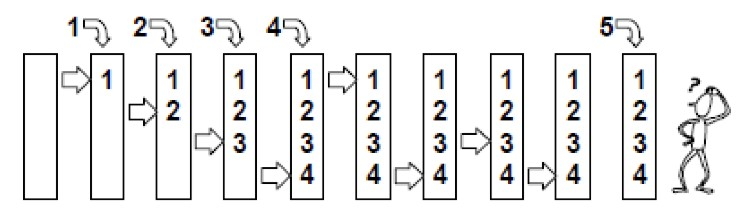
\includegraphics[scale=0.4]{paging/paging-1.jpg}
    \end{center}

    Na kolejnych rysunkach pokazany jest stan poszczególnych ramek,
    zależnie od zastosowanego algorytmu. Przy okazji pokazane jest
    odniesienie do pamięci, które spowoduje kolejny błąd błąd strony i
    tym samym problem zastępowania. Usunięcie tej samej strony w
    przypadku algorytmów LFU i LRU oraz MFU i LIFO jest przypadkowe
    i kolejna wymiana w przypadku tych algorytmów może wykazać
    różnice.
    Warto też przy tej okazji zwrócić uwagę, że dla algorytmów
    licznikowych wybór może być niejednoznaczny, gdyż liczba
    odniesień do różnych stron może być taka sama. Jako kryterium
    rozstrzygnięcia można przyjąć czas sprowadzenia, czyli strony z taką
    samą wartością licznika usuwane są w kolejności FIFO. Przy
    założeniu, że strony sprowadzane są pojedynczo nie ma tego
    problemu w algorytmach opartych na kolejności zdarzeń w czasie,
    czyli MIN, FIFO, LIFO i LRU.

    \begin{center}
        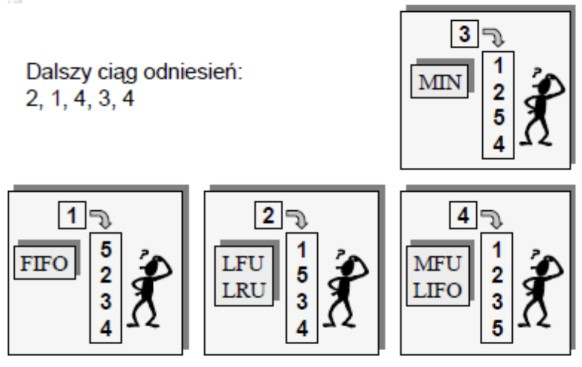
\includegraphics[scale=0.4]{paging/paging-2.jpg}
    \end{center}

    \newpage

    \section{Systemy plikowe - organizacja fizyczna i logiczna (na przykładzie wybranego systemu uniksopodobnego).}

    \subsection{Organizacja fizyczna}
    \begin{itemize}
        \item Przydział miejsca na dysku
        \begin{itemize}
            \item Przydział ciągły (ang. contiguous allocation) — cały plik zajmuje ciąg kolejnych bloków
            \item Przydział listowy (łańcuchowy, ang. linked allocation, chained allocation) — bloki pliku tworzą listę powiązaną
            \item Przydział indeksowy (ang. indexed allocation) — bloki z danymi wskazywane są przez bloki indeksowe, które mogą być
            zorganizowane w:
            \begin{itemize}
                \item schemat listowy
                \item schemat wielopoziomowy
                \item schemat kombinowany
            \end{itemize}
        \end{itemize}
        \item Zarządzanie wolną przestrzenią
        \begin{itemize}
            \item Wektor bitowy — każdy bit odpowiada jednemu blokowi, wartość 1 oznacza wolny blok.
            \item Lista powiązana — każdy wolny blok zawiera indeks następnego wolnego bloku.
            \item Grupowanie — niektóre wolne bloki zapełnione są w całości indeksami innych wolnych bloków, ostatni indeks wskazuje na
            kolejny blok zapełniony w całości indeksami.
            \item Zliczanie — wykaz wolnych bloków obejmuje indeks pierwszego wolnego bloku oraz liczbę wolnych bloków znajdujących się za
            nim, stanowiących ciągły obszar.
        \end{itemize}
        \item Implementacja katalogu – lista liniowa, tablica haszowa, struktura indeksowa
    \end{itemize}

    \subsection{organizacja logiczna}
    \subsubsection{Zadania systemu operacyjnego}
    Zadaniem systemu operacyjnego w odniesieniu do plików jest zapewnienie odwzorowania pomiędzy abstrakcyjnym obrazem
    informacji a jego reprezentacją na urządzeniu fizycznym.
    \begin{itemize}
        \item identyfikacja pliku (hierarchiczna struktura katalogów)
        \item udostępnienie interfejsu operacji plikowych (API)
        \item realizacja operacji dostępu do plików i katalogów z zapewnieniem bezpieczeństwa (synchronizacja i autoryzacja dostępu),
        spójności i efektywności
    \end{itemize}

    \subsubsection{Atrybuty pliku}
    \begin{itemize}
        \item Nazwa — ciąg znaków służących użytkownikowi do identyfikacji pliku
        \item Typ — informacja służąca do rozpoznania rodzaju zawartości pliku i tym samym sposobu interpretacji
        \item Lokalizacja — informacja służąca do odnalezienia pliku w systemie komputerowym (urządzenie i położenie pliku w tym
        urządzeniu)
        \item Rozmiar — bieżący rozmiar pliku w ustalonych jednostkach (bajtach, słowach, blokach itp.)
        \item Ochrona — informacje umożliwiające kontrolę dostępu
        \item Czasy dostępów — daty i czasy wykonywania pewnych operacji na pliku, typu odczyt, modyfikacja, utworzenie
    \end{itemize}

    \subsubsection{Struktura pliku}
    Logiczna struktura pliku określa powiązanie informacji wewnątrz pliku (właściwym byłoby zatem określenie struktura informacji).
    Jako przykład można sobie wyobrazić plik z tabelą bazy danych, w którym:
    \begin{itemize}
        \item pierwsze 4 bajty określają liczbę rekordów (krotek),
        \item następne 2 — długość rekordu w bajtach,
        \item kolejny bajt — długość nagłówka z definicją atrybutów,
        \item reszta przeznaczona jest na dane, przy czym każdy rekord ma dodatkowo 2 bajty kontrolne.
    \end{itemize}
    Z długości nagłówka wynika, gdzie rozpoczynają się dane, z wielkości rekordu oraz informacji o strukturze, mówiącej o 2
    dodatkowych bajtach dla każdego rekordu, można wyliczyć początek rekordu o podanym numerze itd.

    \subsection{UNIX}
    \subsubsection{Informacje ogólne}
    \begin{itemize}
        \item Z każdym plikiem związany jest i-węzeł, który przechowuje wszystkie atrybuty pliku z wyjątkiem nazwy.
        \item Nazwa znajduje się w katalogu obok numeru i-węzła danego pliku.
        \item Katalogi tworzą strukturę wielopoziomową (katalog zawiera wpis specyfikujący inny katalog).
        \item Dane (zawartość pliku) znajdują się w blokach (jednostkach alokacji) o ustalonym rozmiarze.
        \item Bloki danych identyfikowane są za pośrednictwem indeksu kombinowanego.
        \item Wolne bloki zorganizowane są zgodnie z zasadą grupowania.
    \end{itemize}

    Podstawą implementacji jest iwęzeł, grupujący wszystkie
    atrybuty pliku z wyjątkiem nazwy. I-węzły tworzą tablicę, której rozmiar limituje liczbę plików w systemie. I-węzeł pośrednio lub
    bezpośrednio identyfikuje bloki danych pliku. Wolna przestrzeń jest identyfikowana przez grupowanie, przy czym pierwszy węzeł
    (blok) z indeksami wolnych bloków zlokalizowany jest w całości w bloku nadrzędnym. W pewnych odmianach stosowany jest
    wektor bitowy. Wektor bitowy w tych odmianach używany jest również do identyfikacji wolnych i-węzłów.

    \subsubsection{Format partycji}
    Dwa główne element partycji stanowią: tablica i-węzłów oraz bloki danych. Liczba i-węzłów jest ustalona, podobnie jak liczba bloków danych. Ograniczenia na rozmiar katalogu wynikają wyłącznie z dostępności bloków danych, gdyż katalog zajmuje przestrzeń dyskową na takich samych
    zasadach, jak plik. Jego zawartość jest jednak interpretowana przez system zgodnie z zasadami budowy katalogów w danej
    implementacji. Jeden, ustalony i-węzeł opisuje korzeń drzewa katalogów.

    \subsubsection{Fizyczna struktura pliku}
    Z każdym plikiem związany jest 1 i-węzeł. Zawiera
    on podstawowe atrybuty pliku w modelu
    uniksowym, czyli:
    \begin{itemize}
        \item identyfikator właściciela i grupy,
        \item typ pliku — plik zwykły, katalog, dowiązanie
        symboliczne, łącze nazwane, urządzenie znakowe,
        urządzenie blokowe, gniazdo,
        \item prawa dostępu — tradycyjne rwx dla właściciela,
        grupy i pozostałych,
        \item czasy dostępu — czas modyfikacji pliku, czas
        modyfikacji i-węzła, czas dostępu,
        \item licznik dowiązań — liczba różnych nazw, pod
        jakimi występuje plik w systemie,
        \item rozmiar w bajtach.
    \end{itemize}

    Pozostała część i-węzła wypełniona jest indeksami
    bloków z danymi. Część indeksów w i-węźle (10 –
    12, zależnie od odmiany) wskazuje bezpośrednio
    bloki z danymi. Ponadto są jeszcze 3 indeksy, z
    których jeden wskazuje blok indeksowy 1-
    poziomowy, jeden — blok indeksu 2-poziomowego,
    a jeden — blok indeksu 3-poziomowego.

    \subsubsection{Struktura wpisu katalogowego}
    Katalog składa się z wpisów, kojarzących nazwę z i-węzłem. W tradycyjnym podejściu nazwa
    ograniczona była do 14 znaków, ale oczywiście w toku rozwoju systemów uniksowych
    wielkość tę zwiększano i współcześnie dopuszcza się nawet 256 znaków. W katalogu istnieją
    też wpisy specjalne o nazwie . (kropka) i .. (dwie kropki), skojarzone z numerem i-węzła
    odpowiednio katalogu bieżącego i nadrzędnego. Wyjątkiem w tym zakresie jest korzeń drzewa
    katalogów, który nie ma nadkatalogu.

    \newpage

    \section{Model ISO OSI. Przykłady protokołów w poszczególnych warstwach.}
    Model OSI (Open Systems Interconnection) utworzony przez Międzynarodową Organizację Normalizacyjną ISO stanowi
    \textbf{model referencyjny}.

    \begin{table}[H]
        \begin{center}
            \begin{tabular}{|c|c|c| }
                \hline
                \textbf{Nr warstwy OSI} & \textbf{Nazwa warstwy OSI} & \textbf{Przykładowe protokoły}\\
                \hline
                \hline
                7 & Aplikacji & HTTP, HTTPS, DNS, Telnet\\
                \hline
                6 & Prezentacji & SSL, TSL\\
                \hline
                5 & Sesji & NetBios, SAP\\
                \hline
                4 & Transportu & TCP, UDP\\
                \hline
                3 & Sieci & IPv4, IPv6, IGMP\\
                \hline
                2 & Łącza danych & ARP\\
                \hline
                1 & Fizyczna & Ethernet\\
                \hline
            \end{tabular}
        \end{center}
    \end{table}

    \noindent \textbf{Warstwa aplikacji} - interfejs między aplikacjami a
    usługami sieci.
    \begin{itemize}
        \item \textbf{HTTP/HTTPS} (Hypertext Transfer Protocol (Secure)) - protokół przesyłania dokumentów hipertekstowych.
        \item \textbf{DNS} (Domain Name System) - hierarchiczny rozporszony sytem nazw sieciowych, który odpowiada na zapytania
        o nazwy domen.
        \item \textbf{Telnet} - protokół do obsługi odległego terminala w architekturze klient-serwer.
    \end{itemize}

    \noindent \textbf{Warstwa prezentacji} - kompresja, kodowanie i
    translacja między niezgodnymi schematami kodowania oraz szyfrowanie.
    \begin{itemize}
        \item \textbf{SSL} (Secure Socket Layer) - protokół szyfrowania zapewniający poufność i ingtegralność danych.
        Otwarty protokół umożliwiający autoryzację serwerów i klientów, wykorzystuje szyfrowanie symetryczne
        z kluczem publicznym, stosuje sumy kontrolne dla zapewnienia integralności danych.
        \item \textbf{TSL} (Transport Layer Security) - jak wyżej. Ustalenie klucza symetrycznego szyfrowaniem niesymetrycznym,
        symetryczne szyfrowanie danych.
    \end{itemize}

    \noindent \textbf{Warstwa sesji} - zarządzanie przebiegiem komunikacji podczas
    połączenia między komputerami.
    \begin{itemize}
        \item \textbf{NetBios} (Network Basic Input/Output System) - protokół sieciowy zapewniający podstawowy interfejs
        łączenia aplikacji z innymi aplikacjami w sieci lokalnej.
        \item \textbf{SAP} (Session Announcement Protocol) - protokół wykorzystywany przez usługi powodujące tzw.
        ``burze rozgłoszeń'' (radio, telewizja internetowa).
    \end{itemize}

    \noindent \textbf{Warstwa transportu} - kontrola błędów i przepływu danych
    poza lokalnymi segmentami LAN, protokoły zapewniające
    komunikację procesów uruchomionych na odległych komputerach, protokoły TCP, UDP.
    \begin{itemize}
        \item \textbf{TCP} (Transmission Control Protocol) - połączeniowy, niezawodny, strumieniowy protokół komunikacyjny
        stosowany do przesyłania danych pomiędzy procesami na różnych maszynach.
        \item \textbf{UDP} (User Datagram Protocol) - prosty bezpołączeniowo protokół komunikacyjny, nie zapewnia
        niezawodności.
    \end{itemize}

    \noindent \textbf{Warstwa sieci} - określenie trasy przesyłania
    danych między komputerami poza lokalnym segmentem sieci LAN, protokoły trasowane takie jak IP (ze stosu protokołów TCP/IP).
    \begin{itemize}
        \item \textbf{IP} (Internet Protocol) - protokół internetowy będący zbiorem kroków
        postępowania wykonywanych automatycznie przez urządzenie w celu nawiązania łączności.
        \item \textbf{IGMP} (Internet Group Managament Protocol) - protokół internetowy służacy do zarządzania
        grupami multicastowymi w sieciach opartych na protokole IP.
    \end{itemize}

    \noindent \textbf{Warstwa łącza danych} – grupowanie danych wejściowych (z warstwy fizycznej) w bloki zwane \textbf{ramkami} danych („jednostki
    danych usług warstwy fizycznej”), mechanizmy kontroli poprawności
    transmisji (FCS).
    \begin{itemize}
        \item \textbf{ARP} (Address Resolution Protocol) - protokół sieciowy umożliwiający mapowanie logicznych
        adresów warstwy sieciowej na fizyczne adresy warstwy łącza danych (np. mapowanie IP na MAC).
    \end{itemize}

    \noindent \textbf{Warstwa fizyczna} - standard połączenia fizycznego, charakterystyki wydajnościowe nośników. Same media transmisyjne pozostają poza dziedziną jej
    zainteresowania (czasem określane są terminem warstwa zerowa).
    \begin{itemize}
        \item \textbf{Ethernet} - technologia zawierająca specyfikację przewodów, sygnałów, ramek.
        \item \textbf{DSL} (Digital Subsriber Line) - technologia cyfrowego szerokopasmowego dostępu do Internetu.
    \end{itemize}

    \newpage

    \section{Adresowanie w protokołach IPv4 i IPv6.}

    \subsection{Adresowanie w IPv4.}
    Adres IP jest przypisywany do karty sieciowej, nie do komputera. Składają się z czterech części bo 8 bajtów\\

    \noindent Istnieją \textbf{trzy typy adresów IPv4}:
    \begin{itemize}
        \item \textbf{Adresy jednostkowe} (unicast) – pojedynczy interfejs sieciowy (one-to-one).
        \item \textbf{Adresy rozgłoszeniowe} (broadcast) – wszystkie węzły w tym samym segmencie sieci (one-to-everyone).
        \item \textbf{Adresy grupowe} (multicast) – jeden lub wiele komputerów w jednej lub w różnych segmentach sieci (one-to-many).
    \end{itemize}

    \noindent W \textbf{adresie IP} zapisanym binarnie można wyróżnić \textbf{dwie części}:
    \begin{itemize}
        \item \textbf{Identyfikator sieci} (Network ID) - pewna liczba bitów z lewej strony adresu.
        \item \textbf{Identyfikator hosta} (Host ID) - pozostałe bity.
    \end{itemize}
    \textbf{Granica} między identyfikatorem sieci a identyfikatorem hosta może być wyznaczona przez
    tzw. \textbf{maskę sieci}.

    Adres IP, który zawiera \textbf{same zera} w części hosta jest traktowany jako \textbf{adres sieci}.
    \textbf{Adresy rozgłoszenia do sieci lub podsieci mają jedynki tylko w części hosta}.

    \textbf{Adres ograniczonego rozgłoszenia} - 255.255.255.255- adres rozgłoszenia
    w danym segmencie sieci ograniczonym routerami.\\

    \subsubsection{Adresowanie oparte na klasach}

    Pierwszy bajt adresu determinuje do jakiej klasy należy sieć.

    \begin{tabular}{|c|c|c|c|c|}
        \hline
        Klasa & Adres sieci & Adresy & Zakres 1-go bajtu & Najstarsze bity\\
        \hline
        A & w.0.0.0 & 1.0.0.0 - 126.0.0.0 & 1 – 126 & 0\\
        \hline
        B & w.x.0.0 & 128.0.0.0 - 191.255.0.0 & 128 – 191 & 10\\
        \hline
        C & w.x.y.0 & 192.0.0.0 - 223.255.255.0 & 192 – 223 & 110\\
        \hline
        D & nie dotyczy & nie dotyczy & 224 – 239 & 1110\\
        \hline
        E & nie dotyczy & nie dotyczy & 240 – 255 & 11110\\
        \hline
    \end{tabular}

    \begin{table}[H]
        \begin{center}
            \begin{tabular}{|c|c|c|c|c|c|c|}
                \hline
                Klasa & Ilość sieci & \# Hostów & ID sieci & ID hosta & pierwszy & ostatni\\
                \hline
                A & 126 & $2^{24}-2$ & 1 bajt & 3 bajty & w.0.0.1 & w.255.255.254\\
                \hline
                B & $(191-128+1)*256$ & $2^{16}-2$ & 2 bajty & 2 bajty & w.x.0.1 & w.x.255.254\\
                \hline
                C & $(192-223+1)*256^2$ & $2^8-2$ & 3 bajty & 1 bajt & w.x.z.1 & w.x.z.254\\
                \hline
            \end{tabular}
        \end{center}
    \end{table}


    \begin{itemize}
        \item \textbf{Adresy klasy D} - przeznaczone są do transmisji grupowych.
        \item \textbf{Adresy klasy E} - zarezerwowane (nie wykorzystywane normalnie do transmisji pakietów).
        \item \textbf{Adresy pętli zwrotnej} (loopback) - postaci 127.x.y.z (na ogół 127.0.0.1). Cały ruch przesyłany na ten adres nie wychodzi z komputera.
    \end{itemize}


    \subsubsection{Adresowanie bezklasowe}
    Dzielenie na podsieci z \textbf{użyciem dowolnej liczby jedynek}. Do określenia sieci należy podać adres
    sieci oraz maskę. Obecnie w Internecie powszechnie jest wykorzystywane adresowanie
    bezklasowe.

    \begin{itemize}
        \item Protokół \textbf{warstwy trzeciej} modelu ISO OSI.
        \item Oprogramowanie implementujące protokół IP jest odpowiedzialne za:
        \begin{itemize}
            \item \textbf{adresowanie} IP,
            \item \textbf{tworzenie datagramów} IP (pakietów)
            \item uczestniczenie w \textbf{kierowaniu ich} w sieci z punktu początkowego do punktu docelowego.
        \end{itemize}
        \item Realizuje usługę \textbf{zawodną}. Jeśli komunikacja powinna zawierać mechanizmy niezawodności, to muszą one być dostarczone przez protokoły warstwy wyższej.
        \item Datagram IP składa się z nagłówka (header) i bloku danych (payload).
        \begin{itemize}
            \item \textbf{Nagłówek} dzięki informacjom w nim zawartym umożliwia obsługę routowania, identyfikację bloku danych, określenie rozmiaru nagłówka i datagramu oraz obsługę fragmentacji. W nagłówku mogą się znaleźć również tzw. opcje rozszerzające.
            \item \textbf{Blok danych}.
        \end{itemize}
    \end{itemize}

    \subsection{Adresowanie w IPv6.}

    \begin{itemize}
        \item \textbf{osiem 16 bitowych sekcji w zapisie szesnastkowym}, oddzielonych dwukropkami,

        np.: fe80:0000:0000:0000:0202:b3ff:fe1e:8329
        \item długi ciąg zer może być \textbf{raz} połączony i przedstawiony jako dwa dwukropki "::"
        \item w środowisku z węzłami IPv4 oraz IPv6 często \textbf{w adresie IPv6 umieszcza się również IPv4}. Są dwa typy takich adresów:
        \begin{itemize}
            \item \textbf{Typ 1: IPv4-Compatible IPv6 Address} - 96 bitów zero + adres IPv4
            \item \textbf{Typ 2: IPv4-Mapped IPv6 Address} (zalecany) - $0000..............................0000$ ffff + IPv4 address
        \end{itemize}
        \item Zamiast identyfikatora sieci (jak było w IPv4), w IPv6 używa się tzw. \textbf{prefiksu}. Prefiks to \textbf{pewna liczba bitów} adresu licząc z lewej strony. Prefiks \textbf{określa} zatem \textbf{sieć}. Prefiks podaje się standardowo jako pewną liczbę sekcji adresu.
    \end{itemize}

    \subsubsection{Typy adresów}
    \begin{itemize}
        \item \textbf{Adres niewyspecyfikowany} - ::/128
        \item \textbf{Pętla zwrotna} (Loopback) - ::1/128
        \item \textbf{Multicast} - ff00::/8 (1111 1111)
        \item \textbf{Link-local unicast} - fe80::/10 (1111 1110 10)
        \item \textbf{Global unicast}
    \end{itemize}

    \subsubsection{Klasyfikacja adresów.}
    \begin{enumerate}
        \item \textbf{adresy jednostkowe (unicast)} - może być przypisany do wielu interfejsów w węźle lub wielu komputerów;
        podzielony na prefiks i identyfikator interfejsu, Typowy prefix - 48 bitów od dostawcy, 16 od podsieci.
        \item \textbf{adresy pobliskie (anycast)} - z zakresu adresów jednostkowych organizacji, przydzielane do grupy
        węzłów (np. routerów).
        \item \textbf{adresy grupowe (multicast)} - zastępują adresy rozgłoszeniowe i grupowe w IPv4, przydzielane do
        grupy węzłów lecz w przeciwieństwie do anycasta wszystkie węzły odbierają pakiety wysłane do danego adresu
        - 11111111 + 4 bity flagi + 4 bity zakresu + 112 bitów ID grupy.
    \end{enumerate}

    \subsubsection{Skąd wziąć adres MAC?}
    \begin{itemize}
        \item Unicastowy adres IP na multicastowy (Solicited Node Multicast address) - ff02:0:0:0:0:1:ff\_:\_ \_,
        z trzema najmłodszymi bajtami adresu IP
        \item Multicastowy MAC - 33:33:\_:\_:\_:\_ z czterema najmłodszymi bajtami adresu multicastowego
        \item Ramka skonstruowana z adresem MAC, z pakietem IP z multicastowym IP w środku, z unicastowym w komunikacie ICMP
        \item Switche się znają na tyle, że ramka w miarę dochodzi tylko tam gdzie trzeba
        \item Komputer otrzymujący ramkę sprawdza czy o niego chodzi w komunikacie ICMP, i unicastowo odpowiada
    \end{itemize}
    \newpage

    \section{Najważniejsze procesy zachodzące w sieci komputerowej od momentu wpisania adresu strony WWW do wyświetlenia strony w przeglądarce (komunikat HTTP, segment TCP, system DNS, pakiet IP, ARP, ramka).}
    W poniższych rozważaniach zakładamy, że klient wpisał w przeglądarkę internetową adres \texttt{www.ksi.sh}.
    Oto kolejne procesy, które dzieją się od wpisania tego adresu do wyświetlenia strony.
    \begin{enumerate}
        \item \textbf{Zapytanie DNS}
        \begin{enumerate}
            \item Przeglądarka internetowa uruchamia odpowiednie wywołanie systemowe odpowiedzialne za rozwiązanie nazwy domenowej na adres IP
            \item System operacyjny sprawdza, czy żądany adres nie jest zapisany w cache'u
            \item Jeżeli wpisu nie ma w cache'u wysyła on zapytanie do skonfigurowanego w systemie serwera DNS (najczęściej serwera naszego ISP - Internet Service Provider'a) o adres IP związany z domeną \texttt{www.ksi.sh}.
            Zapytanie to nazywamy \textbf{zapytaniem rekurencyjnym} - klient DNS przerzuca odpowiedzialność za znalezienie adresu IP na serwer DNS.
            \item Powyższy serwer DNS sprawdza, czy sam nie obsługuje żądanej domeny. Jeżeli tak, zwraca on adres IP szukanej domeny bezpośrednio ze swojej bazy.
            \item Powyższy serwer DNS sprawdza, czy zapytania o tę domenę również nie ma w cache'u
            \item Jeżeli serwer ten nie znajdzie odpowiedniego wpisu w swoim cache'u, rozpoczyna on serię \textbf{zapytań iteracyjnych} do \textbf{autorytatywnych} serwerów poszczególnych domen.
            \textbf{Serwer autorytatywny} to taki, który nie obsługuje rekurencyjnych zapytań od resolver'ów DNS (czyli np. zwykłych komputerów), a jedynie zapytania iteracyjne od innych serwerów o konkretne domeny.
            \item Przykładowy proces wyszukiwania iteracyjnego może wyglądać następująco:
            \begin{enumerate}
                \item Serwer DNS naszego ISP pobiera ze swojej konfiguracji adresy IP głównych serwerów DNS.
                Tych adresów IP jest 13, chociaż tak na prawdę, fizycznie tych serwerów jest oczywiście więcej
                - dzięki technice \texttt{anycast} wiele fizycznych serwerów jest widocznych pod tym samym adresem IP, a zapytanie na dany adres
                jest kierowane do najbliższego z nich względem pytającego.
                \item Serwer DNS naszego ISP wysyła zapytanie o domenę \texttt{www.ksi.sh} do jednego z głównych serwerów DNS
                \item Główny serwer DNS odpowiada mu, że nie wie jaki jest adres IP należący do \texttt{www.ksi.sh}, ale wie jaki serwer obsługuje domeny \texttt{sh} (jaki serwer jest serwerem autorytatywnym dla tej domeny)
                i zwraca on adres tego serwera
                \item Serwer DNS naszego ISP wysyła więc zapytanie do serwera autorytatywnego domeny \texttt{sh} o adres IP dla domeny \texttt{www.ksi.sh}
                \item Serwer obsługujący domenę \texttt{sh} odpowiada, że nie wie jaki jest adres IP dla \texttt{www.ksi.sh}, ale wie, jaki serwer obsługuje domenę \texttt{ksi.sh} i zwraca jego adres
                \item Serwer naszego ISP wysyła więc zapytanie o domenę \texttt{www.ksi.sh} do serwera autorytatywnego dla domeny \texttt{ksi.sh}
                \item Ten serwer z kolei okazuje się, że zna adres IP dla domeny \texttt{www.ksi.sh}, więc sprawdza go w swojej bazie danych i odsyła odpowiedź do serwera DNS naszego ISP
            \end{enumerate}
            \item Ostatecznie serwer DNS naszego ISP zapisuje znaleziony adres w swoim cache'u i odsyła go do naszego komputera z uruchomioną przeglądarką internetową
        \end{enumerate}

        \begin{center}
            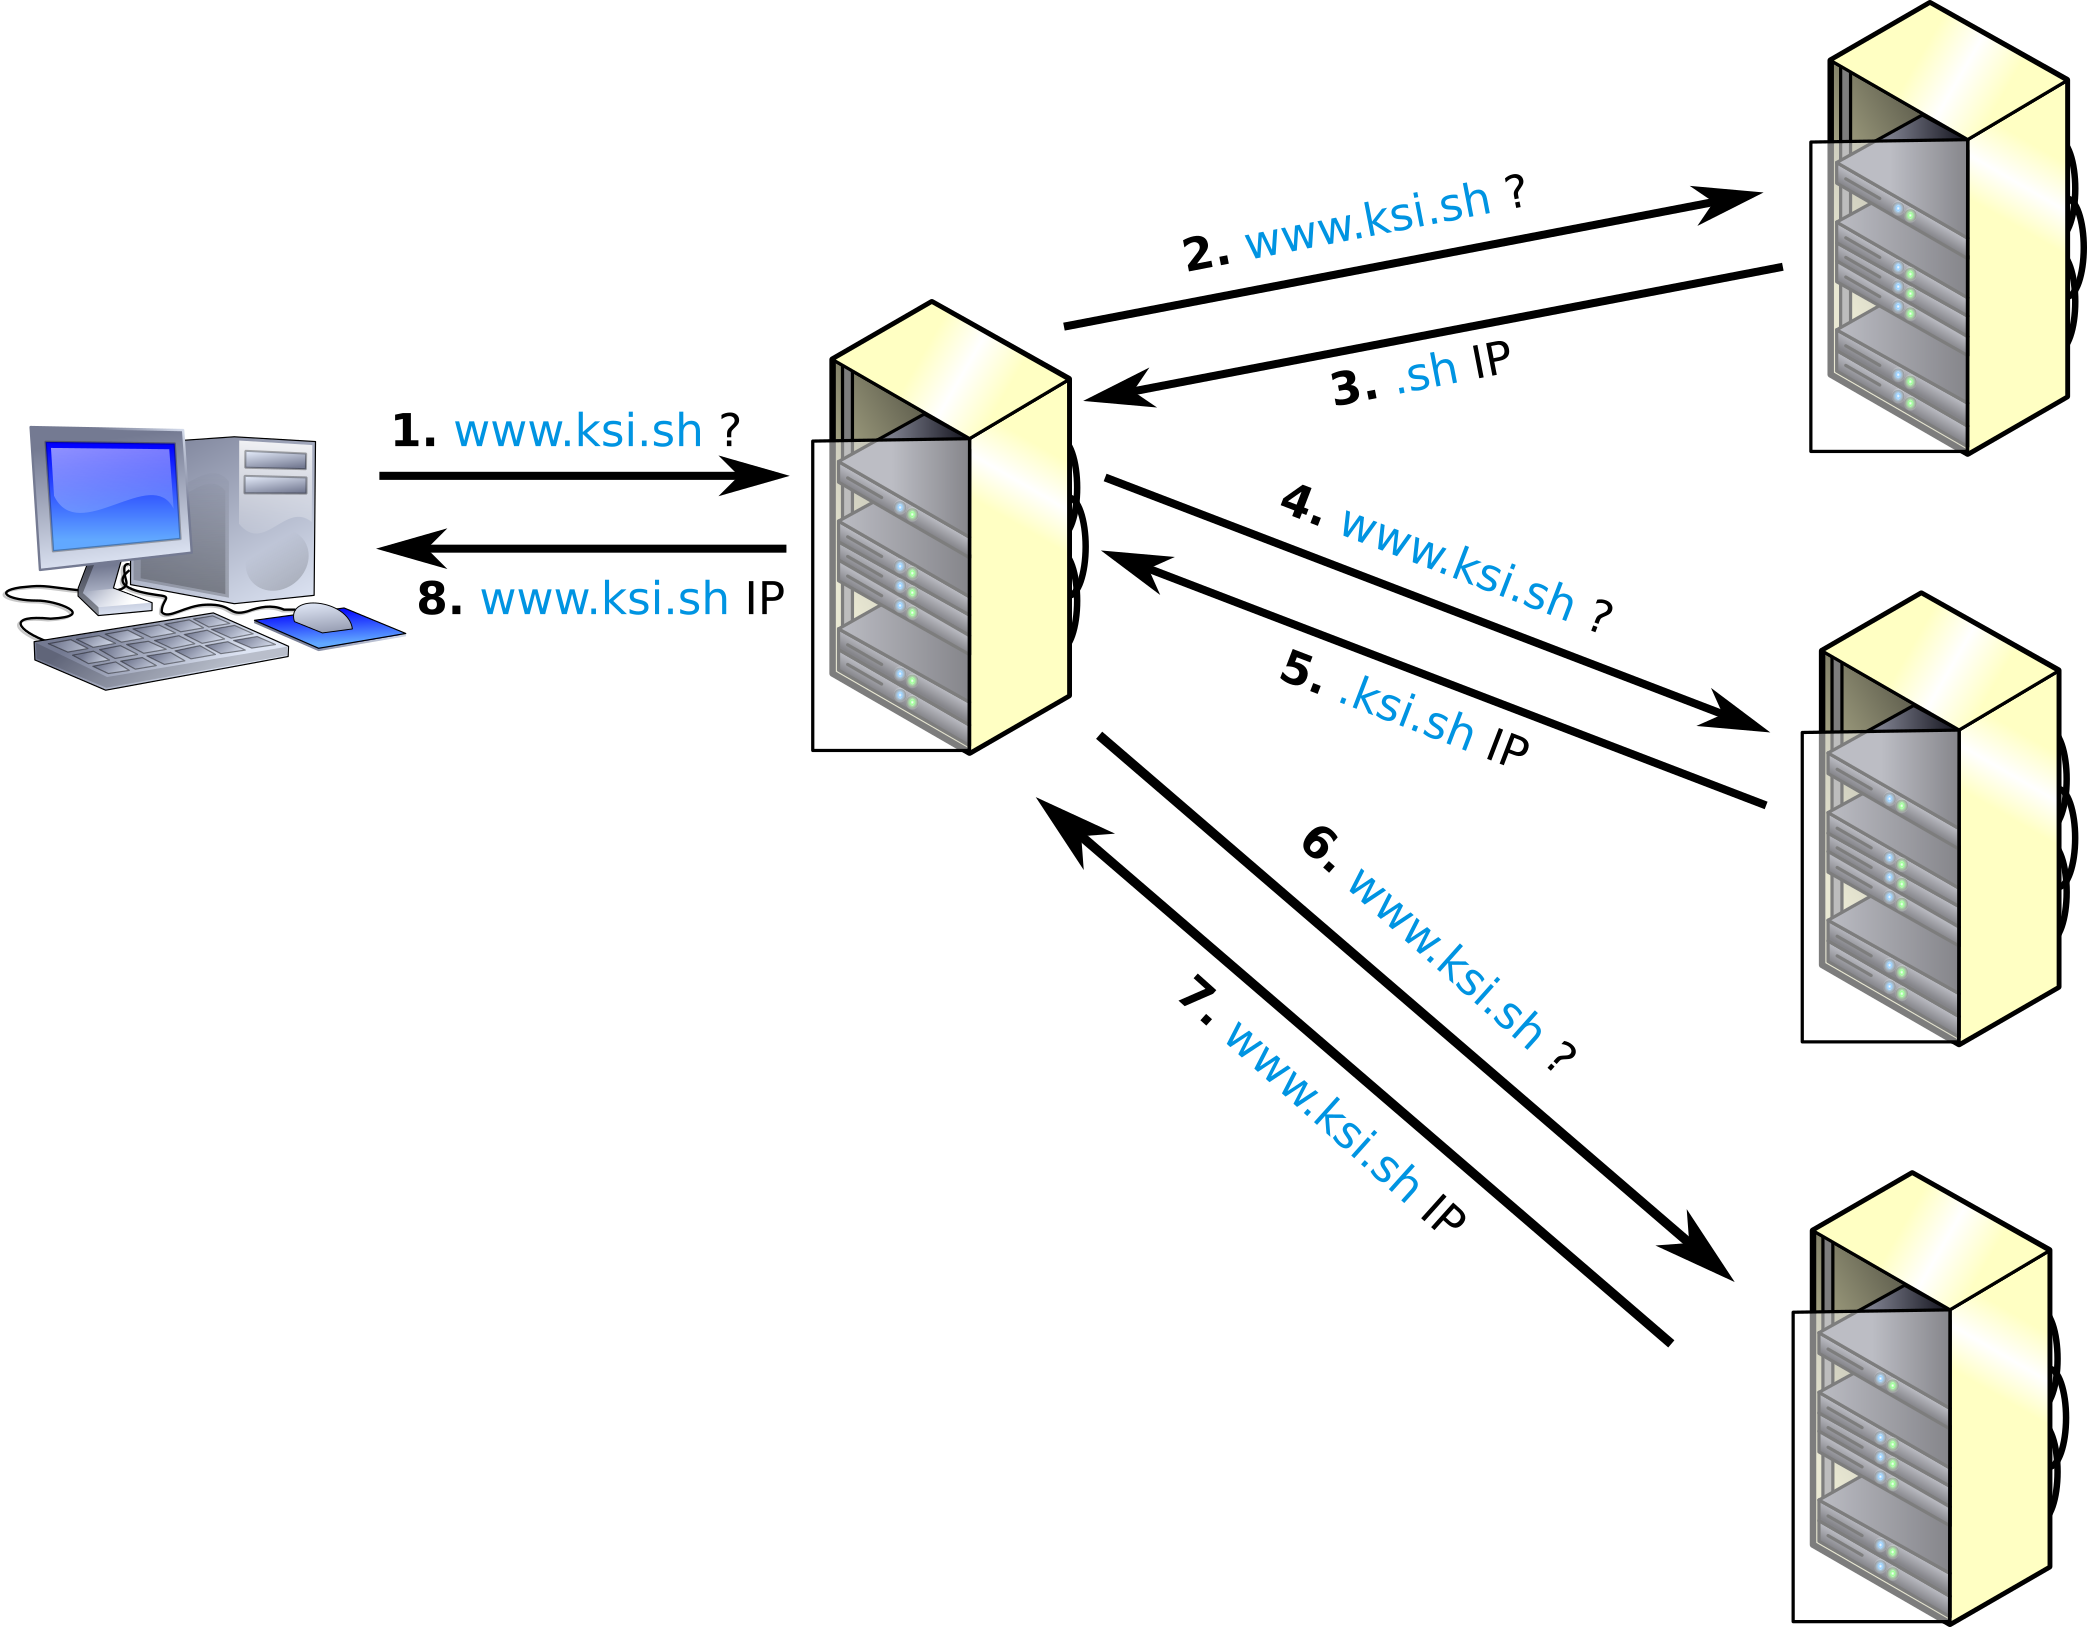
\includegraphics[width=\linewidth]{dns_resolving.png}
        \end{center}

        \item \textbf{Tworzenie pakietów zgodnie ze stosem TCP/IP}
        \begin{enumerate}
            \item Komputer z przeglądarką tworzy zapytanie HTTP o stronę \texttt{www.ksi.sh}
            \item Komputer tworzy \textbf{pakiet IP}:
            \begin{itemize}
                \item Adres źródłowy: adres IP komputera (jego adres w sieci LAN)
                \item Adres docelowy: adres serwera WWW otrzymany z zapytania DNS
                \item Port źródłowy: losowo wybrany spośród wolnych portów na lokalnym komputerze
                \item Port docelowy: specyficzny dla protokołu (w tym przypadku 80 lub 443 - chyba że w adresie URL podano inaczej)
            \end{itemize}
            i opakowywuje w ten pakiet zapytanie HTTP
            \item Komputer na podstawie swojego lokalnego adresu IP i ustawionej maski sprawdza, czy docelowy komputer znajduje się w jego sieci LAN.
            Załóżmy tutaj, że się nie znajduje.
            \item Komputer odczytuje więc ze swojej konfiguracji adres IP swojej bramy domyślnej
            \item Komputer musi dowiedzieć się teraz, jaki jest adres MAC odpowiadający adresowi IP bramy.
            W tym celu komputer sprawdza, czy nie ma go zapisanego w pamięci cache u siebie.
            Jeżeli nie, wysyła on na rozgłoszeniowy adres MAC (FF:FF:FF:FF:FF:FF) \textbf{ARP Request} - jest to zapytanie o to jaki adres MAC ma komputer o podanym adresie IP
            \item Komputer będący bramą odpowiada mu \textbf{unicastem} (na adres MAC naszego komputera) \textbf{ARP Response} - w ten sposób nasz komputer zna adres MAC bramy
            \item Komputer tworzy \textbf{ramkę}:
            \begin{itemize}
                \item Adres MAC źródłowy: adres MAC naszego komputera
                \item Adres MAC docelowy: adres MAC naszej bramy
            \end{itemize}
            i opakowywuje w tę ramkę pakiet IP
            \item Ramka następnie jest wysyłana (po uprzednim przetworzeniu na sygnały zgodne z medium, którym jest wysyłana - np. sygnały elektryczne) do sieci
        \end{enumerate}

        \item \textbf{Przekazywanie pakietów do serwera WWW i z powrotem}
        \begin{enumerate}
            \item Switch, do którego podłączony jest nasz komputer odbiera wysłane przez niego dane i zagląda do ramki
            \item Sprawdza on docelowy adres MAC i zgodnie ze swoją tablicą przełączania przekazuje tę ramkę na właściwy port
            lub w przypadku, gdy nie znajdzie odpowiedniego wpisu w swojej tablicy, rozsyła tę ramkę do wszystkich portów
            \item Po przejściu być może przez kolejne switch'e, które zachowują się tak samo, ramka trafia wreszcie do naszej bramy
            \item Brama jako router zagląda do pakietu IP i sprawdza zgodnie ze swoją tablicą routing'u
            (do której należą również bezpośrednio przyłączone do tego routera sieci) do jakiego kolejnego routera lub sieci skierować ten pakiet
            \item Gdy już znajdzie adres następnego skoku (kolejny router lub już komputer docelowy), router konstruuje kolejną ramkę do tego właśnie kolejnego routera
            lub komputera docelowego (wszystko dzieje się analogicznie, jak w przypadku konstruowania ramki przez komputer źródłowy), opakowuje w nią pakiet IP i wysyła
            \item Tak dzieje się do momentu aż pakiet nie dotrze do serwera WWW. Ten odczytuje żądanie HTTP, generuje odpowiedź HTTP i opakowuje ją w pakiet IP,
            w którym port źródłowy i docelowy oraz adres źródłowy i docelowy są zamienione ze sobą względem pakietu, który dostał - nadawca staje się odbiorcą
            \item Następnie serwer WWW tworzy ramkę (znów analogicznie jak to miało miejsce u klienta), w którą opakowuje wcześniej wspomniany pakiet i wysyła
            \item Wysłane przez serwer dane znów są przekazywane przez switch'e i router'y - tak jak to miało miejsce w przypadku wysłanego żądania od klienta do serwera,
            aż dojdą do naszego komputera (klienta)
            \item Ten z kolei odczytuje odpowiedź HTTP od serwera WWW i wyświetla zawartość strony
        \end{enumerate}
    \end{enumerate}
    \newpage

    \section{Działanie przełączników Ethernet, sieci VLAN, protokół STP.}
    \subsection{Działanie przełączników Ethernet}
    Przełącznik Ethernet'owy (Switch) w przeciwieństwie do Hub'ów nie rozsyła ramek, które do niego przyszły na wszystkie porty - co umożliwia łatwe podsłuchiwanie komunikacji,
    której nie jesteśmy odbiorcą oraz niepotrzebnie zwiększa ruch w sieci; lecz w zdecydowanej większości przypadków jest w stanie wysłać odebraną ramkę na jeden port,
    pod który jest podłączony jej odbiorca. Kieruje się on przy tym tablicą CAM (Content Addressable Memory – rodzaj tablicy asocjacyjnej), która jest swego rodzaju powiązaniem
    adresów MAC z portem (gniazdem) Switch'a, a którą uzupełnia na podstawie odbieranych ramek.
    Zasada działania Switch'a jest następująca:
    \begin{enumerate}
        \item Gdy switch odbiera na jakimś porcie ramkę, sprawdza on czy adresat (odbiorca), a właściwie jego adres MAC znajduje się w tablicy CAM:
        \begin{enumerate}
            \item Jeżeli tak - ramka wysyłana jest tylko na port powiązany z tym adresem MAC
            \item Jeżeli nie - Switch postąpi podobnie jak Hub - roześle tę ramkę do wszystkich portów. Podobnie postąpi, jeżeli adres MAC odbiorcy jest adresem broadcastowym
        \end{enumerate}
        \item Switch odczytuje z ramki adres MAC nadawcy i wiąże go z portem, na który przyszła ta ramka, oraz zapisuje tę informację w tablicy CAM
    \end{enumerate}

    \noindent Standardowe przełączniki warstwy drugiej mogą pracować w dwóch trybach pracy:
    \begin{enumerate}
        \item \textbf{Store-and-Forward} – przełącznik pobiera całą ramkę, analizuje czy nie jest błędna i przesyła ją dalej. Ten tryb wprowadza największe opóźnienie.
        \item \textbf{Cut-through} (dwa podtypy):
        \begin{enumerate}
            \item \textbf{Fast-forward switching} - po otrzymaniu adresu MAC miejsca docelowego ramki, już rozpoczyna się jej nadawanie.
            Jest to najszybsza metoda, ale nie sprawdza czy nie nastąpiła kolizja i ramka jest niepoprawna.
            \item \textbf{Fragment-free switching} - ramka jest przesyłana do portu docelowego dopiero po otrzymaniu 64 bajtów (rozmiar najmniejszej poprawnej ramki w Ethernecie).
            Zapewnia to, że ramka nie koliduje z inną
        \end{enumerate}
    \end{enumerate}


    \subsection{Sieci VLAN}
    W sieciach komputerowych często zachodzi potrzeba oddzielenia od siebie pewnej grupy komputerów tak, aby mogły one porozumiewać się między sobą w obrębie jednej grupy,
    ale jednocześnie, aby nie mogły się komunikować między grupami.
    Naturalnym rozwiązaniem wydaje się podłączenie grup do osobnych switch'y:

    \bigskip
    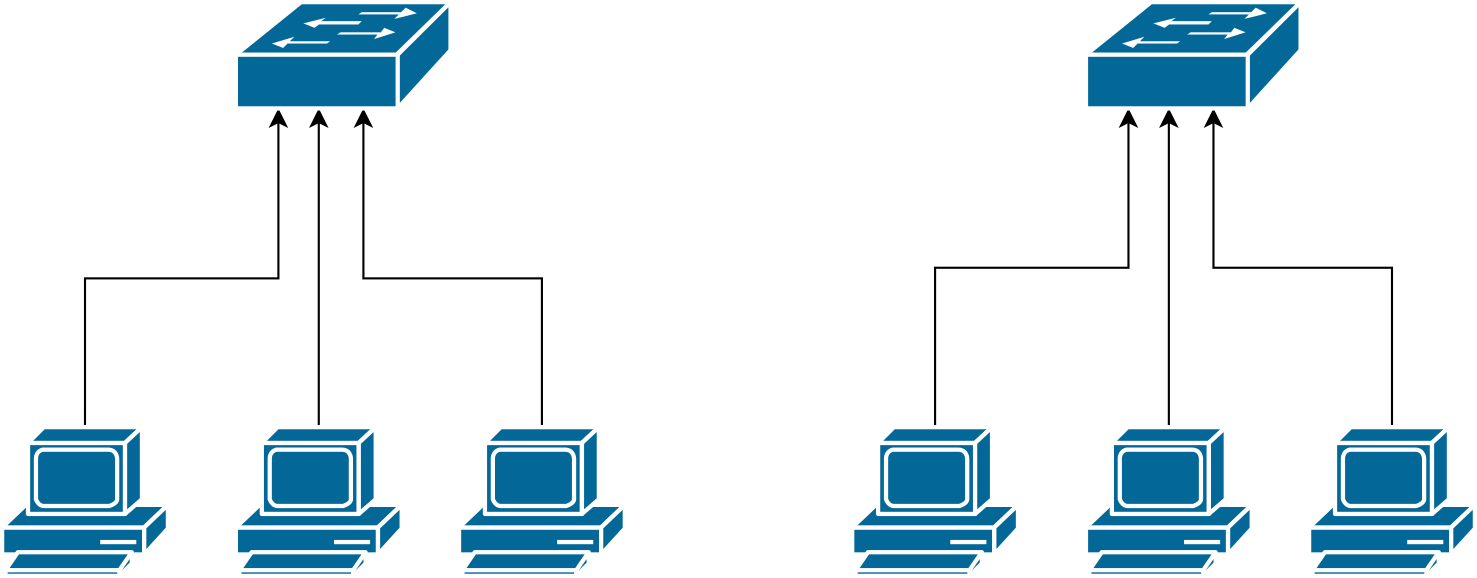
\includegraphics[width=\linewidth]{vlan/two_independent_switches.png}
    \smallskip

    \noindent Nie jest to jednak idealne rozwiązanie: dla każdej kolejnej grupy musimy kupować kolejne urządzenie, co przy większej ilości grup znacznie zwiększa koszty.
    Poza tym co jeżeli komputery z każdej z grup są np. na różnych piętrach? Musimy wtedy kupować kolejne urządzenia do obsługi komputerów na kolejnych piętrach oraz
    rozciągać między piętrami tak wiele kabli do połączeń między switch'ami, jak wiele mamy tych grup.

    Odpowiedzią na te potrzeby są \textbf{VLAN}'y (Virtual LAN). Dzięki nim na jednym switch'u jesteśmy w stanie wydzielić wiele osobnych ``podswitch'y'':
    każdy port (gniazdo) w switch'u możemy przypisać do konkretnego VLAN'u - te, które są w tym samym VLAN'ie mogą się ze sobą komunikować (zachowują się jak podpięte
    do tego samego switch'a), natomiast niemożliwa jest bezpośrednia komunikacja między dwoma różnymi VLAN'ami (tak jak komunikacja między dwoma niepołączonymi ze sobą switch'ami):

    \bigskip
    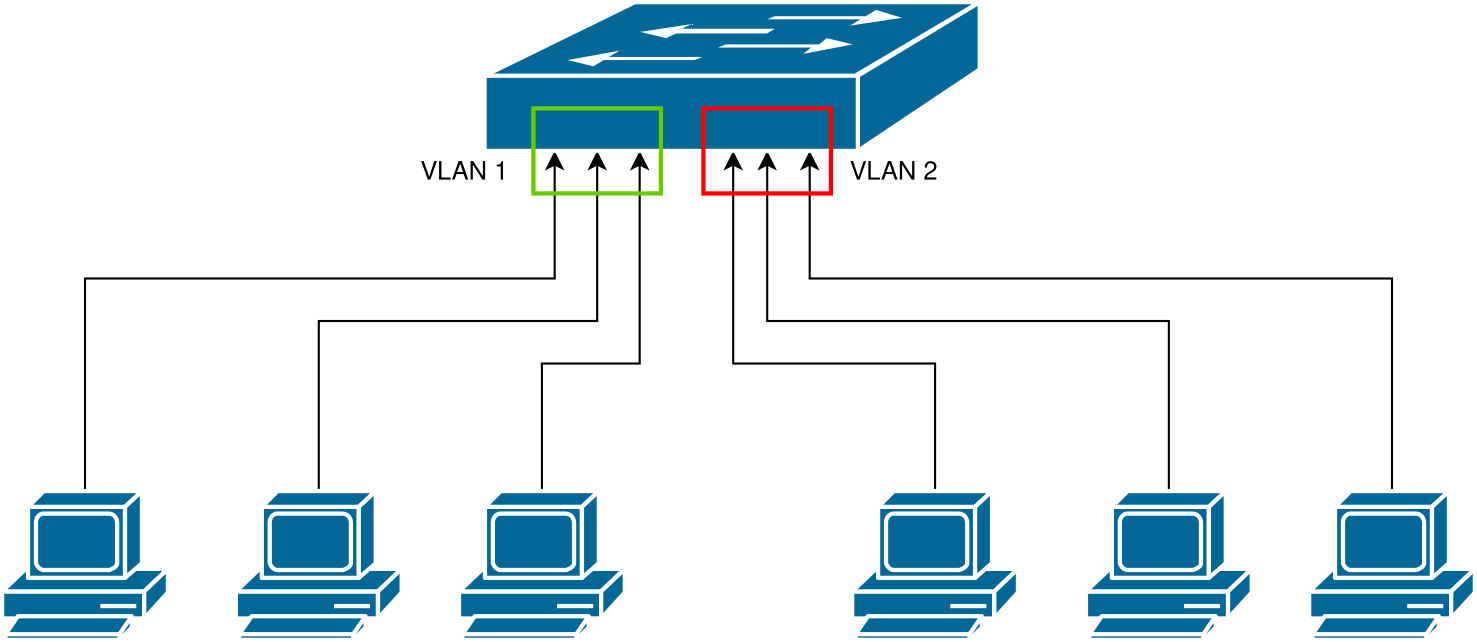
\includegraphics[width=\linewidth]{vlan/one_switch_two_vlans.png}
    \smallskip

    \noindent Daje to nam dużą swobodę:
    \begin{itemize}
        \item Nie musimy fizycznie przełączać kabli, gdy chcemy zmienić grupę dla danego komputera
        \item Utworzenie kolejnej grupy nic nas nie kosztuje - po prostu tworzymy kolejny VLAN i przypisujemy do niego odpowiednie porty
        \item Jednym kablem możemy przesyłać wiele VLAN'ów - nie potrzebujemy rozciągać wielu kabli między switch'ami na różnych piętrach (patrz dalej)
    \end{itemize}

    Ramki w przypadku technologi VLAN mogą być \textbf{tagowane} lub \textbf{nietagowane}. Te drugie to po prostu zwykłe ramki używane do tej pory w sieciach Ethernet.
    Ramki tagowane natomiast mają w sobie dodatkową informację do którego VLAN'u należą.

    Porty i połączenia, na których wysyłane/odbierane są ramki nietagowane nazywamy \textbf{dostępowymi}, natomiast te, gdzie komunikacja odbywa się
    przy pomocy ramek tagowanych nazywamy \textbf{trunk}'owymi. Standardowo komputery rozumieją tylko ramki nietagowane.

    Ramki tagowane otwierają nam nowe możliwości: możemy przy pomocy jednego kabla przesyłać ramki z wielu sieci VLAN, co pozwala np. połączyć za pomocą tylko jednego kabla
    switch'e z różnych pięter w rozważanym na początku przypadku, gdy komputery z jednej grupy znajdują się na różnych piętrach. Switch'e połączone są wtedy ze sobą łączem
    \textbf{trunk}'owym, dzięki czemu wysyłają one między sobą ramki tagowane, więc wiedzą, do którego VLAN'u (do której grupy komputerów) skierować przychodzącą ramkę:

    \bigskip
    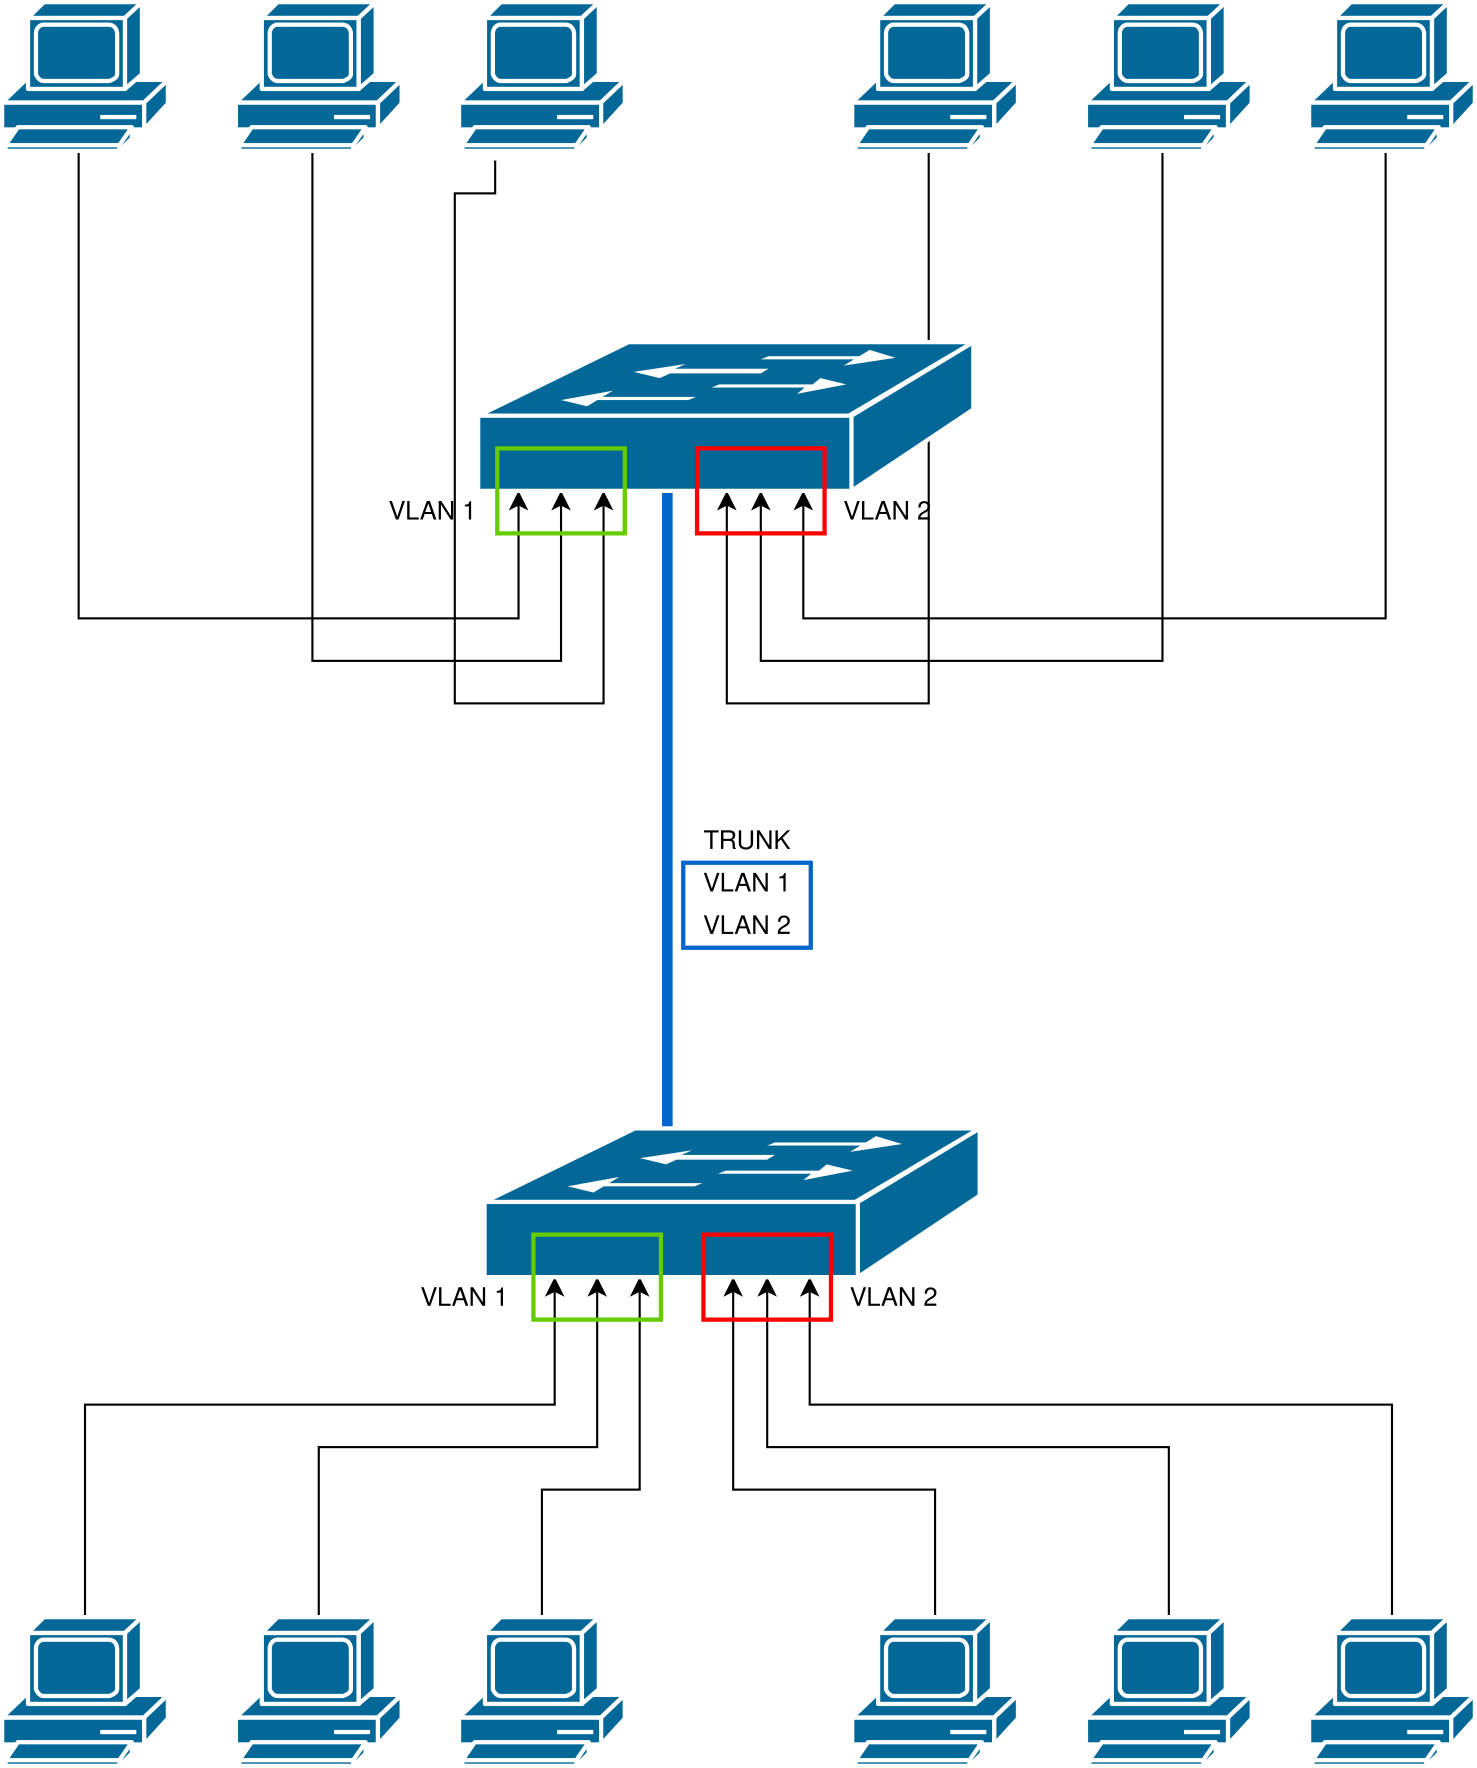
\includegraphics[width=\linewidth]{vlan/two_switches_with_trunk.png}
    \bigskip

    \newpage
    Czasami zachodzi jednak potrzeba, aby komputery mogły się ze sobą komunikować nawet między grupami (ale przeważnie chodzi nam o kontrolę takiej komunikacji
    - zezwolenie tylko na określony ruch). Ponieważ każdy VLAN traktowany jest jako osobna podsieć (w każdym z nich powinniśmy używać adresów IP z innej podsieci),
    aby umożliwić komunikację między VLAN'ami potrzebny nam jest \textbf{router}. Będzie on po prostu robił prosty routing między tymi sieciami, a dzięki zastosowaniu
    zasad na firewall'u będziemy mogli ograniczyć ten ruch tak, jak chcemy.

    Ponieważ router potrzebuje dostępu do wszystkich sieci VLAN, najprościej jest to osiągnąć poprzez podłączenie go do portu switch'a skonfigurowanego jako trunk.
    Takie podłączenie routera nazywamy \texttt{routerem na kiju} (router on a stick).
    Dzięki temu - podobnie jak w przypadku komunikacji między switch'ami będziemy mogli przy pomocy jednego kabla podłączyć do routera wiele sieci. Pomimo fizycznego
    podłączenia tylko do jednego interface'u routera, w praktyce dla każdego VLAN'u zostaną na nim utworzone \textbf{wirtualne interface}'y,
    które będą reprezentować poszczególne VLAN'y i to między nimi będzie wykonywany routing.

    Zauważmy, że w takiej konfiguracji, każdy ruch, który odbywa się między VLAN'ami musi przejść przez router. Może to znacznie zwiększyć obciążenie sieci:
    np. aby dwa komputery w różnych VLAN'ach jednak podłączone do tego samego switch'a mogły się ze sobą komunikować, cały ruch musi przejść niekiedy być może
    długą drogę przez całą sieć, aż do router'a i z powrotem. Aby temu zaradzić można użyć \textbf{Switch'y (przełączników) warstwy 3}. Są one mini routerami,
    które są w stanie wykonywać routing między VLAN'ami, które obsługują (z możliwością ustawienia zasad komunikacji między nimi - podobnie jak zasady firewall na routerze).
    Dzięki temu we wspomnianym wcześniej przykładzie ruch między tymi dwoma komputerami może odbywać się praktycznie tylko przy pomocy switch'a, do którego są podłączone
    - nie ma konieczności angażowania w to routera i innych switch'y.

    \bigskip
    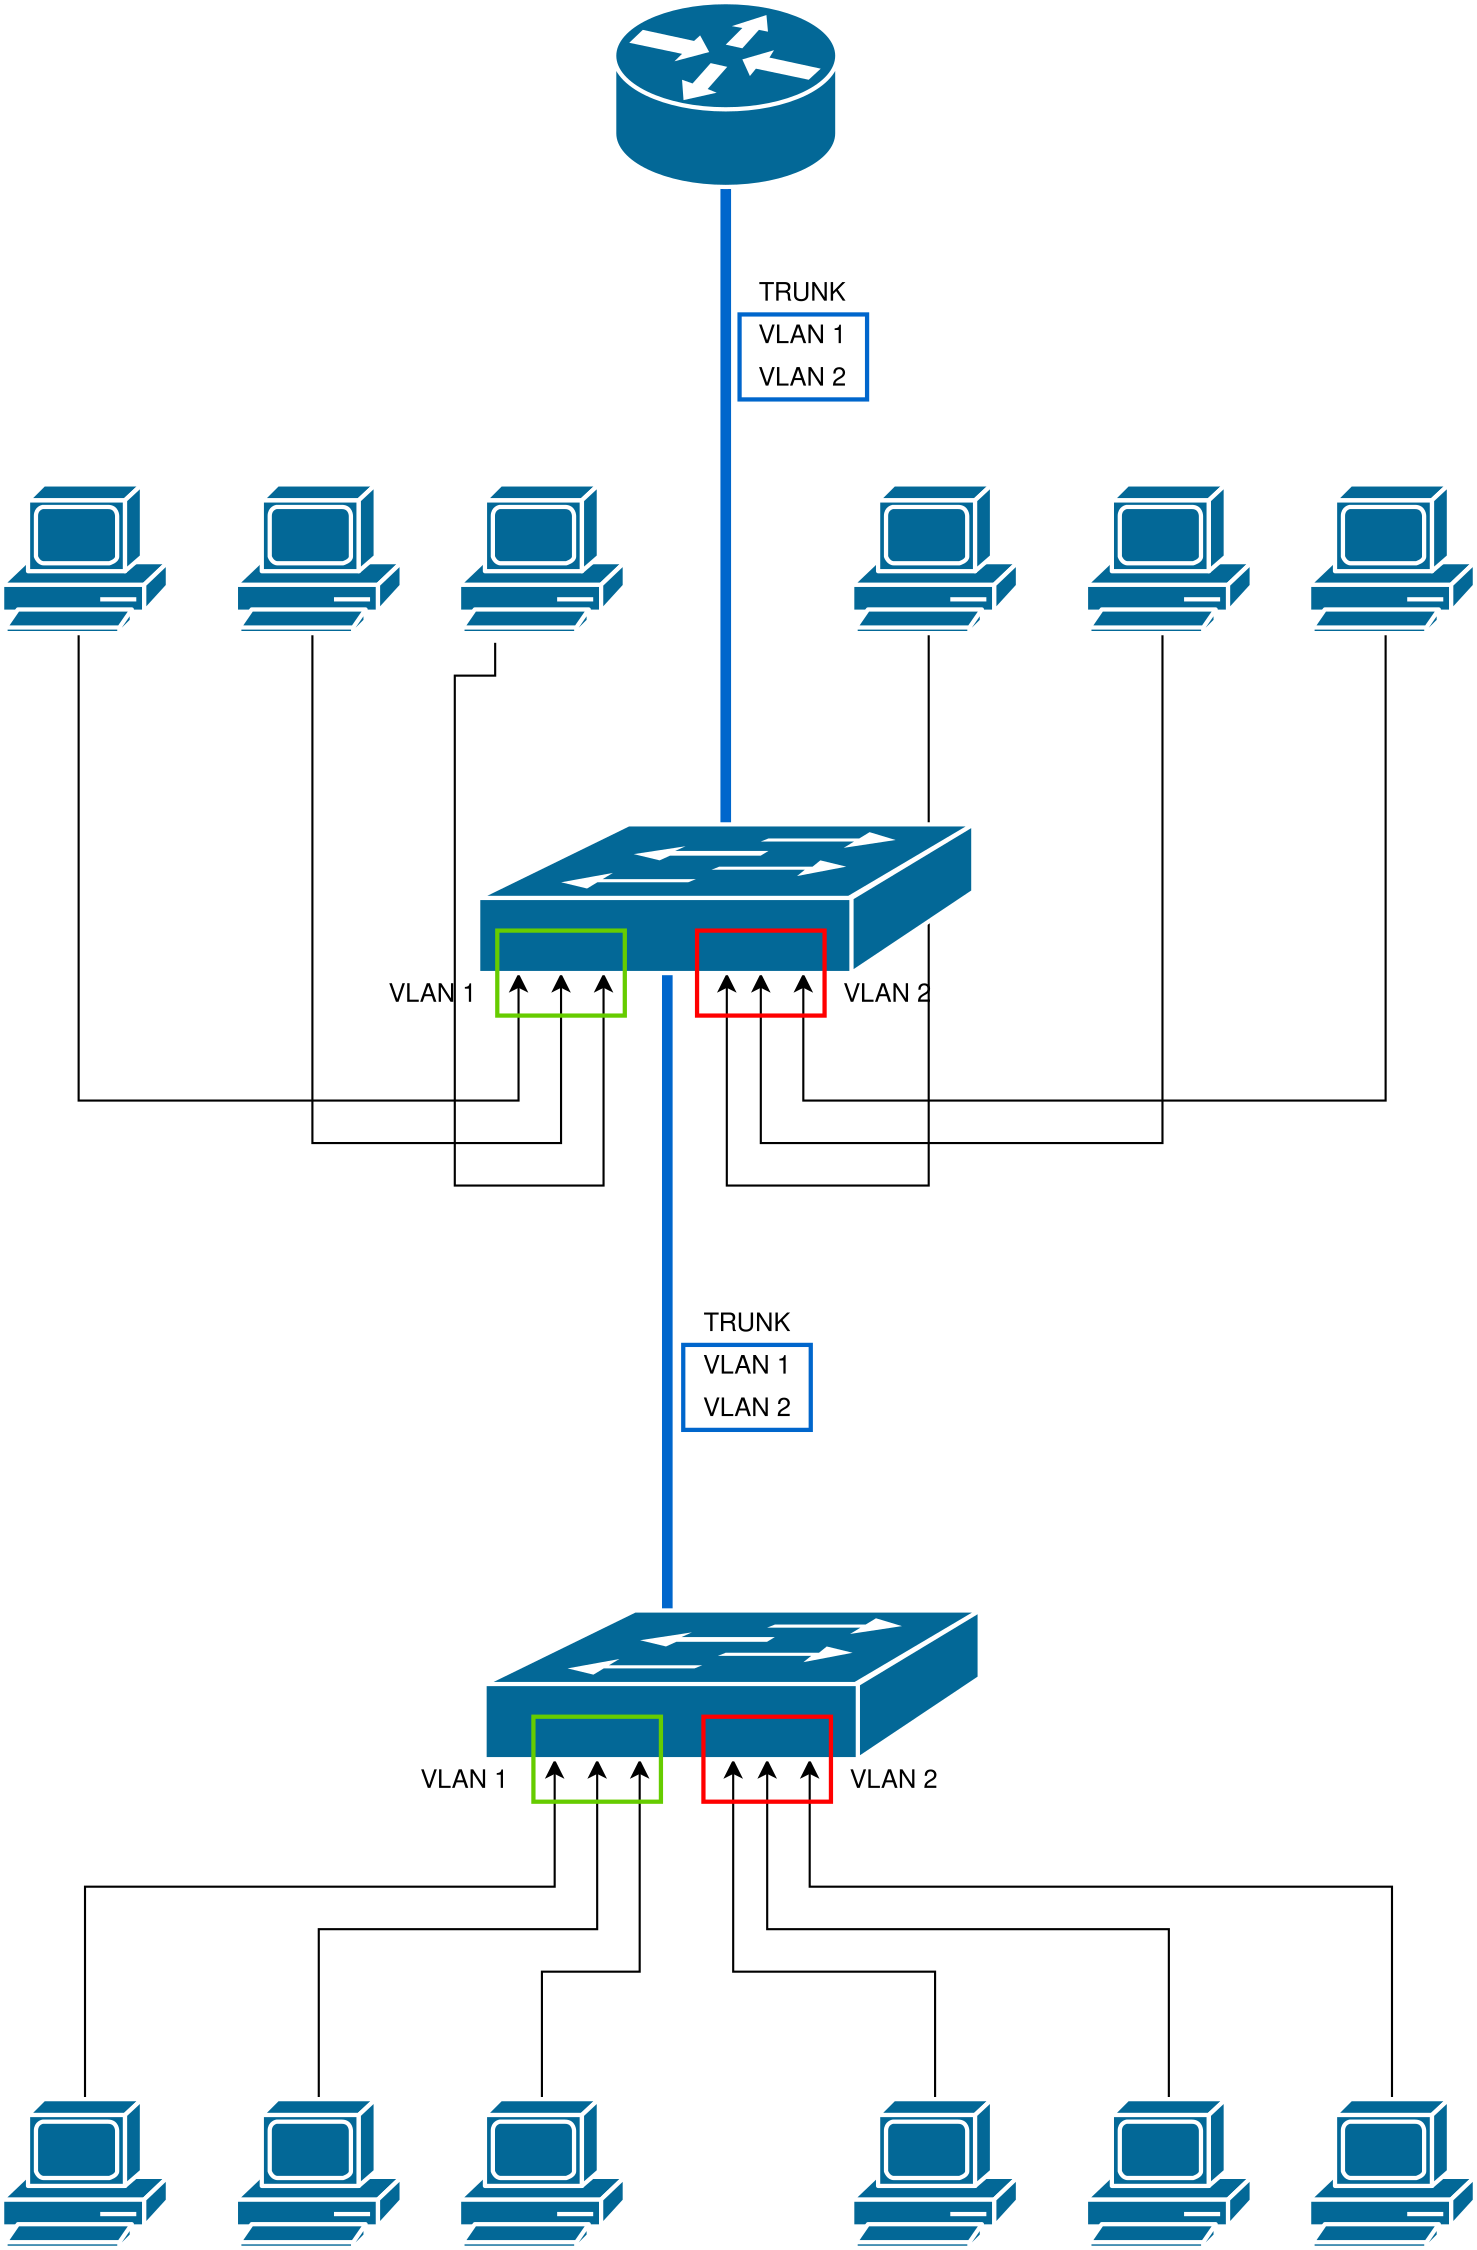
\includegraphics[width=\linewidth]{vlan/two_switches_and_router_with_trunk.png}


    \subsection{Protokół STP}
    \textbf{STP - Spanning-Tree Protocol} - jest protokołem umożliwiającym uniknięcie pętli w sieci LAN oraz mogącym zapewnić redundantne ścieżki komunikacji,
    które uaktywnią się w momencie awarii dotychczasowych.

    W nieco bardziej rozbudowanej sieci łączy się kilka lub więcej przełączników. Korzystnie jest,
    gdy przełączniki w sieci są połączone tak, by umożliwić zduplikowane ścieżki między nimi, ale
    żeby nie występowały pętle i niekorzystne zjawiska z nimi związane (burze rozgłoszeń w
    warstwie drugiej, dublowanie ramek, niestabilność zawartości tablicy CAM). Do realizacji
    tego celu służy protokół STP:

    \bigskip
    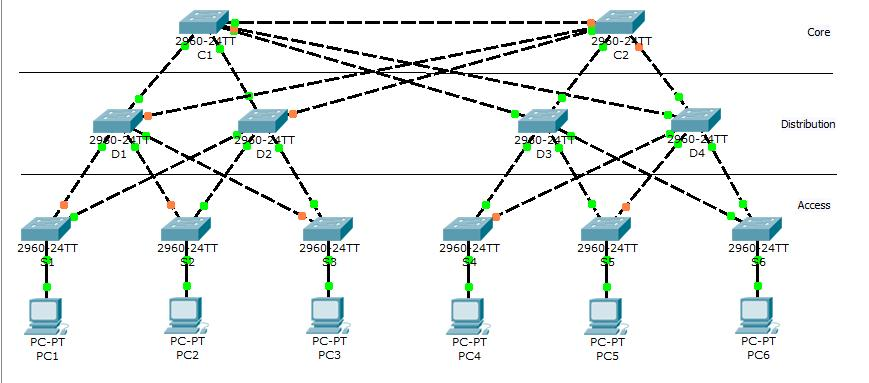
\includegraphics[width=\linewidth]{stp.png}
    \smallskip

    STP umożliwia tworzenie redundantnych ścieżek (połączeń) między przełącznikami, ale w
    danej chwili tylko jedno ze zduplikowanych połączeń jest aktywne. Aktywne połączenia
    tworzą strukturę drzewiastą z jednym przełącznikiem wybranym jako korzeń (root, root- switch lub root-bridge).
    STP powstał jak mosty były jeszcze powszechnie wykorzystywane i stąd w terminologii STP często zamiast switch mówi się bridge.

    STP wykorzystuje specjalne ramki BPDU (Bridge Protocol Data Units), które są regularnie
    przesyłane miedzy przełącznikami (np. co dwie sekundy). Ramki BPDU mają specjalny adres
    MAC docelowy typu multicast (01:80:C2:00:00:00) i są przesyłane według innych zasad jak
    zwykłe ramki: otrzymane ramki BPDU nie są wprost przekazywane do innych portów,
    przełącznik buduje swoje ramki BPDU uwzględniające otrzymane od innych informacje,
    takie jak np. koszt dotarcia do root-switch'a - powiększa go przed przesłaniem,
    podobnie jak w protokole routowania OSPF. \\

    \noindent Działanie STP:
    \begin{enumerate}
        \item \textbf{Wybór przełącznika-korzenia} (root-bridge) - jest realizowany na
        podstawie priorytetu przełącznika, który jest konfigurowalny. Jako korzeń wybierany
        jest przełącznik o najniższym priorytecie. Jeśli priorytety są jednakowe, to wybierany
        jest przełącznik o najniższym adresie MAC. Wybór korzenia drzewa rozpinającego jest
        realizowany z wykorzystaniem specjalnych ramek BPDU.
        \item \textbf{Wybór portów do korzeni} (root ports). Są to porty, którymi będą przekazywane ramki
        do przełącznika-korzenia. Port staje się zawsze „root-portem” jeśli jest bezpośrednio
        połączony do przełącznika – korzenia. Jeśli nie ma portów bezpośrednio dołączonych
        do korzenia, to jest analizowany koszt połączenia. Koszt ten jest zależny od szerokości
        pasma np. dla 10Mbps koszt wynosi 100, dla 100Mbps koszt
        wynosi 10, itd. Koszty są przekazywane w ramkach BPDU i
        przełączniki wyliczają całkowite koszty połączenia z przełącznikiem korzeniem – jako
        sumy kosztów poszczególnych połączeń. W każdym przełączniku port o najniższym
        koszcie trasy do przełącznika korzenia staje się root-portem (oczywiście tylko w
        przypadku, gdy w danym przełączniku nie ma bezpośredniego połączenia z
        przełącznikiem-korzeniem).
        \item \textbf{Wybór portów wyznaczonych} (designated ports). Są to porty, które uczestniczą
        w wymianie informacji w drzewie rozpinającym (spanning tree). Dla każdego
        segmentu sieci LAN jest określany jeden przełącznik wyznaczony (designated switch),
        przez który wiedzie normalna droga z danego segmentu do przełącznika-korzenia.
        Przykładowy segment sieci LAN: koncentrator połączony z dwoma przełącznikami
        oraz z pewną liczbą komputerów – hostów.
        \item \textbf{Blokada niepotrzebnych portów}. Po ustaleniu stanu połączeń wszystkie porty
        umożliwiające połączenia redundantne, a nie będące root-portami ani portami wyznaczonymi, są blokowane.
    \end{enumerate}

    Stan połączeń jest analizowany na podstawie ramek BPDU, które są przesyłane cyklicznie,
    standardowo co 2s (ten czas można zmienić). W przypadku uszkodzeń istniejących połączeń
    automatycznie odblokowywane są nowe porty, które przejmują przekazywanie ramek, ramki
    są zatem przesyłane nową trasą.

    \newpage

    \section{Rola routerów i podstawowe protokoły routingu (RIP, OSPF).}

    Sposób obsługi routowania przez warstwę IP nazywa się mechanizmem routowania.
    Określenie to dotyczy przeglądania przez system operacyjny tablicy routowania i podejmowania określonych decyzji, co do przesyłania datagramów IP.
    Przez pojęcie polityka routowania określa się działania procesu routowania podejmowane w
    celu ustanowienia i bieżącej modyfikacji tablicy routowania. Polityka routowania realizowana jest z wykorzystaniem protokołów routowania.

    Pożądane cechy protokołów routowania:
    \begin{enumerate}
        \item Wyznaczenie najlepszej trasy do punktu docelowego
        \item Odporność (robustness) na nieprzewidziane, nieporządanie zdarzenia:
        "kopara", niewłaściwa konfiguracja, obciążenia sieci
        \item Szybkie osiaganie zbieżności, tj. osiągnięcie stanu w którym
        routery "widzą" jednakowo topologię sieci.
        \item Dopasowanie do zmian, np.:
        \begin{itemize}
            \item Odłączenie danej sieci
            \item Podłączenie nowej sieci
            \item Zmiana szerokości pasma
            \item Zmiana opóźnienia
        \end{itemize}
    \end{enumerate}

    Ze względu na sposób działania protokoły routowania wewnętrznego dzielimy na
    \begin{itemize}
        \item protokoły wektora odległości (DV, distance-vector)
        \item protokoły stanu łącza (link-state)
    \end{itemize}

    \newpage

    \subsection{Protokoły wektora odległości}
    Protokoły wektora odległości opierają się na algorytmie Bellmana Forda, gdzie
    węzły to router, krawędzie - połączenia pomiędzy nimi.

    Protokołami wektora odległości są:
    \begin{itemize}
        \item RIP
        \item RIP2
        \item IGRP
        \item EIGRP (wg Cisco hybrydowy)
    \end{itemize}

    \subsubsection{RIP}
    Metryką w RIP jest liczba skoków / routerów po drodze do celu - 0 to połączenie bezpośrednie, 1 to jeden skok do następnego router, itd. Co ważne, metryka 16
    oznacza umownie nieskończoność. Trasa o metryce 16 jest traktowana jako trasa niedostępna, przez co RIP nie sprawdza się w przypadku bardzo dużych sieci.

    Liczniki RIP:
    \begin{itemize}
        \item Update timer (30s) – co 30s wysyłany jest wektor odległości (routing update)
        \item Invalid timer (180s) – za każdym razem, gdy router dostaeje uaktualnienie pewnej trasy, zegar dla tej trasy jest zerowany. Po upłynięciu 180s trasa zaznaczana jest jako nieprawidłowa.
        \item Hold-down timer (180s) – po osiągnięciu wartości progowej przez invalid timer trasa jest ustawiana w stan hold-down.
        \item Flush timer (240s) – zegar ten jest zerowany po otrzymaniu informacji o danej trasie. Po upłynięciu trasa jest usuwana (nawet, jeśli znajduje się w stanie hold-down.
    \end{itemize}

    Zalety:
    \begin{itemize}
        \item prostota
        \item łatwa konfiguracja
    \end{itemize}

    Wady:
    \begin{itemize}
        \item Wolno rozprzestrzenianie się informacji o zmianach w topologii
        \item Wolne osiąganie zbieżności
        \item Częste przesyłanie dużych porcji informacji (wektory odległości)
    \end{itemize}

    \subsubsection{RIP2}

    \begin{itemize}
        \item Przekazuje maski podsieci
        \item Umożliwia stosowanie sieci bezklasowych CIDR
        \item Umożliwia stosowania podsieci o zmiennym rozmiarze VLSM
        \item Umożliwia prostą autentykację (hasła)
        \item Przekazuje adresy następnego skoku w komunikatach
        \item Metryka 16 dalej oznacza nieskończoność
        \item Dalej brak alternatywnych tras
    \end{itemize}

    \newpage

    \subsection{Protokoły stanu łącza}
    Łącze reprezentuje połączenie z sąsiednim routerem (routerami,
    w przypadku technologii wielodostępnych, np. Ehternet), komputerem lub siecią. Stan łącza
    składa się z wielu atrybutów, np. prędkość transmisji, opóźnienie, adres IP, sąsiedzi

    Protokołami stanu łącza są:
    \begin{itemize}
        \item OSPF
        \item OSPF2
        \item IS-IS
        \item NLSP
    \end{itemize}

    \subsection{OSPF}

    Zasada działania:
    \begin{itemize}
        \item Każdy router posiada (albo buduje) informację o połączeniach w całej sieci
        \item Za pomocą algorytmu Dijkstry obliczane są najkrótsze ścieżki od danego routera do innych węzłów
        \item Przesyłane są informacje o zmianach w stanie łączy - nie całe tablice routowania
        \item Na początku pracy sieć jest zalewana informacją o stanie łączy (flooding), późniejsze updaty są szybkie
        \item Ruch w wielodostępnych fragmentach sieci jest ograniczany przez wybranie DR (designated router) i BDR (backup designated router)
        \item Obliczanie najkrótszych ścieżej Dijiskrą jest zasobożerne, przez co
        tworzy się obszary OSPF:
        \begin{itemize}
            \item Każdy obszar ma przypisany numer
            \item Jeśli jest jeden obszar ma on numer 0
            \item Routery na granicy obszarów OSPF nazywamy ABR (Area Border Routers)
            \item Routerem granicznym wprowadzającym do OSPF trasy zewnętrzne (z innych protokołów) nazywamy ASBR (Autonomous System Border Router)
            \item Rodzaje obszarów OSPF:
            \begin{itemize}
                \item Stub Area - nie ma tras zewnętrzych, sumy tras z innych obszarów są wprowadzane
                \item Totally Stubby Area - nie ma ani tras zewnętrznych, ani sum tras z innych obszarów. Wyjście z takiego obszaru jest przez trasę domyślną
                \item Not So Stubby Area - Stub Area, do którego wprowadzane są pewne, nieliczne trasy zewnętrzne. Trasy te wprowadzane są do innych obszarów tak jak sumy tras
                \item Not So Stubby Totally Stubby Area - obszar połąszania NSSA i TSA
            \end{itemize}
        \end{itemize}
        \item W przypadku istnienia kilku tras o jednakowym koszcie realizowane jest równoważenie obciążeń (load balancing).
    \end{itemize}

    Metryki:
    \begin{itemize}
        \item Standardowo metryka = $\frac{\mathrm{wartość\ odniesienia}}{\mathrm{szerokość\ pasma}}$
        \item Standardowa wartość odniesienia to 100Mbps
        \item Ethernet 100Mbps ma metrykę 1
        \item Łącze 56kps ma metrykę 1768
    \end{itemize}

    \newpage

    \section{Szyfrowanie z kluczem publicznym, podpis cyfrowy, certyfikaty.}
    \subsection{Syfrowanie z kluczem publicznym}
    Szyfrowanie i odszyfrowanie jest realizowane przy pomocy pary kluczy - \textbf{prywatnego} i \textbf{pubicznego}.
    Jeśli coś zostanie zaszyfrowane przy pomocy klucza prywatnego, to może być odszyfrowane tylko przy pomocy odpowiadającego mu klucza publicznego i na odwrót.

    Jeśli chcemy coś przekazać innej osobie w wersji zaszyfrowanej, to powinniśmy zaszyfrować to kluczem publicznym tej osoby. Ponieważ nikt poza tą osobą nie
    zna odpowiadającego klucza prywatnego, nikt przesyłki nie odszyfruje.

    \subsection{Podpis cyfrowy}

    Zaszyfrowanie kluczem prywatnym daje gwarancję, że zaszyfrowana wiadomość pochodzi z odpowiedniego źródła.
    Odgadnięcie klucza prywatnego, jeśli znany jest publiczny jest „praktycznie niemożliwe” w sensownym czasie (przy użyciu współczesnych komputerów).


    \subsubsection{Skrót(Hash)}
    Szyfrowanie dużych porcji danych może być kosztowne i czasem niepożądane. Skrót ma zwykle 160 bitów (SHA-1) lub 224--512 (rodzina SHA-2).
    Jeśli w oryginalnej wiadomości zmieniony zostanie chociaż jeden bit, to skrót będzie zupełnie inny niż ten, który został
    utworzony przed zmianą. Jednak na podstawie skrótu odtworzenie oryginalnej wiadomości jest prawie niemożliwe. Algorytmy haszujące są deterministyczne.


    \subsubsection{Uzyskanie podpisu cyfrowego}
    \begin{enumerate}
        \item Generacja skrótu wiadomości
        \item Szyfrowanie go kluczem prywatnym
    \end{enumerate}

    Zaszyfrowany skrót stanowi podpis cyfrowy.
    Niezaszyfrowana wiadomość może być przesłana jawnie razem z podpisem cyfrowym.

    \subsubsection{Sprawdzenie podpisu cyfrowego}
    \begin{enumerate}
        \item Odszyfrowanie skrótu kluczem publicznym nadawcy
        \item Tworzenie skrótu wiadomości używając tej samej funkcji haszującej
    \end{enumerate}

    Jeśli wyniki obu operacji są identyczne, to znaczy, że wiadomość na pewno
    podpisał określony nadawca, a ponadto nikt po tej wiadomości nie zmienił już po podpisaniu.



    \subsection{Certyfikaty}

    Klucze mogą być generowane na komputerze lokalnym przy pomocy odpowiedniego oprogramowania i powinny być podpisane przez jakieś centrum certyfikacyjne.

    Centrum certyfikacyjne (ang. CA – Certification Authority) wydaje tzw. certyfikaty cyfrowe.

    Certyfikat zawiera:
    \begin{itemize}
        \item Identyfikator osoby/firmy/obiektu
        \item Identyfikator Centrum certyfikacyjnego (CA), który wydał certyfikat
        \item Numer identyfikacyjny certyfikatu
        \item Cel stosowania (np. podpisywanie bezpiecznych stron WWW albo podpisywanie listów elektronicznych)
        \item Wartość klucza publicznego
        \item Okres ważności
        \item Podpis cyfrowy wydawcy (CA)
    \end{itemize}

    Jeśli ufamy danemu wydawcy (CA), to ufamy, że zawarty w certyfikacie klucz publiczny jest prawdziwy.
    W systemach operacyjnych oraz różnych programach (np. przeglądarkach internetowych)
    jest wpisana lista zaufanych tzw. głównych urzędów certyfikacji oraz lista pośrednich
    urzędów certyfikacji, których certyfikaty są podpisane przez główne urzędy. Poprzez panel
    sterowania (w opcjach internetowych) można przeglądać i zarządzać listą zaufanych
    wydawców i dodawać do tej listy certyfikaty swoich zaufanych urzędów certyfikacji.

    \newpage
    \section{Wirtualne sieci prywatne, protokół IPsec.}
    Wirtualna Sieć Prywatna, zwaną potocznie „siecią VPN” (z ang. Virtual Private Network) jest siecią przekazu danych korzystającą z publicznej infrastruktury telekomunikacyjnej, która dzięki stosowaniu protokołów tunelowania i procedur bezpieczeństwa zachowuje poufność danych. Infrastrukturą może być sieć szkieletowa operatora telekomunikacyjnego (np. Frame Relay lub ATM), a także globalna sieć Internet. Sieci te nazwano „wirtualnymi”, gdyż opierają się one na dynamicznych, wirtualnych połączeniach - wirtualnych obwodach (Virtual Circuit– wirtualny obwód – jest to połączenie zestawiane w sieci pomiędzy nadawcą a odbiorcą, w którym trasy przesyłu danych oraz przepływność pasma dla połączenia są ustawiane dynamicznie) czy też tunelach – nie mających fizycznego bytu i istniejącymi tylko wtedy, gdy jest nimi przenoszony ruch.Połączenia takie mogą być zestawiane między dwoma osobnymi urządzeniami, urządzeniem a siecią oraz między dwoma sieciami.\\
    Sieć VPN w założeniu powinna zapewniać:
    \begin{itemize}
        \item poufność
        \item integralność
        \item autentyczność
    \end{itemize}

    Ogólnie wyróżniamy trzy powszechnie stosowane rodzaje sieci VPN:
    \begin{itemize}
        \item zaufany VPN
        \item bezpieczny VPN
        \item hybrydowy VPN
    \end{itemize}
    \subsection{Zaufany VPN (z ang. Trusted VPN)}
    To łącza uzyskane od operatora telekomunikacyjnego z zapewnieniem, że dane są odpowiednio chronione. Z technicznego punktu widzenia nie ma gwarancji, iż urządzenia w sieci operatora, przez które przesyłane są dane nie zostaną przejęte przez osoby nieupoważnione. Usługa tego typu świadczona przez operatora może opierać się o łącza dzierżawione zestawione w technologii ATM, Frame Relay czy MPLS. Operator może zapewnić odpowiednio wysoką dostępność usługi, odpowiedni poziom jakości usług QoS (Quality-of-Service) i wymagane pasmo.


    \subsection{Bezpieczny VPN (Secure VPN)}
    Sieć VPN bazująca na urządzeniach i oprogramowaniu klienta) wg IETF, gdzie transmisja odbywa się przez Internet, a do jej ochrony stosuje się techniki kryptograficzne. Użytkownik lub firma sama decyduje, jakie mechanizmy ochrony mają być zastosowane. Zaszyfrowany ruch jest widoczny jako tunel między dwoma sieciami i nawet, jeżeli napastnik widzi ruch sieciowy, to i tak nie może go odczytać, jak również zmodyfikować danych niezauważalnie dla strony odbiorczej. Dużą zaletą tego rozwiązania jest koszt , ponieważ VPN wykorzystuje zwykłe łącze internetowe posiadane przez firmę, którego koszt utrzymania jest o wiele niższy niż dedykowanego łącza dzierżawionego. Należy jednak zauważyć, że bezpieczny VPN realizowany jest przez łącza publiczne, gdzie operatorzy nie mogą zapewnić takich samych parametrów sieci na całej drodze transmisji.

    \subsection{Hybrydowy VPN}
    Istnieje jeszcze rodzaj sieci VPN integrujący dwa powyższe. Są to hybrydowe sieci VPN (z ang. Hybrid VPN), które stosuje się do przesyłania poufnych informacji wrażliwych na opóźnienia w sieci, np. VoIP. Transmisja w tym wypadku realizowana jest przez łącza dzierżawione, odpowiednio zabezpieczone za pomocą technik kryptograficznych.

    \subsection{Zalety VPN}
    \begin{itemize}
        \item niezależność od fizycznej realizacji połączeń - lokalizacja z przyłączem w postaci linii dzierżawionej bez problemów kontaktuje się z lokalizacją dołączoną do dostawcy Internetu przez Ethernet czy ATM
        \item niskie koszty ponoszone za dzierżawę łączy - opłaty ponoszone są głównie za łącze dostępowe
        \item dostępność - Internet jest największą siecią na świecie, poza ewentualnymi problemami z szybkością transmisji nie ma problemów w łączności między lokalizacjami dołączonymi do różnych dostawców Internetu
        \item szybkość zestawiania nowych bezpiecznych połączeń - z uwagi na fakt, że Internet oparty jest o bezpołączeniowy protokół IP, umożliwiający komunikację między dowolnymi punktami, zestawienie nowych "połączeń" konfigurowane jest lokalnie, bez udziału dostawców usługi
    \end{itemize}

    \href{http://students.mimuw.edu.pl/SO/Projekt02-03/temat4-g1/Darek/VirtualPrivateNetwork.html}{Źródło (click me)}

    \subsection{Protokół IPsec}

    (ang. Internet Protocol Security, IP Security) – zbiór protokołów służących implementacji bezpiecznych połączeń oraz wymiany kluczy szyfrowania pomiędzy komputerami. Protokoły tej grupy mogą być wykorzystywane do tworzenia Wirtualnej Sieci Prywatnej (ang. VPN).\\

    VPN oparta na IPsec składa się z dwóch kanałów komunikacyjnych pomiędzy połączonymi komputerami: kanał wymiany kluczy, za pośrednictwem którego przekazywane są dane związane z uwierzytelnianiem i szyfrowaniem (klucze), oraz kanału (jednego lub więcej), który niesie pakiety transmitowane poprzez sieć prywatną. Kanał wymiany kluczy jest standardowym protokołem UDP (port 500).

    \subsubsection{Usługi zapewniane przez IPsec}
    \begin{itemize}
        \item Poufność (szyfrowanie) transmisji
        \item Zapewnienie integralności danych w pakiecie
        \item Uwierzytelnianie pochodzenia danych
        \item Zabezpieczenie przed atakami polegającymi na powtórnym przesłaniu pakietu
        \item Ograniczone zabezpieczenie przed analizą ruchu
        \item Kontrola dostępu
        \item IPsec jest jednym ze sposobów na bzudowanie VPN
    \end{itemize}

    \subsubsection{Składowe standardu IPsec}
    IPSec opiera się na trzech protokołach: AH (Authentication Header), który zapewnia zarówno identyfikację oryginalności danych, jak i ich integralność, ESP (Encapsulating Security Payload), dostarczający poufności danych, identyfikację oryginalności oraz integralności danych, i ISAKMP (Internet Security Association and Key Management Protocol), który jest odpowiedzialny za automatyczne ustawianie SA oraz zarządzanie kluczami kryptograficznymi tych SA.

    \begin{itemize}
        \item AH (Authentication Header) - nagłówek dodawany do pakietu IP, zawierający dane służące do uwierzytelnienie (i kontroli integralności)\\
        AH zapewnia uwierzytelnienie integralności i pochodzenia danych. Integralność danych jest zapewniona poprzez sumę kontrolną generowaną przez kod identyfikacyjny wiadomości. Natomiast sprawdzenie oryginalności danych dokonuje się poprzez zamieszczenie tajnego, współdzielonego klucza w danych przeznaczonych do identyfikowania.

        AH może być aplikowany zarówno w trybie tunelowym, jak i w trybie transportowym. AH może być stosowany samodzielnie lub w połączeniu z ESP. W takiej kombinacji identyfikacja może być zapewniona między parą komputerów, zapór ogniowych lub między komputerem a zaporą.

        \item ESP (Encapsulating Security Payload) - szyfrowanie oryginalnego pakietu IP i obduowanie w pakiet ESP
        \begin{itemize}
            \item Tryb transportowy - podmiana zawartości pakietu IP na zaszyfrowaną
            \item Tryb tunelowy - zanurzenie pakietu ESP w nowy pakiet IP
        \end{itemize}
        IPSec (IP Security), który ma dwa tryby szyfrowania: tunelowy i transportowy. W pierwszym z nich szyfruje się nagłówek i ładunek każdego z pakietów, natomiast w drugim tylko ładunek. Wszystkie urządzenia muszą używać wspólnego klucza, a zapory ogniowe muszą mieć ustanowione podobne polityki bezpieczeństwa. IPSec może szyfrować dane między różnymi urządzeniami, takimi jak np. dwa rutery, ruter i zapora ogniowa czy komputer osobisty i ruter.\\

        ESP zapewnia poufność danych dzięki szyfrowaniu. Może także opcjonalnie zapewnić uwierzytelnienie pochodzenia danych, sprawdzanie integralności i replayprotection. Porównując ESP do AH, widać, że tylko ten pierwszy dostarcza szyfrowania, natomiast obydwa zapewniają identyfikację, i sprawdzenie integralności i replayprotection. Szyfrowanie ESP stosuje symetryczny współdzielony klucz, tzn. jest on współużytkowany przy szyfrowaniu i deszyfrowaniu danych.
        \item IKE (Internet Key Exchange) - uniwersalny algorytm wymiany klucza
    \end{itemize}

    \subsubsection{Security Association}
    Relacja zabezpieczeń SA określa zależności bezpieczeństwa pomiędzy dwoma lub więcej jednostkami. Wyjaśnia, w jaki sposób jednostki używać będą systemów zabezpieczeń do bezpiecznej komunikacji. Relacja zabezpieczeń jest jednokierunkowa. Zatem dla każdej pary komunikujących się urządzeń zdefiniować należy przynajmniej dwa bezpieczne połączenia - z A do B i z B do A. Relacja zabezpieczeń jest jednoznacznie definiowana przez losowo wybrany jednoznaczny numer tzw. Security Parameters Index (SPI), docelowy adres IP odbiorcy oraz identyfikator protokołu zabezpieczeń (AH lub ESP). Kiedy system wysyła pakiet, który wymaga ochrony IPSec, przegląda relacje zabezpieczeń w swojej bazie i następnie umieszcza SPI w nagłówku IPSec. Parametry relacji zabezpieczeń są negocjowane w trakcie zestawiania bezpiecznego połączenia i obowiązują przez cały czas funkcjonowania tej relacji.\\

    Abstrakcyjny kanał komunikacji w IPsec
    \begin{itemize}
        \item jednokierunkowy
        \item dla ustalonych nadawcy i odbiorcy
        \item z określonymi aspektami szyfrowania i aktualnym kontekstem
    \end{itemize}

    Idetyfikowany przez
    \begin{itemize}
        \item adres IP odbiorcy (może być unicastowy, broadcastowy lub multicastowy)
        \item liczbę nazywaną Security Parameter Index (SPI)
        \item Identyfikator protokołu bezpieczeństwa (ESP lub AH)
    \end{itemize}

\end{document}